\documentclass{aa}



% \usepackage[draft]{graphicx}
% \usepackage{txfonts}
\usepackage{amsmath}


\title{Palomar 5 Gaps}

\subtitle{Globular clusters as hole punchers}

\author{S. Ferrone
       \inst{1,2}
       \and
       P. Di Matteo\inst{2}
       \and
       M. Montuori\inst{1}
       }

\institute{Dipartimento di Fisica, Universit\`a di Roma ``La Sapienza'',
           Piazza Aldo Moro\\
           \email{salvatore.ferrone@uniroma1.it}
      \and
          Paris Observatory. Paris Sciences et Lettres\\
          \email{c.ptolemy@hipparch.uheaven.space}
          \thanks{The university of heaven temporarily does not
                  accept e-mails}
          }

\date{Born in 1996; Accepted in 2018}



\begin{document}




\abstract
  {Holy moly artichokey}
 % aims heading (mandatory)
  {ok}
 % methods heading (mandatory)
  {good}
 % results heading (mandatory)
  {alright}
 % conclusions heading (optional), leave it empty if necessary
  {done}


\maketitle
\section{Introduction}

  The existence of dark matter is supported by substantial observational evidence on scales larger than individual galaxies. This work aims to contribute to the search for dark matter on sub-galactic scales, specifically within the Milky Way. First proposed by [Author Name] in [Year], the concept of dark matter arose to explain the unusually high velocities of stars in dwarf galaxies—velocities that exceed those predicted by the visible mass exerting gravitational forces. Dark matter's influence extends to cosmological scales as well, as demonstrated by the bending of light within cosmic web filaments due to the unseen mass. Despite significant progress, the true nature of dark matter remains elusive, and scientists continue to search for evidence of its existence beyond its gravitational effects on cosmic and extragalactic scales. A key focus today is detecting dark matter on sub-galactic scales, such as through the study of stellar streams.

  Stellar streams, long and thin structures formed by the tidal disruption of globular clusters or dwarf galaxies orbiting a host galaxy, present a promising method for probing dark matter distribution. These tidal forces arise due to differential gravitational pulls across extended objects, causing stars farther from the galactic center to lag behind while those closer are pulled away. This stretching creates two tidal tails that trace the cluster's orbit. Theoretical predictions of this phenomenon existed long before the first observation in 1995 by \citet{carl_j_grillmair_globular_1995}, who detected stars beyond the tidal radii of globular clusters. Subsequent work by \citet{odenkirchen_detection_2001} further demonstrated that Palomar 5's stars not only extended beyond the tidal radius but also formed distinct tidal tails.

  Over the past two decades, theoretical and numerical studies have shown that stellar streams can constrain the gravitational field of host galaxies, particularly the Milky Way. By applying Poisson's equation, the density distribution and gravitational potential can be separated into different components, including the dark matter halo. This halo, often modeled as spherical, is the largest component and crucial to explaining the constant rotational velocity of galaxies. For example, \citet{varghese2011stellar} demonstrated how stellar streams can infer the mass and scale parameters of haloes using various amounts of observational data, from basic right ascension and declination to full six-dimensional phase space information. Meanwhile, Bonaca et al. employed an information-theoretic approach, identifying the orbits and configurations of stellar streams that yield the most information about the galactic potential.

  The Gaia Data Release 2 (DR2) and DR3 revolutionized the observational study of stellar streams, enabling significant advances in the field. Malhan et al. developed the StreamFinder algorithm, which identified 90 stellar streams within the Milky Way, some of which have been followed up by other instruments and surveys. The best-observed streams, such as GD-1 and Palomar 5, contain between 1,000 and 3,000 stars. Leveraging this dataset, Ibata et al. (2024) constructed the most accurate model of the Milky Way to date based on stellar stream data.

  In this study, we build on this body of work by investigating another important use case for stellar streams: probing dark matter on sub-galactic scales. According to simulations by Springel et al. (2008), $\Lambda$-Cold Dark Matter ($\Lambda$CDM) predicts that galaxies grow hierarchically, with dark matter clumps forming at a wide range of masses and sizes. These clumps, or \textit{subhalos}, are predicted to follow a mass distribution with a power-law slope slightly shallower than -2.0. To date, the smallest observed dark matter halo was detected through gravitational lensing in an Einstein ring, as described by Vingetti et al. (20XX). However, some models predict that dark matter clumps could exist down to the mass of a planet like Jupiter (I hear this at conferences, is it true? where are the papers that suggest this?).

  \citet{rodrigo_ibata_uncovering_2002} first suggested that dark matter subhalos could influence stellar streams by diffusing their orbital elements. Later, \citet{r_g_carlberg_pal_2012} expanded this idea, proposing that subhalos might create gaps in stellar streams during flyby encounters, where a subhalo approaches closely enough to a segment of a stream and significantly changes the orbits of the closest stars. This theory was further explored through a probabilistic model of encounter rates based on the expected subhalo distribution. \citet{bonaca_spur_2018} provided observational evidence for this idea, identifying an underdensity in the GD-1 stream that could not be explained by known objects, such as globular clusters, and, interestingly enough, was inconsistent with the $\Lambda$CDM mass-size relationship from M et al 20XX.

  Our study focuses on the influence of globular clusters on stellar streams, specifically examining whether globular clusters could produce gaps similar to those expected from dark matter subhalos. If globular clusters do indeed create such gaps, this factor must be considered when using stellar streams to detect dark matter. An additional and unique aspect of our study is that we focus on modeling real stellar streams and not just pure simulated streams. We focus on the Palomar 5 stream, which is well-studied, has observable gaps (bonaca et al 20XX), and is highly visible due to its position above the galactic disk. We present a result from one of our simulations in \ref{fig:stream_on_sky}, and the following sections describe our modeling of the stream, the gravitational interactions with the galaxy and other globular clusters, and the statistical analysis of perturbations affecting the stream.


  \begin{figure*}
    \centering
    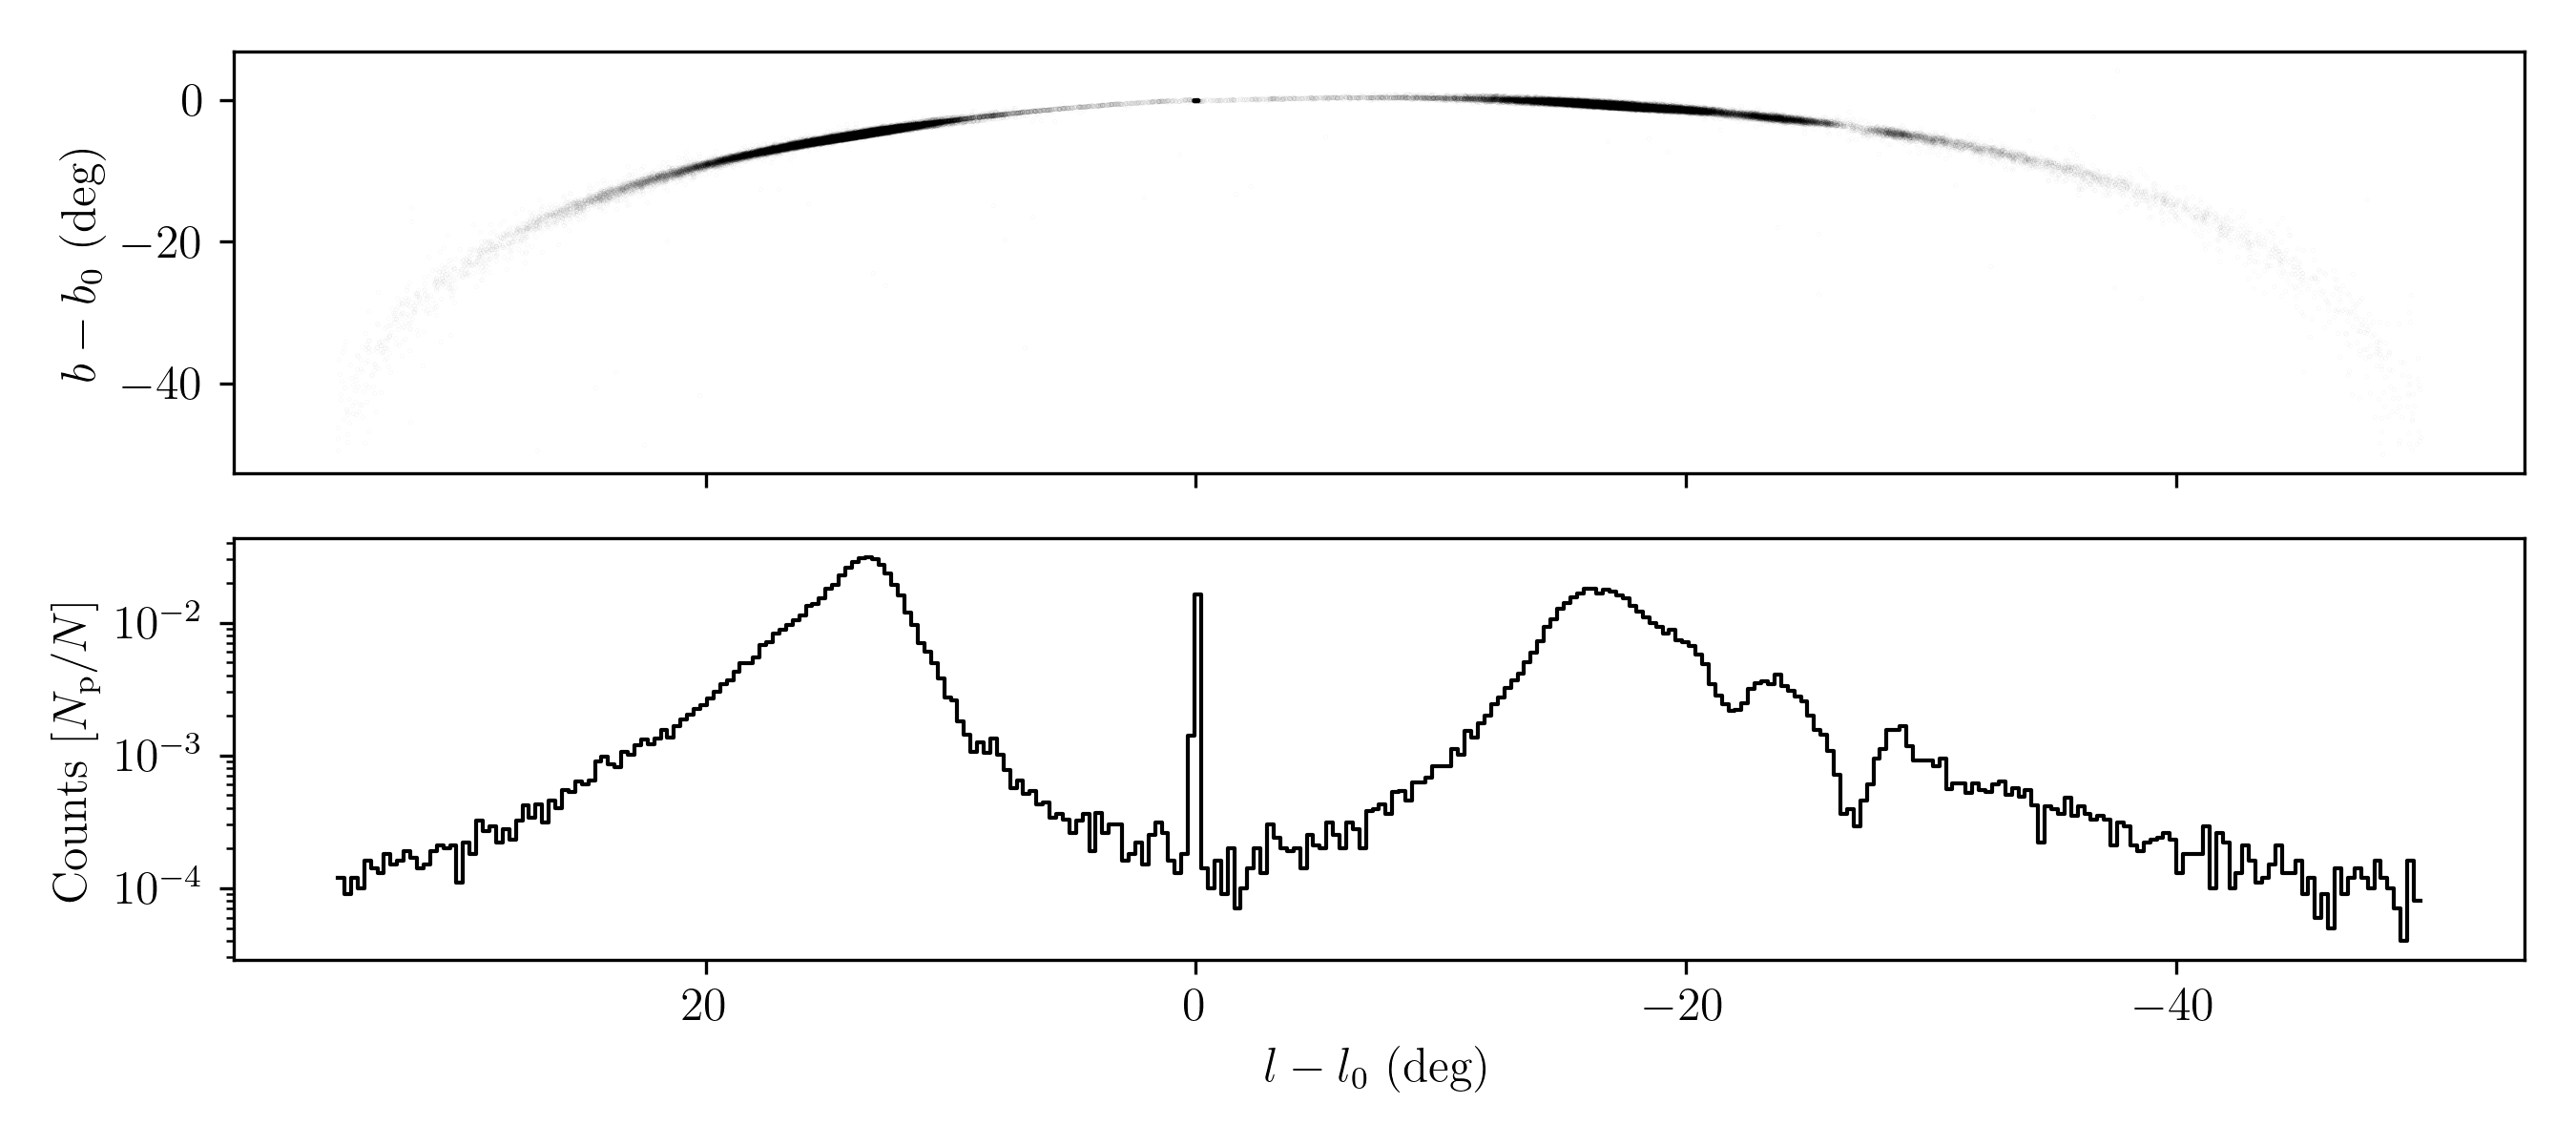
\includegraphics[width=\linewidth]{stream_on_sky_Pal5_monte-carlo-009_pouliasis2017pii-GCNBody.png}
    \caption{An instsance of the Palomar 5 stream created modeling the cluster as a plummer sphere within an axis-symmetric galactic potential plus 164 other galactic globular clusters. The top plot is a scatter plot of star-particles that escaped the cluster due to tidal forces, the bottom plot shows the marginalized 1D density profile in longitude. Two large gaps are present and are due to the passage of two globular clusters.}
    \label{fig:stream_on_sky}
    \end{figure*}










\section{Methods}



  \subsection{Numerical Methodology}
    Our numerical methodology follows the approach outlined in Ferrone et al. (2023), which we present here for completeness. We begin by extracting the phase space properties (positions, velocities) as well as the masses and half-mass radii of 165 globular clusters from the galactic globular cluster catalog by Baumgardt and Vasiliev et al. We handle the uncertainties through a monte-carlo approach. The catalog provides uncertainties for mass, distances, line of sight velocities, proper motions, with a covariance term between the proper motions. We repeate the whole experiment 50 times, for each of which we vary the initial conditions of each cluster by sampling its five-dimensional gaussian uncertaintiy distribution. However, for the first simulation, which we name \texttt{Sampling 000}, we use the most probable values for the initial conditions. 

    We convert the initial conditions from sky coordinates into a galactocentric reference frame. We use the local standard of rest and the peculiary motion of the sun as reported by Sch\"onrich 2010. The circular velocity at the solar radius was set to: $v_{\text{LSR}} = 240$~km~s$^{-1}$. The peculiar velocity of the sun was set to $(U_\odot, V_\odot, W_\odot)=(11.1, 12.24, 7.25)$~km~s$^{-1}$. The position of the Sun was set to $(x_\odot,y_\odot,z_\odot) = (-8.34,0,0.027)$~kpc, vertical position above the disk was taken from Chen et al 2001 and the galacto-radial distance was taken from Reid et al 2014. These transformations were performed using the \texttt{astropy} package. (for the next paper, I would also like to sample these uncertainties)

    For the galactic potential, we employed the second static model proposed by Pouliasis et al. (2017), which consists of a superposition of a thin disk, thick disk, and a dark matter halo. The masses and scale lengths are provided in Table 1 of Ferrone et al 2023. This model is time-independent over the course of our simulations. 

    The primary methodological departure from Ferrone et al. (2023) is that now we include globular cluster interactions. Instead of treating the clusters as point masses that only experience the gravitational potential of the galaxy, we now compute N-body interactions between the clusters during the backward integration over 5 billion years. The equation of motion for the globular clusters is thus: 
    \begin{equation}
      \ddot{\vec{r}}_i = -\nabla \Phi(R_i,z_i) + \left.\sum_{j\neq i} \frac{Gm_j}{\left(|\vec{r}_j - \vec{r}_i|^2 + b_j^2\right)^{3/2}}\right. \left(\vec{r}_j - \vec{r}_i\right).
      \end{equation}\label{eq:GCNBody}
    Although these interactions were included, we observed no significant exchanges of orbital energy or momentum between clusters. 

    At the computed positions 5 Gyr ago, each globular cluster was gifted a system of 100,000 particles, sampled from a Plummer distribution to represent the stellar content of the cluster. For eaching sampling of the initial conditions, a different sampling of the positions of the 100,000 star particles was performed. This is becuase, we sampled the uncertainties on the mass in this experiment contraty to Ferrone et al 2023. 
    
    We then integrated the evolution of these particles forward in time to the present day. During this forward integration, each star particle feels the gravitational influence of the galaxy and all globular clusters, but not other star particles. We do not perform direct N-body simulations between star particles as in eq.~\ref{eq:GCNBody}; instead, at each time step, we load the positions of all globular clusters, as found from the initial integration, and apply their forces to the star particles. The equation of motion is thus: 
    \begin{equation}
      \ddot{\vec{r}}_p = -\nabla \Phi(R_p,z_p) + \left.\sum_{j} \frac{Gm_j}{\left(|\vec{r}_j(t) - \vec{r}_p|^2 + b_j^2\right)^{3/2}}\right. \left(\vec{r}_j(t)- \vec{r}_p\right).
      \end{equation} \label{eq:equation_of_motion_particle}

    The integration was performed using a leapfrog integrator. The timestep was chosen to be sufficiently small to ensure both the conservation of energy and that the integration error over 5 Gyr was negligible compared to the scale radius of the globular clusters. Further details on the timestep selection are discussed in the appendix.

    During the integration, intermediate snapshots were saved to facilitate the analysis of stellar streams and the effects of cluster impacts. Specifically, for each of the 50 realizations of the Palomar 5 stream, we saved $5000$ intermediate timesteps which is a temporal resolution of 1 million years. To provide an estimate of the size of our simulations, we have $N_p=100 000$, $N_\textrm{time stamps} = 5 000$, $N_\textrm{phase}=6$, $N_\textrm{sampling}=50$, and using single precision floating point numbers, $\textrm{Single}=4$~bytes, results in approximately 600 GB of data.




  \subsection{Gap detection} \label{sec:gap_detection}

    At the end of the simulations, some gaps in the stellar stream are so prominent that they can be identified visually without any sophisticated quantitative analysis. However, upon closer inspection, more subtle gaps emerge, highlighting the need for quantitative methods to systematically detect and assess these features.

    We initially sought an automated, quantitative approach from signal and image processing that could reliably detect all gaps and evaluate their significance. Unfortunately, despite extensive efforts, an ideal method remained elusive. As a result, we opted for a simpler approach: a combination of visual inspection aided by comparative analysis.

    To facilitate this process, we ran a series of \texttt{vanilla} simulations. In these control simulations, we used the same 50 sets of initial conditions but excluded interactions between globular clusters and omitted the gravitational influence of the clusters on the star particles within the stream. By comparing the morphological differences between these control simulations and the full simulations (which included cluster interactions), we could identify and assess the impact of globular clusters on the stream structure more effectively.


    Comparisons between the \texttt{vanilla} and full simulations were performed in the tail coordinate system. This system allows for consistent morphological comparisons by aligning the stream with the cluster's orbit. The coordinate system is based on the work of Dehnen et al. (2004) and is detailed in Appendix~\ref{appendix:TailCoordinates}.

    Briefly, the x' coordinate represents the position of a particle along the orbit relative to the globular cluster—whether it is ahead or behind the cluster. The y' coordinate measures the particle's distance within the orbital plane, where positive values indicate that the particle is farther from the Galactic center and negative values indicate that it is closer.

    \subsubsection*{Density Maps and Profiles}
      For each of the 50 simulations, we compare the final snapshots between the \texttt{vanilla} and \texttt{full} simulations using the tail coordinate system. We inspect these differences by generating 2D density maps of the streams. Additionally, we marginalize over the $y'$-coordinate to produce 1D density profiles along the $x'$-axis. These comparisons are shown in the results section (see Fig.~\ref{fig:profiles}).

      \begin{figure*}
        \centering
        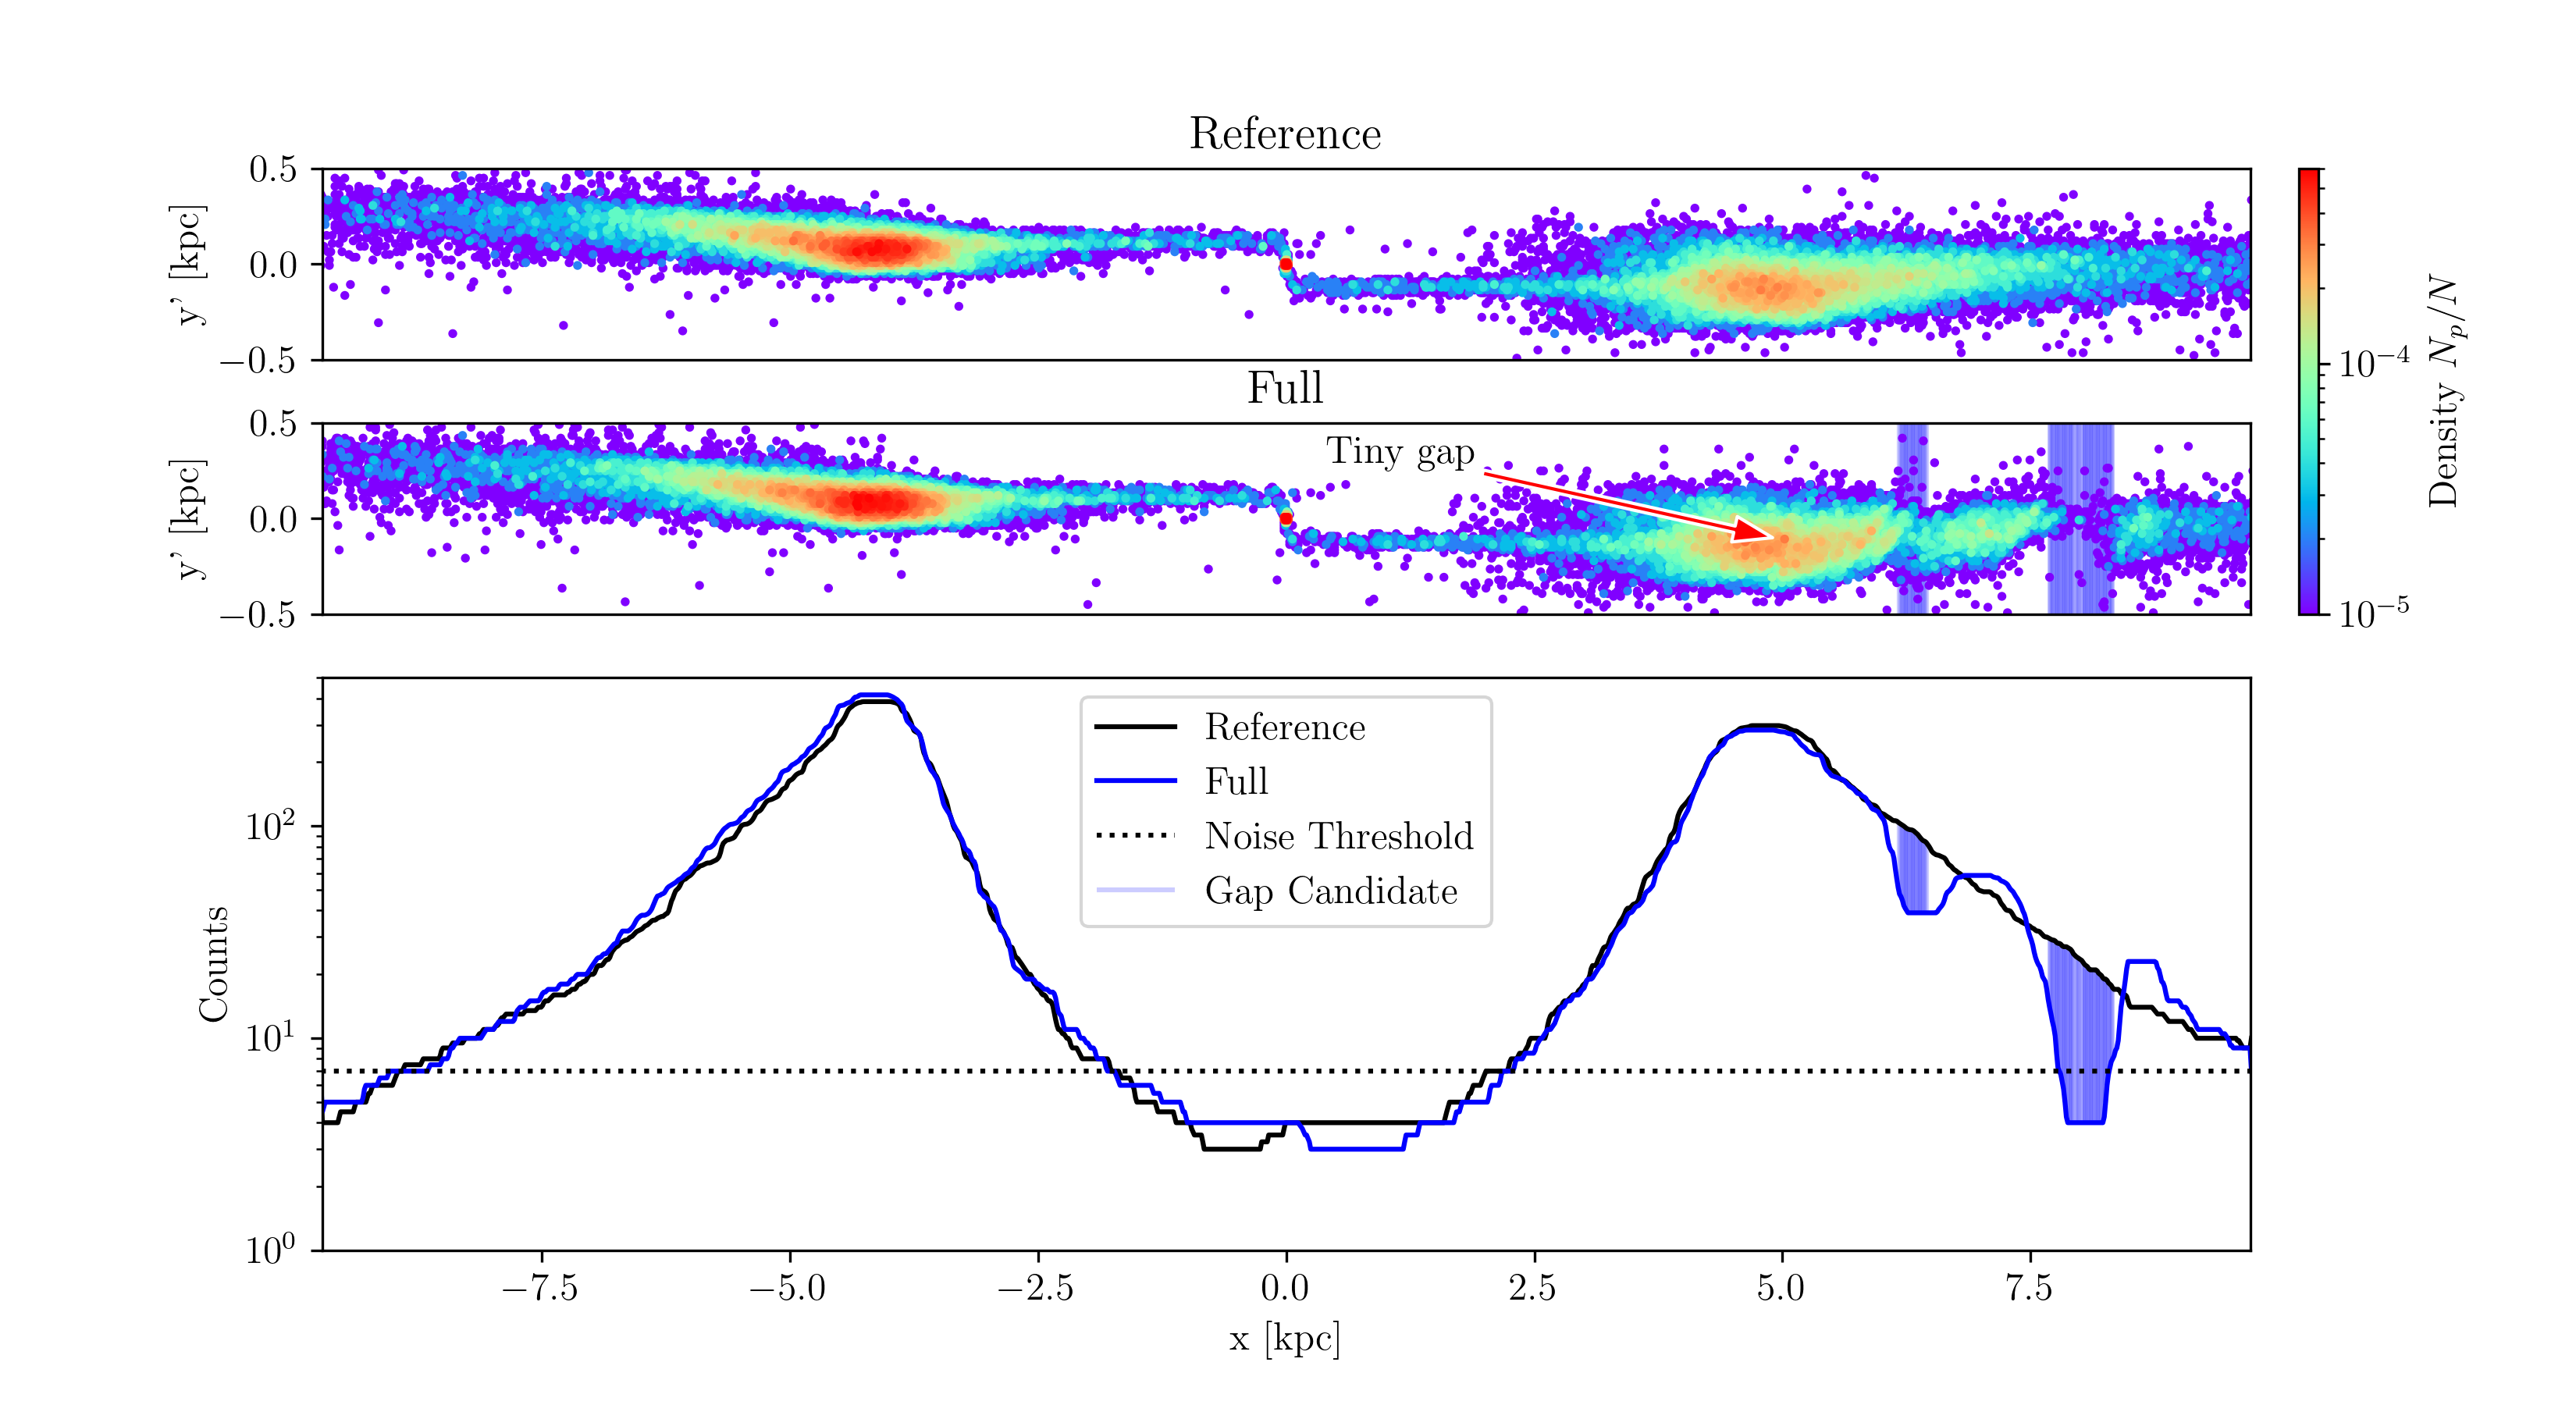
\includegraphics[width=\linewidth, trim=20 0 15 0]{monte-carlo-009-pouliasis2017pii-GCNBody-2000-milisigma-5-noisefactor-20-boxcarindexlength-shifted-0.png}
        \caption{A comparison between the density maps and profiles of the \texttt{full} and \texttt{vanilla} simulations is presented. The locations where the full simulation is less dense than the vanilla simulation by 2-$\sigma$ is highlighted by blue vertical bars. Bins below the noise threshold are not considered when measuring the differences between the two 1D profiles. The 1D profiles have been smoothed with a median box-car filter.}
        \label{fig:profiles}
        \end{figure*}

      To construct the 1D density profiles, we first bin the data using the $\sqrt{N}$ rule, where $N$ is the number of data points ($N_p = 10^5$). After binning the 1D profiles, we apply a boxcar smoothing technique. The density profiles are scanned. At each bin, a selected number of adjacent data points from both sides are placed in a list. The bin is then replaced with the median. We choose to use 10 adjacent points per side, which corresponding to a smoothing length of approximately 1~kpc. This procedure reduces high-frequency noise and smooths the profiles. For instance, notice the absence of a high mass peak indicating for the center of mass in the bottom panel of Fig.~\ref{fig:profiles}.

      With the smoothed 1D density profiles in hand, we treat the \texttt{vanilla} simulations as the reference model and search for regions in the \texttt{full} simulations that are significantly underdense compared to \texttt{vanilla}, surpassing stochastic fluctuations. To accomplish this, we first impose a signal-to-noise ratio threshold, $\mathcal{SNR}$. The signal is defined as the log of the counts per bin from the \texttt{vanilla} 1D density profile, and errors are propagated assuming a Poisson distribution. We then compute a threshold for the number of counts in the \texttt{vanilla} simulation, $N_v$, using the transcendental equation:
      \begin{equation}
          \mathcal{SNR} = \ln(10) \log_{10}\left(N_v\right) \sqrt{N_v}.
        \end{equation} \label{eq:density_threshold}
      By setting $\mathcal{SNR} = 5$, we solve for $N$ using \texttt{scipy.optimize.fsolve}, finding that $N$ must be greater than 7. After discarding insignificant bins (i.e., those with counts below the threshold), we compute the log ratio of the counts between the \texttt{vanilla} and full simulations:
      \begin{equation}
          \mathcal{R}_i = \log_{10}\left(\frac{N_{f,i}}{N_{v,i}}\right),
        \end{equation}
      where $\mathcal{R}_i$ is the log ratio, $N_{f,i}$ are the counts from the full simulation, and $N_{v,i}$ are the counts from the \texttt{vanilla} simulation for each bin $i$. We then analyze the distribution of $\mathcal{R}_i$. If the differences between the density profiles are primarily due to stochastic processes of similar magnitude, this distribution should resemble a Gaussian as expected from the central limit theorem. Thus, we flag all regions where the density is underdense by more than two standard deviations, which should highlight regions whose underdensity is unlikely to be the result of the sum of stochastic processess but rather the passage of another globular cluster. 

      This method, however, has its limitations, especially when detecting smaller gaps. As outlined by Erkal et al. (2015), a small gap is indicative of a weak impact, but rather a more recent one. This is because gap growth is a dispersion phenomenon. Additionally, since our streams have finite width, some gaps are oblique with respect to the stream axis. In such cases, marginalizing over $y'$ erases the gap's signal, making it impossible to detect in a 1D profile. This limitation is particularly evident in gaps caused by NGC~2808, as discussed in the results. Therefore, this quantitative analysis serves as an \textit{aid} to visual inspection rather than a complete substitute for it. This method helps particularly with large subtle gaps that the eye does not notice in the 2D maps.

    
    \subsubsection*{From Suspect to Culprit} \label{SuspectToCulprit}

      A key question we seek to answer is: from the gaps present at the end of the simulation, who caused them? To address this, we examine the evolution of stream density over time. Instead of using the x'-coordinate, we introduce $\tau$, which represents time rather than distance. Specifically, $\tau$ indicates how long it will take for a cluster to reach, or how long ago it passed, a given point on its orbit. This is advantageous because the growth of the stream is approximately linear in $\tau$ whereas in physical space, streams on eccentric orbits expand and contract depending on the orbital phase.


      \citet{sanders2016dynamics} extended the analysis of Erkal et al. (2015), demonstrating that action-angle variables provide a useful coordinate system for analyzing stream evolution, as actions are conserved and the angles associated with the stream's growth evolve linearly over time. Although we became aware of this work only after completing our analysis, we note that $\tau$ is a suitable approximation and behaves similarly to the angle variable corresponding to the azimuthal action: $\tau \approx \theta_{\phi,i} - \theta_{\phi,\text{GC}}$.

      The core of our analysis is presented in Fig.~\ref{fig:force-on-orbit}. The bottom panel shows the evolution of the stream density over time. To avoid extreme low-density regions at the stream's edges, we applied the same density threshold as from eq.~\ref{eq:density_threshold} to focus on the more significant areas of the stream. Next, we modeled Palomar 5's orbit as a proxy for its stream and sampled points along the orbit to measure the gravitational force exerted by other globular clusters. This force data is displayed in the top panel of Fig.~\ref{fig:force-on-orbit}, showing how the total gravitational acceleration on Palomar 5's stream evolves over its length throughout the simulation.

      \begin{figure*}
        \centering
        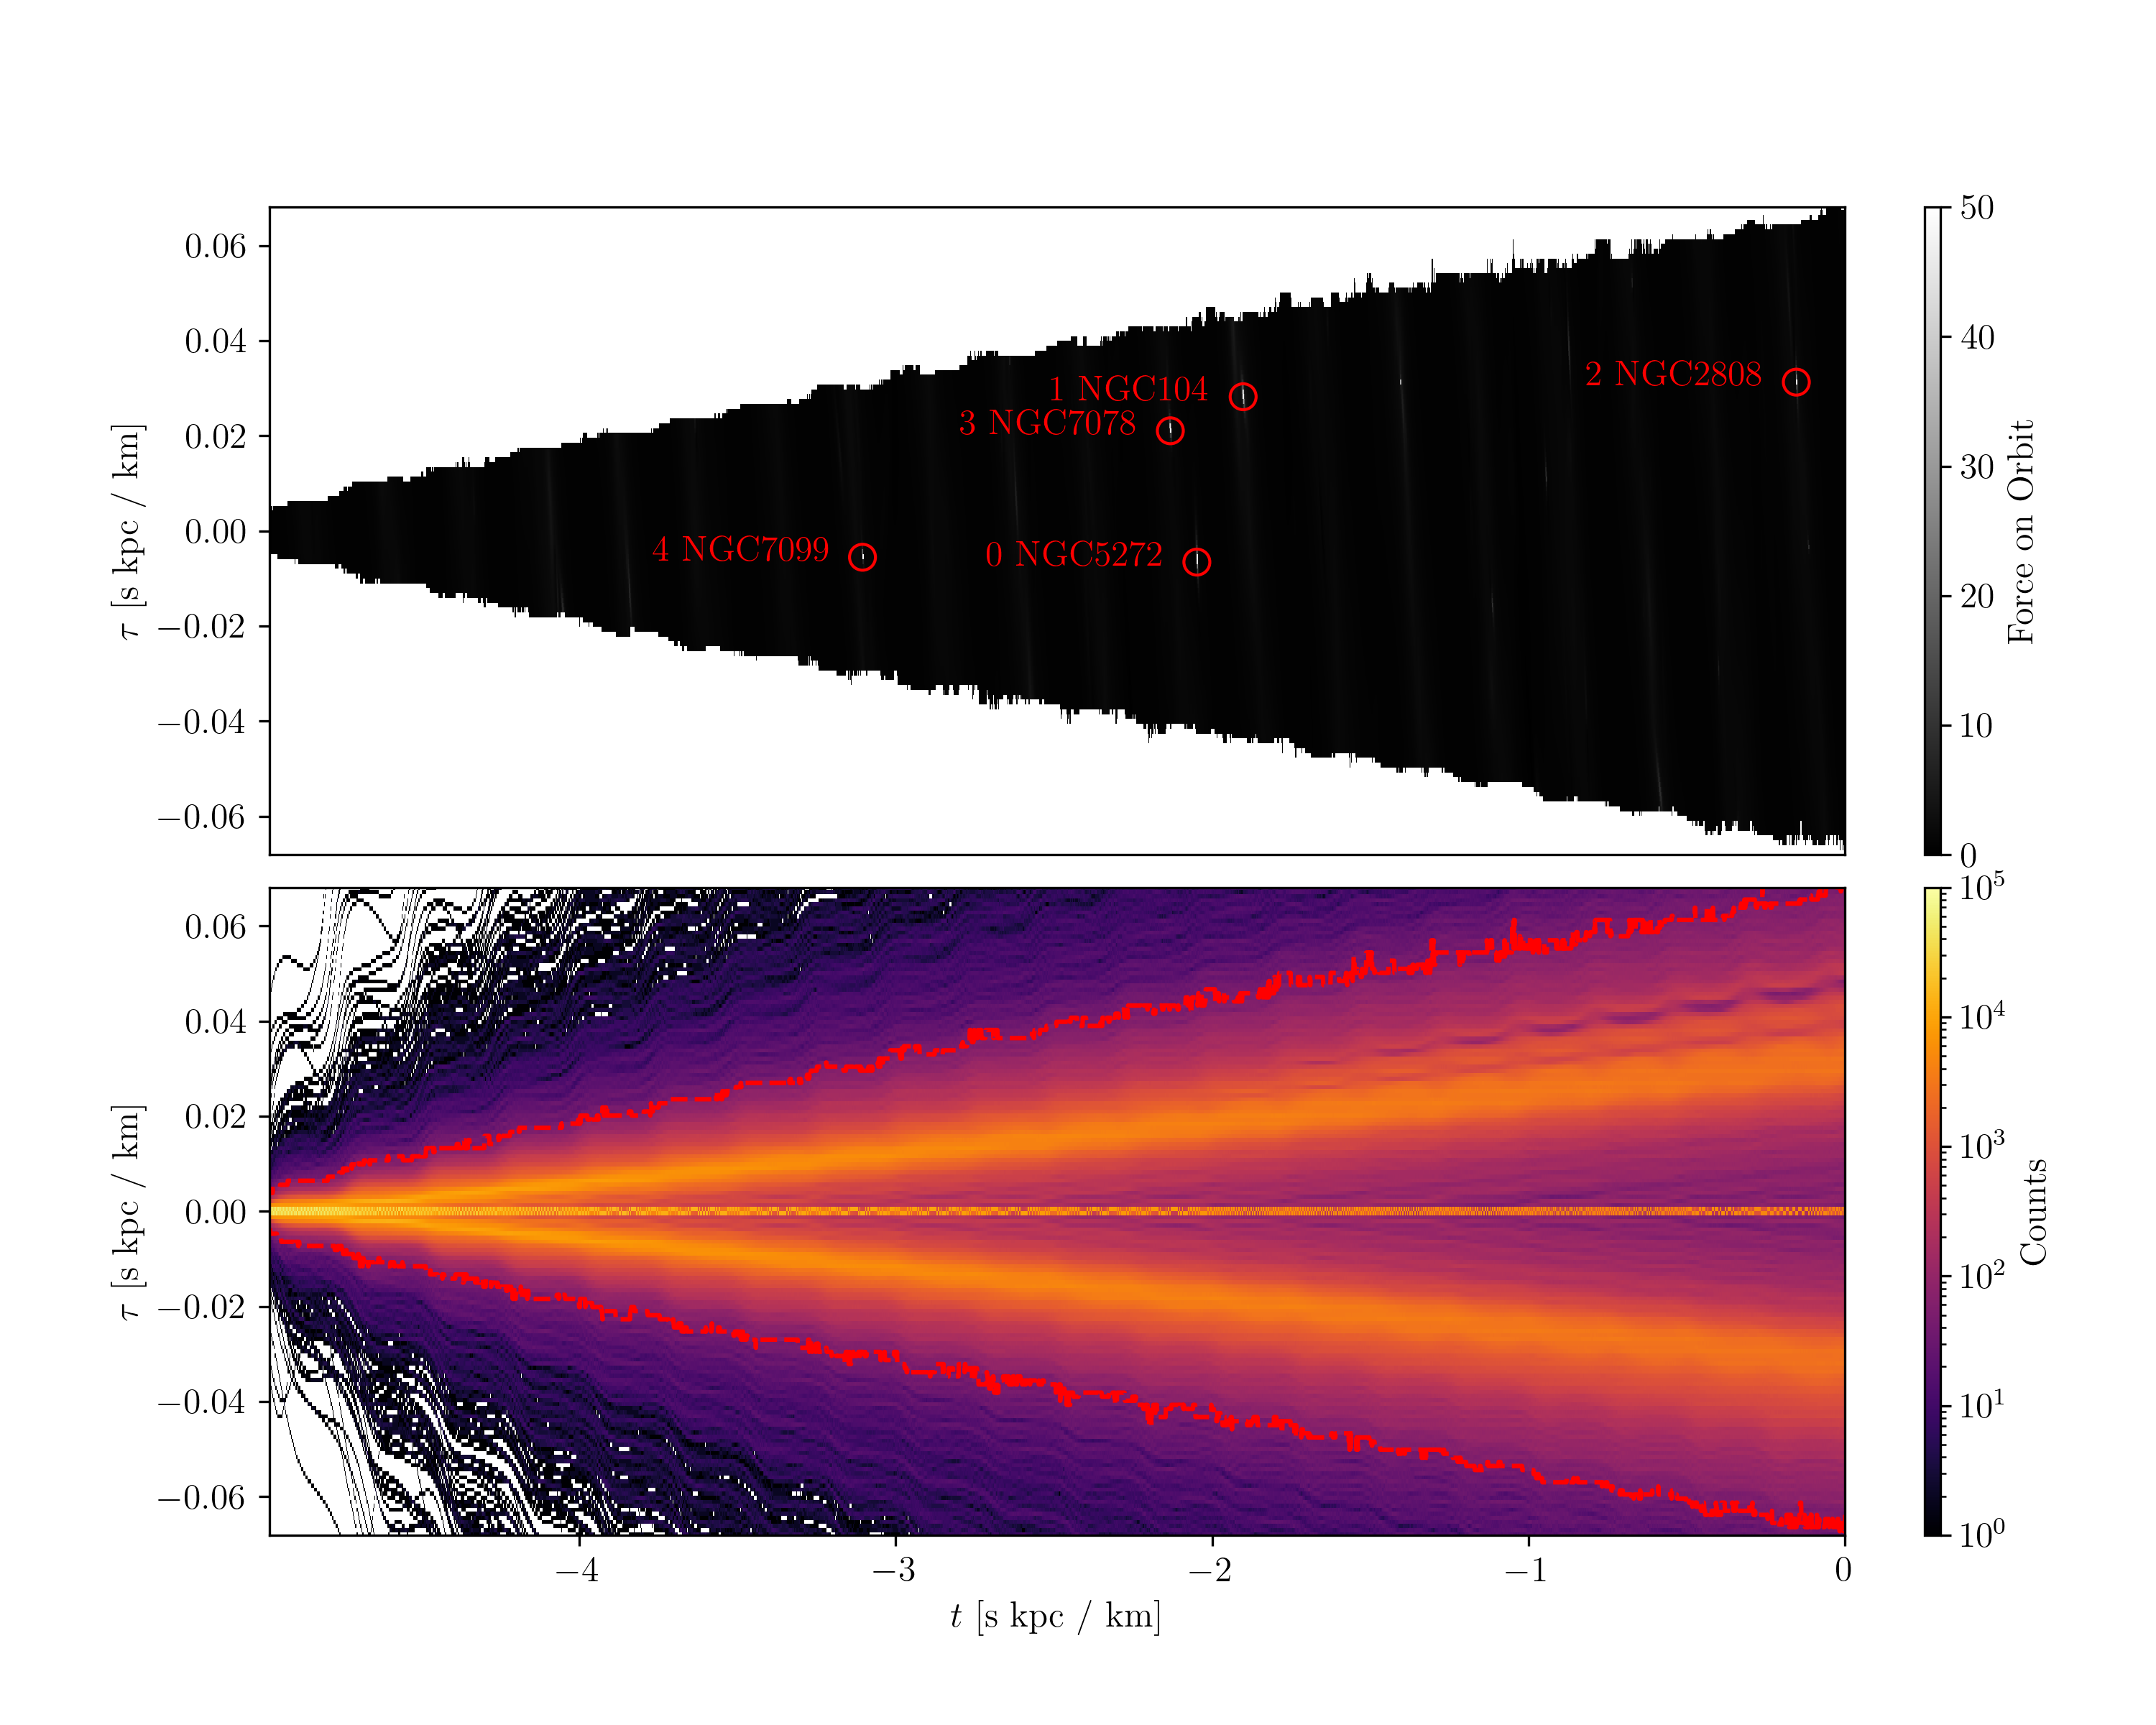
\includegraphics[width=\linewidth]{force_on_orbit-monte-carlo-009.png}
        \caption{This figure demonstrates how we determined which globular clusters were responsible for the gaps. The y-axis is $\tau$, which is a coordinate in units of time that indicates how far ahead or behind it is from a globular cluster. The x-axis is the simulation time, $t$, where 0~s km~kpc$^{-1}$ indicates present time.  The bottom plot showcases the evolution of the stream density in simulation time. The density was used to determine a sutible length of the stream as a function of time. This length was then used to extract a piece of Palomar 5's orbit about a given position of Pal 5 in time. This orbital segment is used to approximate the stream. Then, the gravitational force from all other clusers was computed on the orbit. This is shown in the top plot, where the gravitational force is in measured in acceleration and is given in integration units: km$^2$~kpc$^{-1}$~s$^{-2}$. Moments of high acceleration indicate the passage of another cluster. The top 5 strongest passages are labeled with red circles as well as the name of the clusters. The example shown in this plot is the same simulation as Fig.~\ref{fig:stream_on_sky}.}
        \label{fig:force-on-orbit}
        \end{figure*}  
    

      We then used \texttt{scipy}'s \texttt{ndimage} package to identify the top five local maxima in the data space of gravitational acceleration $\vec{g}$ as a function of time $t$ and the stream coordinate $\tau$. TheThis is done by first smoothing the image by taking a 5 point moving average kernel. Secondly, we use maximum filter to locate coordinates in the $t,\tau$ data plane who are local maxima to at least 10-adjacent data points. These locations are then ordered and the top five strongest interactions are saved. Once these local maxima were identified, we iterated over the contributions of individual globular clusters to determine which cluster contributed the most to each peak in $\vec{g}$. Each significant peak was labeled with the corresponding globular cluster.


      Afterward, we cross-referenced these peaks with the locations of the gaps identified by studying the density maps and profiles from Fig.~\ref{fig:profiles}. For large gaps resulting from strong interactions, we observed that after an impact, a low-density wake is left behind in the ($t,\tau$) plane, which can be seen corresponding to the impacts of NGC~104 and NGC~7808 in the bottom panel of Fig.~\ref{fig:force-on-orbit}.

      The results of this analysis were compiled into a table. If a gap was attributed to a particular globular cluster, it was labeled as \texttt{TRUE}; otherwise, it was marked as \texttt{FALSE}. For a handful of simulations, to double check that the verdict made correctly when passing from suspect to culprit, we re-compute the simulations yet individually adding one globular cluster at a time. As a result, we are able to confirm that singular gaps arrise from the suspected clusters, an example of which is shown in Fig.~\ref{fig:decomposition}. 

      \begin{figure*}
        \centering
        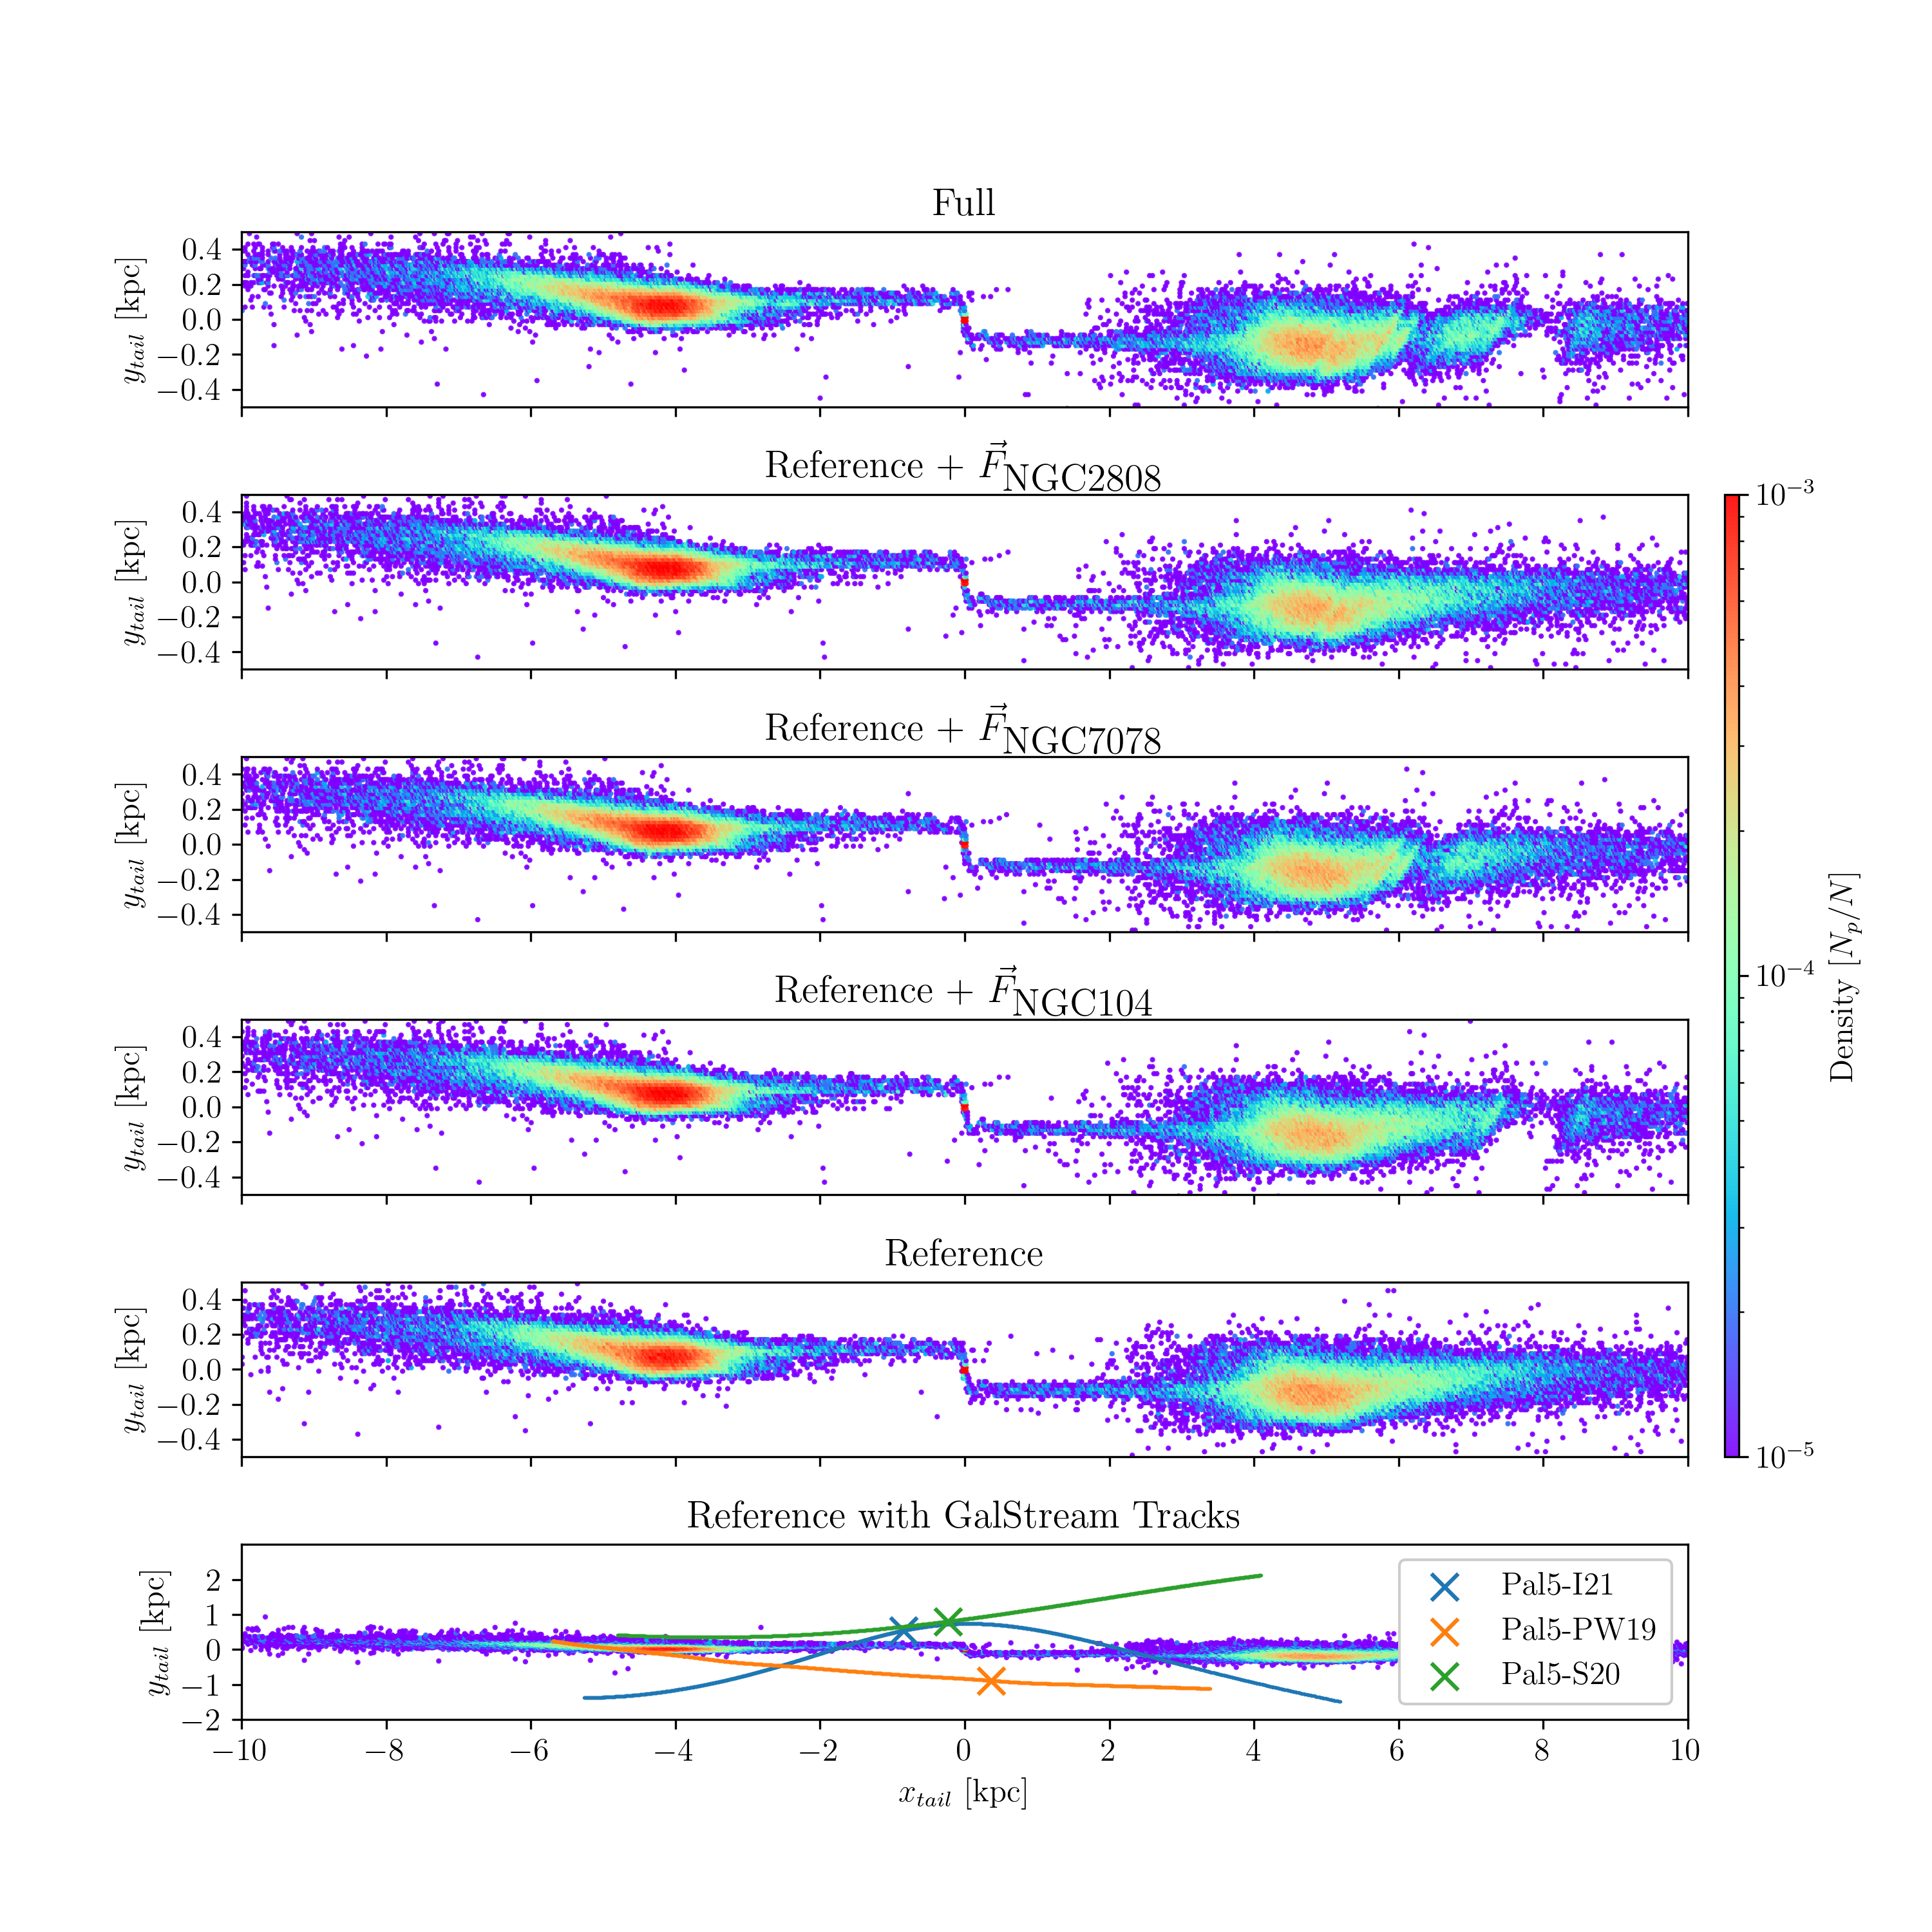
\includegraphics[width=\linewidth]{decomposition-monte-carlo-009-with-3-gaps.png}
        \caption{This figure decomposes the gaps shown in the middle panel of Fig.~\ref{fig:profiles} into the individual perturbuers whose cause them, as identified from Fig.~\ref{fig:force-on-orbit}. These simulations only include the suspected globular clusters in one-at-a-time.}
        \label{fig:decomposition}
        \end{figure*} 

  \subsection{Reconstruction of the impact geometry}
    
    With the perturbers identified, we perform statistics in the pursuit of understanding what conditions are necessary for a globular cluster and a stream to have in order for a gap to form. We turn to impact theory, which in its simplest form as presented in works such as Binney and Tremaine, John Taylor, and Galaxiesbook, considers two particles: one stationary and the other moving past it. The distance between the two particles at their closest approach is known as the impact parameter. To simplify the analysis, the \textit{impulse approximation} is often employed, which assumes that the velocity of the perturber remains unchanged during the interaction. This assumption greatly simplifies the computation.

    To understand how the impacted particle is perturbed, one needs to compute its change in momentum, which is determined by integrating the force acting on the particle over the duration of the interaction. A useful approximation for this change in momentum is the force at the closest approach multiplied by an estimate of the interaction time:
    \begin{equation} 
      \Delta p \approx \text{Force} \times \text{interaction time} = \frac{GMm}{b^2} \times \frac{b}{v} = \frac{GM}{bv}, 
      \end{equation} \label{eq:change_in_momentum}
    where $M$ is the mass of the perturber, $m$ is the mass of the particle, $b$ is the impact parameter, $v$ is the relative velocity of the perturber with respect to the particle, and $G$ is the gravitational constant.

    From this analysis, we can conclude that a more massive perturber, passing closer to the particle, and moving more slowly, will have a greater impact. It's important to note that the momentum change is inversely proportional to the velocity of the perturber, which contrasts with the intuition from elastic collisions, such as those between billiard balls, where higher velocities result in greater impacts.

    Erkal et al. (2015) extended this impact theory from one point mass impacting another point mass, to studying how an extended body impacts as stream. This quantifies the change in momentum of a given particle as a function of its distance from the point of greatest impact. In their analysis, the perturber was modeled as a Plummer sphere. Since the stream is not zero-dimensional and has length, both the parallel and perpendicular components of the velocity must be considered. Consequently, five parameters determine the change in velocity of a given particle: $M$, $r_p$, $b$, $W_\parallel$, and $W_\perp$. Our goal is to constrain these parameters during the impact in our simulations and compare them to close approaches that do not generate gaps, in order to establish the criteria necessary for gap formation.

    To achieve this, we begin by identifying the approximate moments of impact from the most significant clusters, as determined in the previous analysis in Sec.~\ref{SuspectToCulprit}. Then, we refine these estimates. While the orbit serves as a good first-order proxy for the stream, it is insufficient, as the typical offset between the stream and its orbit can be on the order of 200-400 pc—--significantly larger than the impact parameters we are investigating.

    In this refinement process, we aim to pinpoint both the exact location of the impact along the stream and the precise moment it occurred. To do so, we fit a third-order parametric polynomial to the stream, using the saved snapshots from our simulations:
    \begin{equation}
      \vec{s}(\tau) = 
      \left\{
        \begin{aligned}
          x(\tau) &= a_0 + a_1 \tau + a_2 \tau^2 + a_3 \tau^3 \\ 
          y(\tau) &= b_0 + b_1 \tau + b_2 \tau^2 + b_3 \tau^3 \\
          z(\tau) &= c_0 + c_1 \tau + c_2 \tau^2 + c_3 \tau^3
        \end{aligned}
      \right.
      \end{equation}  
    where $x$, $y$, and $z$ represent the parametric line describing the stream in galactocentric coordinates, $\tau$ is the stream coordinate in time as described in the previous section, and is used as the independent variable to parameterize the motion. The coefficients $a_i$, $b_i$, and $c_i$ are the polynomial coefficients. We found that a second-order polynomial was insufficient to capture the curvature along the full length of the stream, with divergence from the star particle positions occurring at the extremes. A third-order polynomial was sufficient and desirable, as it is the lowest order that adequately captures the path of the stream over the entire length under consideration.

    In this analysis, only one side of the stream is considered. For instance, if the impact candidate was in the leading tail, only the star particles with $\tau > 0$ are used to constrain the stream track. The polynomial coefficients were determined using the through a minimization method using Nelder-Mead algorithm from \texttt{scipy}'s optimization package.

    Since the simulation snapshots were saved at a temporal resolution of 1 Myr--—rather than at the integration timestep, which would have generated an excessive amount of data—--we interpolate between snapshots to more precisely estimate the impact geometry. This is achieved by fitting the stream at five timesteps surrounding the approximate impact time, a period of 5 Myr, which sufficiently covers the interaction time. The interaction time can be estimated as $t \approx \frac{100~\text{pc}}{300~\frac{\text{km}}{\text{s}}} \approx 0.3~\text{Myr}$.

    As a result, each polynomial coefficient can now be expressed as a function of time. Consequently, we can parameterize the stream as a function of both simulation time and position along the stream:
    \begin{equation}
      \vec{s}(t,\tau) = 
      \left\{
      \begin{aligned}
        x(t,\tau) &= a_0(t) + a_1(t)\tau + a_2(t) \tau^2 + a_3(t)\tau^3 \\ 
        y(t,\tau) &= b_0(t) + b_1(t)\tau + b_2(t) \tau^2 + b_3(t)\tau^3 \\
        z(t,\tau) &= c_0(t) + c_1(t)\tau + c_2(t) \tau^2 + c_3(t)\tau^3.
        \end{aligned}
      \right.
    \end{equation}
    The values of the coefficients as a function of time are obtained through linear interpolation, ensuring that the coefficients at the snapshot times match the values constrained by the simulation data.

    Next, we fit the trajectory of the perturber with a second-order polynomial. With equations for both the stream and the perturber as functions of time, we identify the time and location of impact by minimizing a cost function, defined as the distance between the stream and the perturber:
    \begin{equation} 
      b(t, \tau) = \left\lVert \vec{s}(t, \tau) - \vec{p}(t) \right\rVert, 
      \end{equation}
    where $\vec{s}(t, \tau)$ is the galactocentric position of a point on the stream, $\vec{p}(t)$ is the position of the perturber, and $b$ is the distance between the two. The minimum value of $b$, denoted as $\text{min}(b)$, represents the impact parameter. The minimization is carried out using \texttt{scipy}'s optimization package with the \textit{L-BFGS-B} method, which allows us to constrain $t$ and $\tau$, ensuring no extrapolation occurs.

    Once this minimization is performed, determining the relative velocity becomes straightforward. Since the minimization provides the impact parameter, time of impact, and corresponding value of $\tau$, we can compute the derivatives of the parametric equations at $t_{\text{min}}$ and $\tau_{\text{min}}$. The parallel and perpendicular components of the perturber's velocity relative to the stream are given by:
    \begin{equation}
      \begin{aligned}
        \delta \vec{v} &=\vec{v_p} - \vec{v_s} \\
        w_\parallel &= \left(\delta \vec{v}\right)\cdot \hat{v_s}\\  
        w_\perp &=  \sqrt{\Delta v ^2 - w_\parallel ^ 2}
        \end{aligned}
      \end{equation}
    where $\vec{v}_p$ and $\vec{v}_s$ are the velocities of the perturber and the stream, respectively. For each of the 50 simulations, this information was compute for the strongs 5 flybys of a perturber with the stream. Thus, we compute a sample of 250 impacts, and flag those that give way to gaps. 


\section{Results}

  One of the 50 simulations is shown in Fig.~\ref{fig:stream_on_sky}--which we selected for its clear and prominent gaps which are visibile in the scatter plot of the stars on the sky and becomes even more apparent when marginalizing over latitutde to see it's 1D density over longitude. 

  We then transformed the stream to tail coordinates for the both the \texttt{vanilla} and \texttt{full} simulations in Fig.~\ref{fig:profiles}. As described in section~\ref{sec:gap_detection}, we locate regions on the stream where the full simulations are significantly less dense than the vanilla simulations. Notice the \textit{Tiny Gap} labeled in the middle plot. This signal is not present in the 1D profile since it is too small in size and at an oblique angle, thus is lost when marginalizing. This process was followed for all 50 simulations to identify possible gaps. We find that small gaps are identifiable by eye rather well, where the 1D profiles aid in finding subtle yet extended underdensities. All simulations and labeled gaps are presented in the Appendix~\ref{appendix:gallery_of_gaps}. The profile method was useful in identifying the subtle underdense gaps of Samplings: 000, 002, 006, 024, 028, 029, 030, 044, \& 048. 
  
  Besides gaps, a handful of simulations show the entire stream laterally shifted in tail coordinates. The most extreme case was observed in Sampling 006 and is presented in the Appendix~\ref{appendix:gallery_of_gaps}. This hampered our 1D profile difference analysis whose based the assumption that any difference in density would be due to the passage of other globular clusters and thus under densities. To combat this, we performed a cosmetique data reduction where I moved the \texttt{Full} 1D profile to best overlap with \texttt{Vanilla} by computing the correlation integral. Since this is not the focus of this study, we did not investigate further. We conjecture that the translation may arrise from a resonance phenomenon, most likely coming from Omega Centauri. Perhaps, in some orbital configurations Palomar 5 and Omega Centauri pass each other in regular intervals that can accelerate the globular cluster differently from the stream. 
  


  The clusters that impacted Palomar 5's stream in our simulations are presented in Fig.~\ref{fig:histogram_impact_time}, along with when they impacted the stream. First, there are few impacts that happen early on in the simulation. This is not surprising, as it the tidal tails are smaller and thus there is less volume to be perturbed. Next, is that 44/50 simulations contain a visible gap from NGC2808, all of the encounters occuring about 200~Myr ago. This is so much more than any other peak that we broke the scale of the histogram. The reason is that the uncertainty in the precise position of the clusters along their orbits grows in look back time. Since this encounter is recent, most of the sampled initial conditions give rise to a significant enough impact in the stream that causes a gap.

  \begin{figure*}
    \centering
    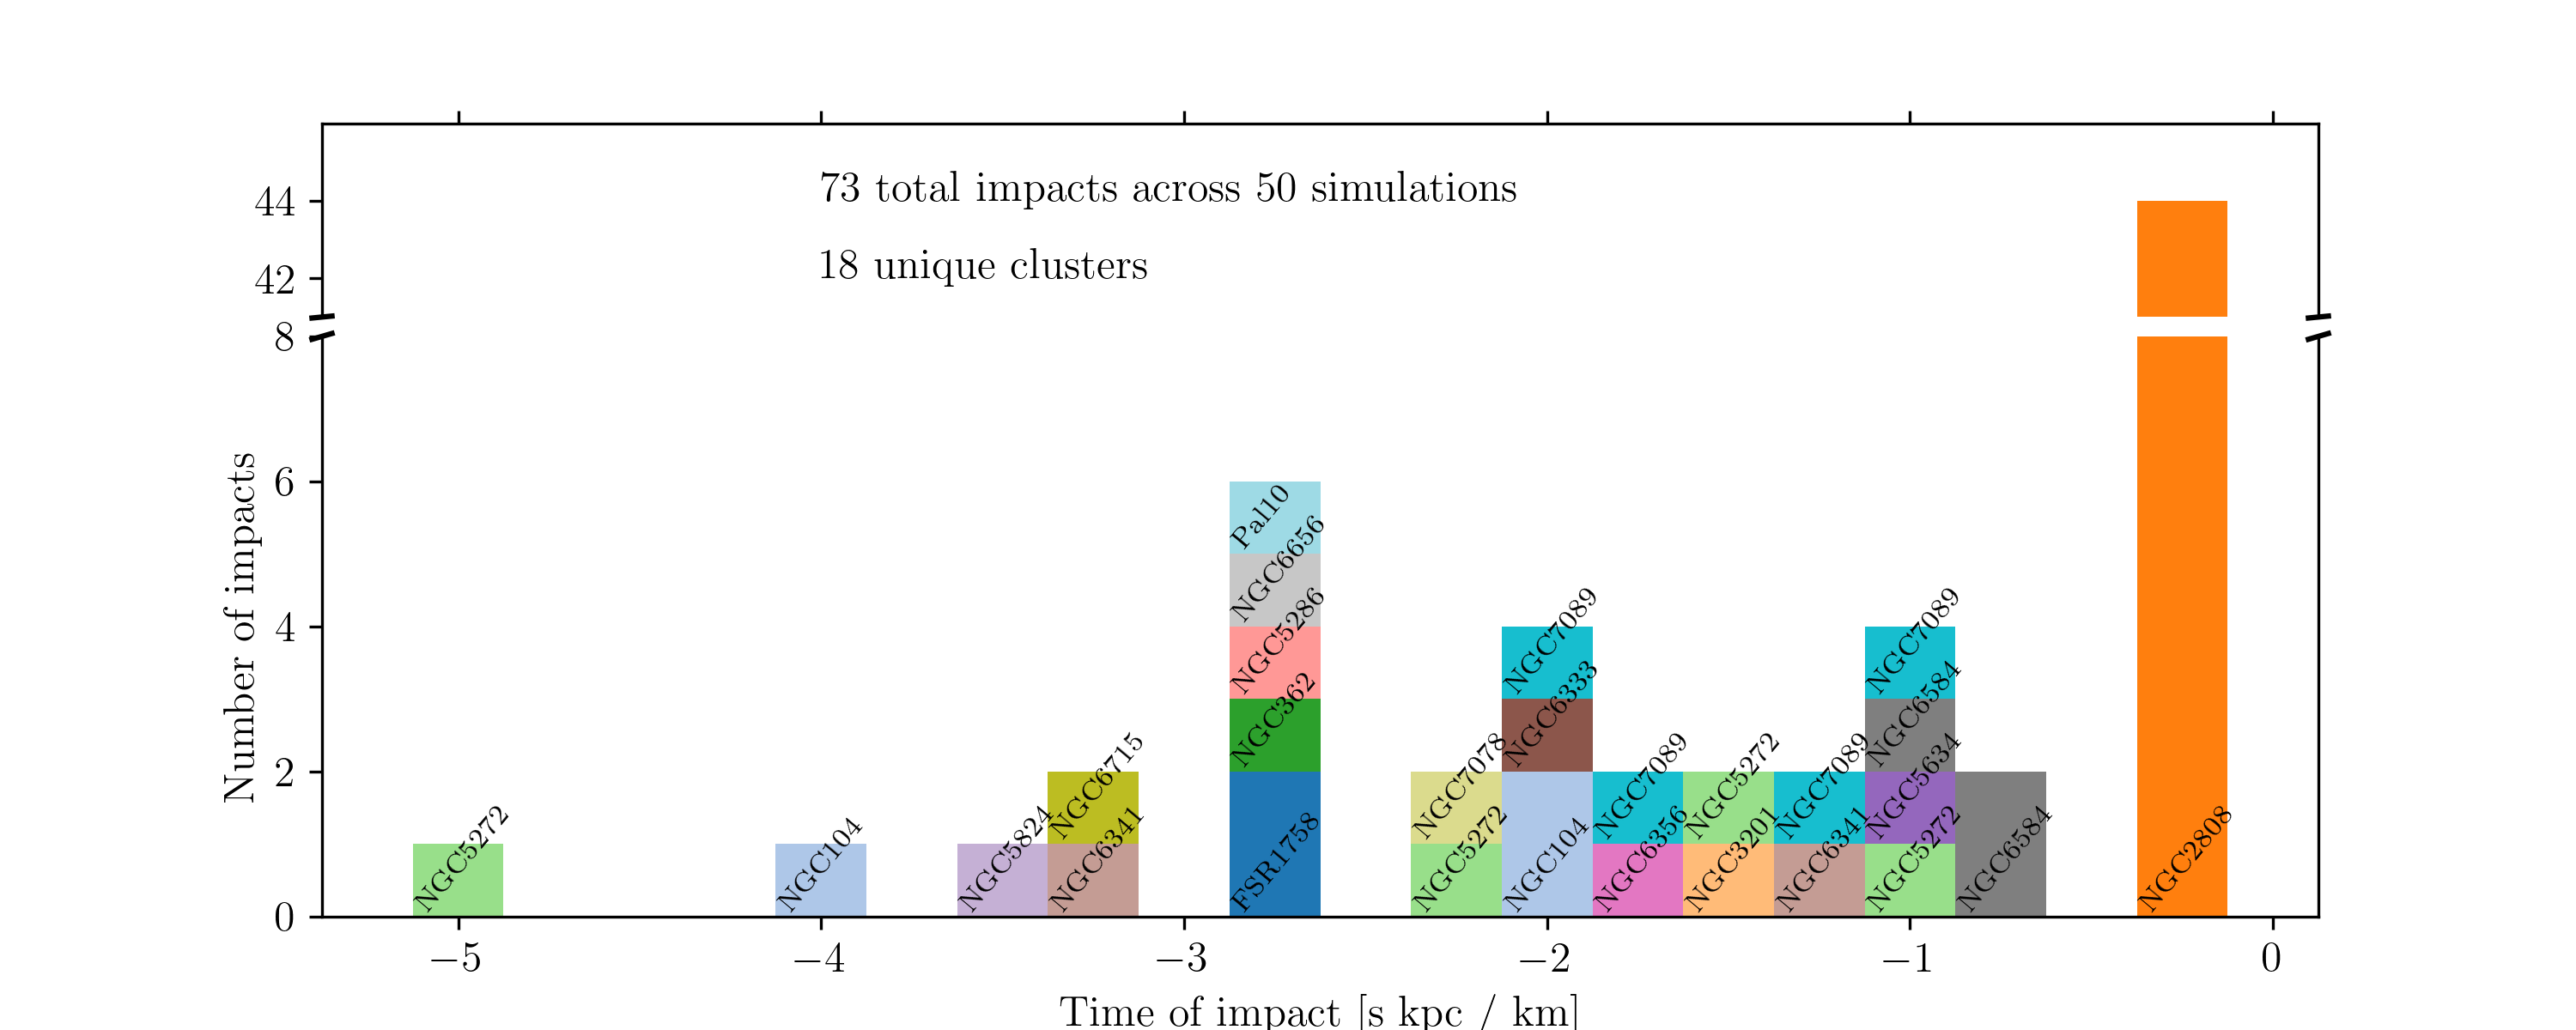
\includegraphics[width=\linewidth]{histogram_impact_time.png}
    \caption{When the impacts occured}
    \label{fig:histogram_impact_time}
    \end{figure*}  

  To speak on the morphological of gaps, the passage of globular clusters has not effected the width of the streams, i.e. they have not made them dynamically \textit{warmer}. The flybys gently impart a change in momentum on a local patch of particles and general pushes them to the side. As identified in Erkal et al 2015, the width of a gap is determined by how long ago the impact occured, while the depth of a gap is more indicative of how hard it was hit. 

  The quantities of the gap that perhap define how much of a gap it is, would be the width and the depth. We do not attempt to quantify this in this study. However, there are very few simulations that have both wide and deep gaps. These are the most prominent gaps and come from NGC104 and NGC7078 on Sampling 009, NGC104 on Sampling 027, NGC7089 on Samplings 035, 049. 



  We desire to search for some generalizable characterisitcs of the perturbers to see what contrasts them to globular clusters that do not impact the Pal5 Stream. We present three different graphs in Fig.~\ref{fig:mass_size_plane}. The top plot shows the angular momentm and energy plane. The 


    
    - to no surprise, you have to come within Palomar 5's orbital space 
    
    - trying to separate to the components of the velocity, Mass, impact parameter is not fruitful. It's better just to look at the change in momentum as given in the EQ.
    
    - Notice that the distributions between the gap and no gap are significantly different, yet also have significant overlap. Perhaps these 3 parameters don't tell the whole story but also there's the factor identifies in Sanders, that I don't understand yet, that shows that a gap will not be identifiable. 
  
  \begin{figure}
    \centering
    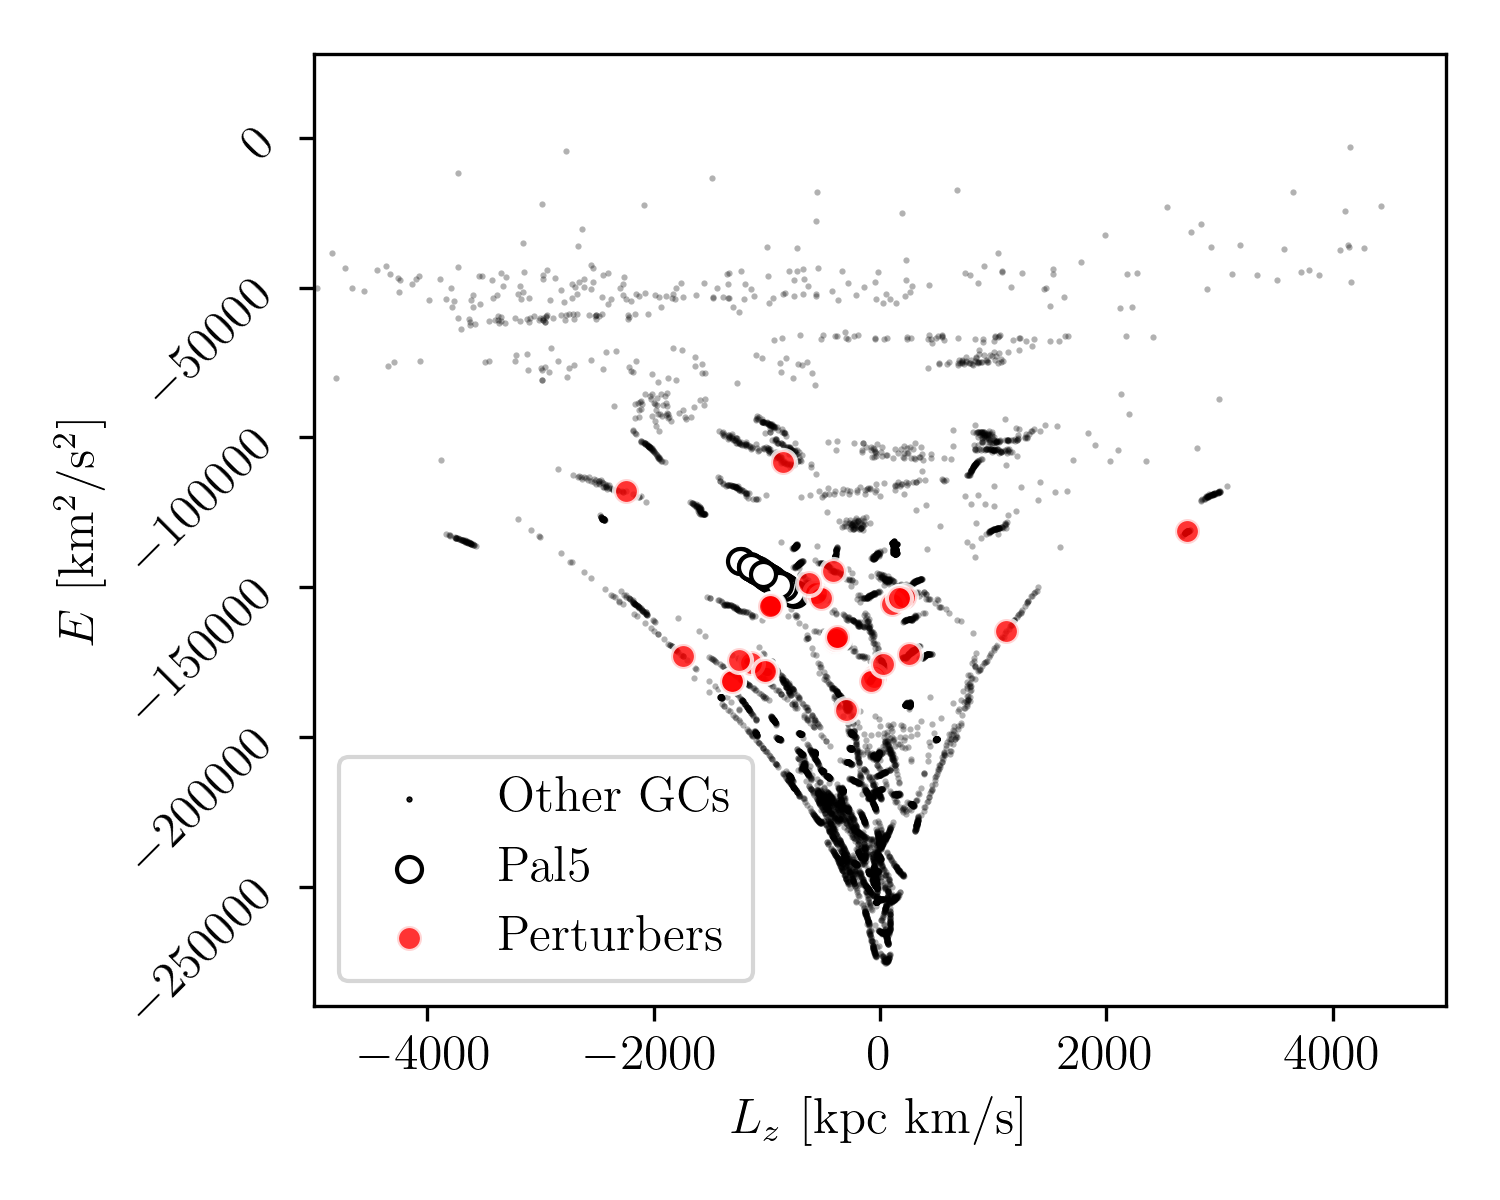
\includegraphics[width=1\linewidth]{E_Lz_perturbers.png}
    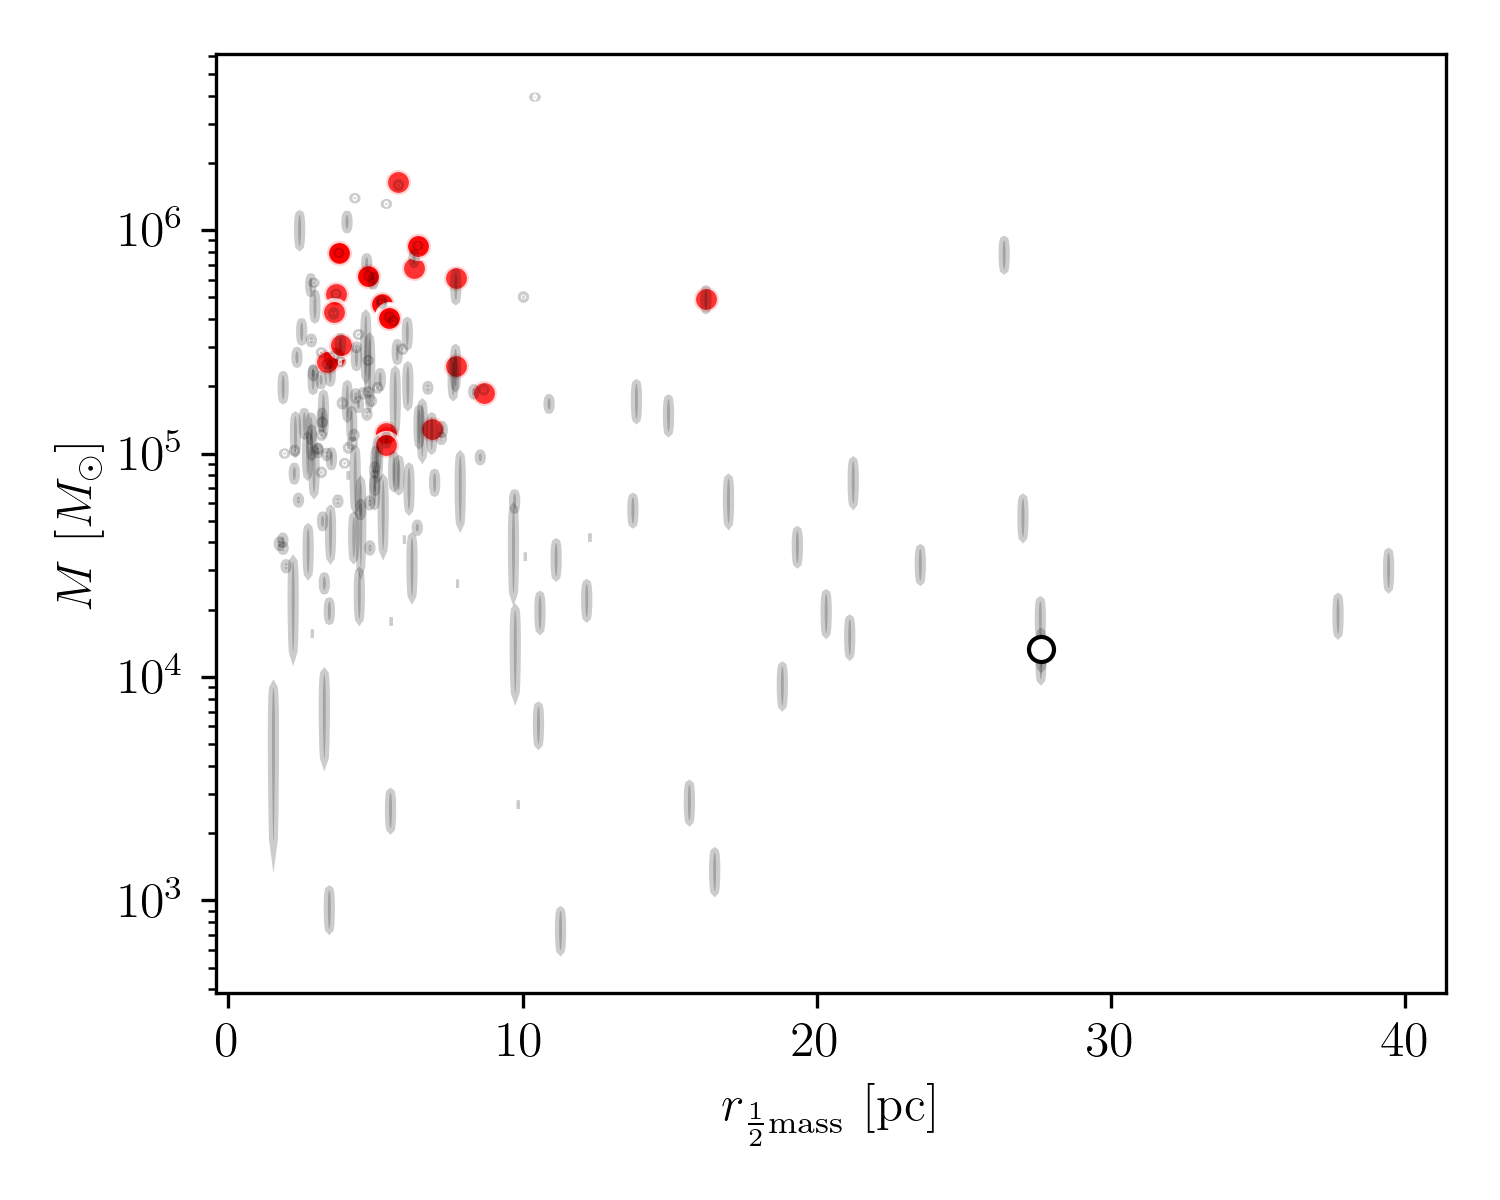
\includegraphics[width=1\linewidth]{mass_size_plane.png}
    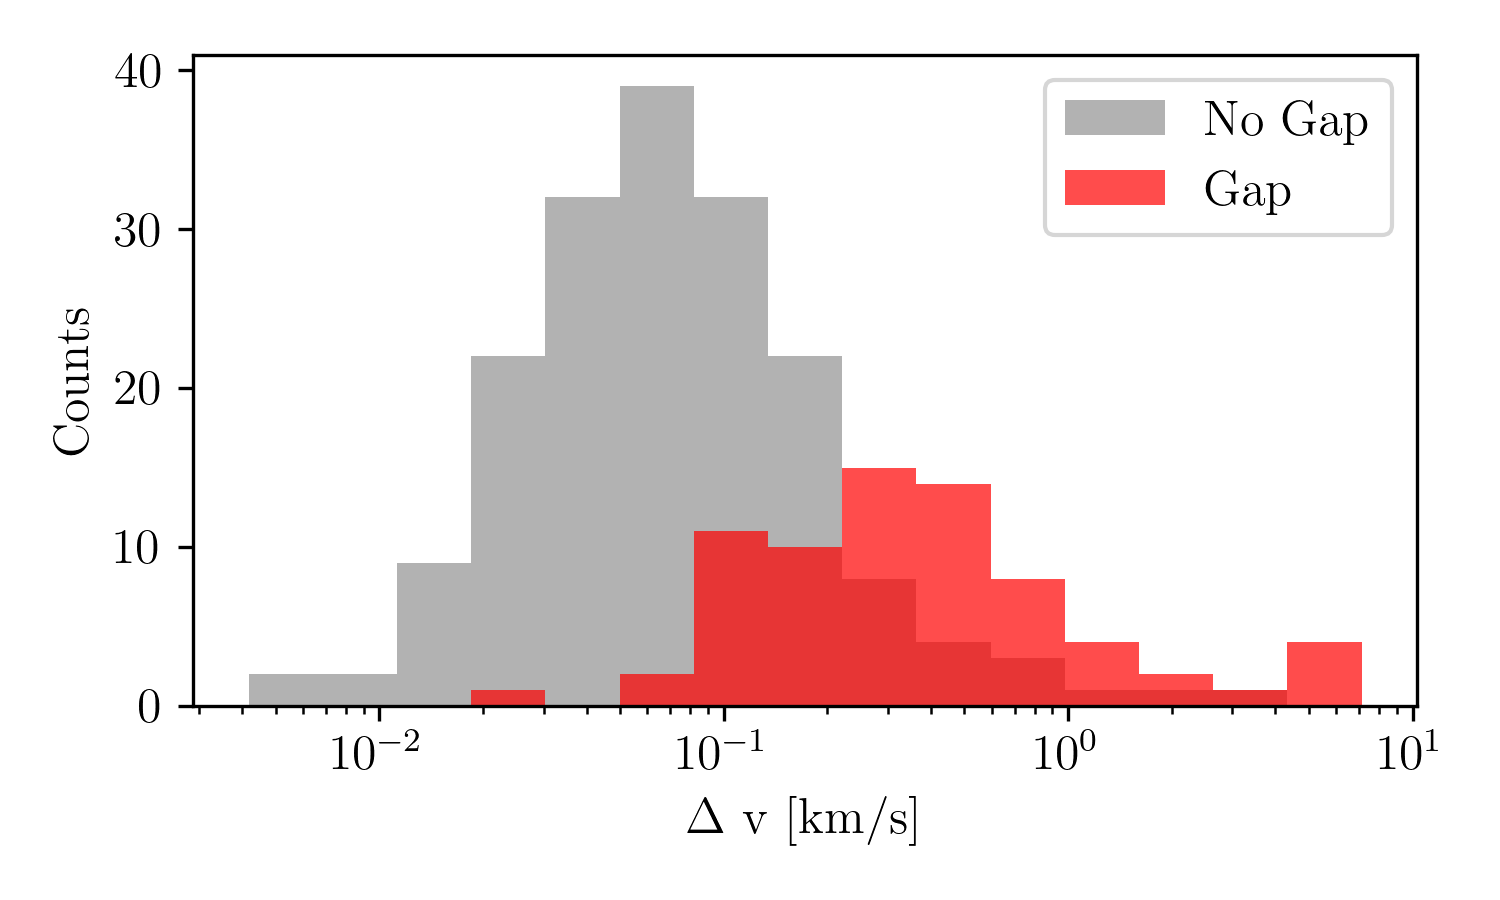
\includegraphics[width=1\linewidth]{impact_geometry_statistics_deltaP.png}
    \caption{Characterisitcs of clusters that cause gaps compared to those that do not. \textbf{Top:} shows the energy-angular momentum space of the globular clusters present in the simulations. Notice that we include all initial conditions that were sampled, therefore there are 50 $\times$ 165 data points. The clusters of a given simulation that impacted Palomar 5 are given with a Red marker, while non-gap causing clusters are given in gray. \textbf{Middle:} The mass-size plane. Uncertainties on the mass are indicated, while no uncertainties on the radius were reported. \textbf{Bottom:} the imparted momentum on the star-particles from a given flyby as given in Eq.~\ref{eq:change_in_momentum}. The top 5 strongest flybys from each simulation are included in this dataset, those that cause gaps are flagged.}
    \label{fig:mass_size_plane}
    \end{figure}


  
  
  After we discuss the magic to make detections, I THEN will discuss some general properties, i.e. is there something special about these perturbers compared to other clusters? The main results is that \textit{you need to enter Pal5's orbital space}, which is not a shocker. If you can hit me, you can't perturb me. NEXT, I want to compare the population of perturbers to all globular clusters based on their internal parameters, so here we do show a tendency. Next, I wanna show how often gaps appear, and thus how many time a given GC pertubered Pal5, and when the gaps occur. I think a conclusion with the histograms in time is 

  Lastly, I will try to show something about the impact geometry. I will state that we want to compare the ones that create gaps to those that did not. We wanted to apply what we learned from Carlberg, Erkal and Sanders. The moral of the story will be that, no combination of parameters explaining the geometry cleared demarcated the presence of a gap or not. This can be inline with Sander's expanion of the analysis initiated by Carlberg and extended by Erkal. Namly, a uniformly dense stream on a circular orbit is just not good enough. I think Sanders also said that the streams needs to be sufficiently diffuse, which could make sense given the epicycles. 


  \textbf{\textit{Action item:}} I need to make sure I check out real good the papers that investigate the gaps from Palomar 5. I wanna compare this to the known length of Palomar 5, how does this reduce the results, and are there observed gaps in Palomar 5 that are consistent with these simulations? 



  \section{Discussion}
    How many of these could be observable? What's the main result? in 5 billion years of evolution, perhaps you'd only expect to 1.4 gaps, reaching up to maximum three? However, its possible that we dont see gaps at all for sure. 

    What about drawing attention to future studies? 

    Doing a complete census of all globular clusters? 

    Doing a complete census of dark matter subhaloes? 

    How many gaps do you expect to see in Palomar 5? Bonaca said there are about 2 of them. 





\bibliographystyle{aa} % or another style like plain, unsrt, etc.
\bibliography{bibliography} % replace 'references' with the name of your .bib file



\begin{appendix}

  \section{Tail Coordinates} \label{appendix:TailCoordinates}

  \begin{figure}
    \centering
    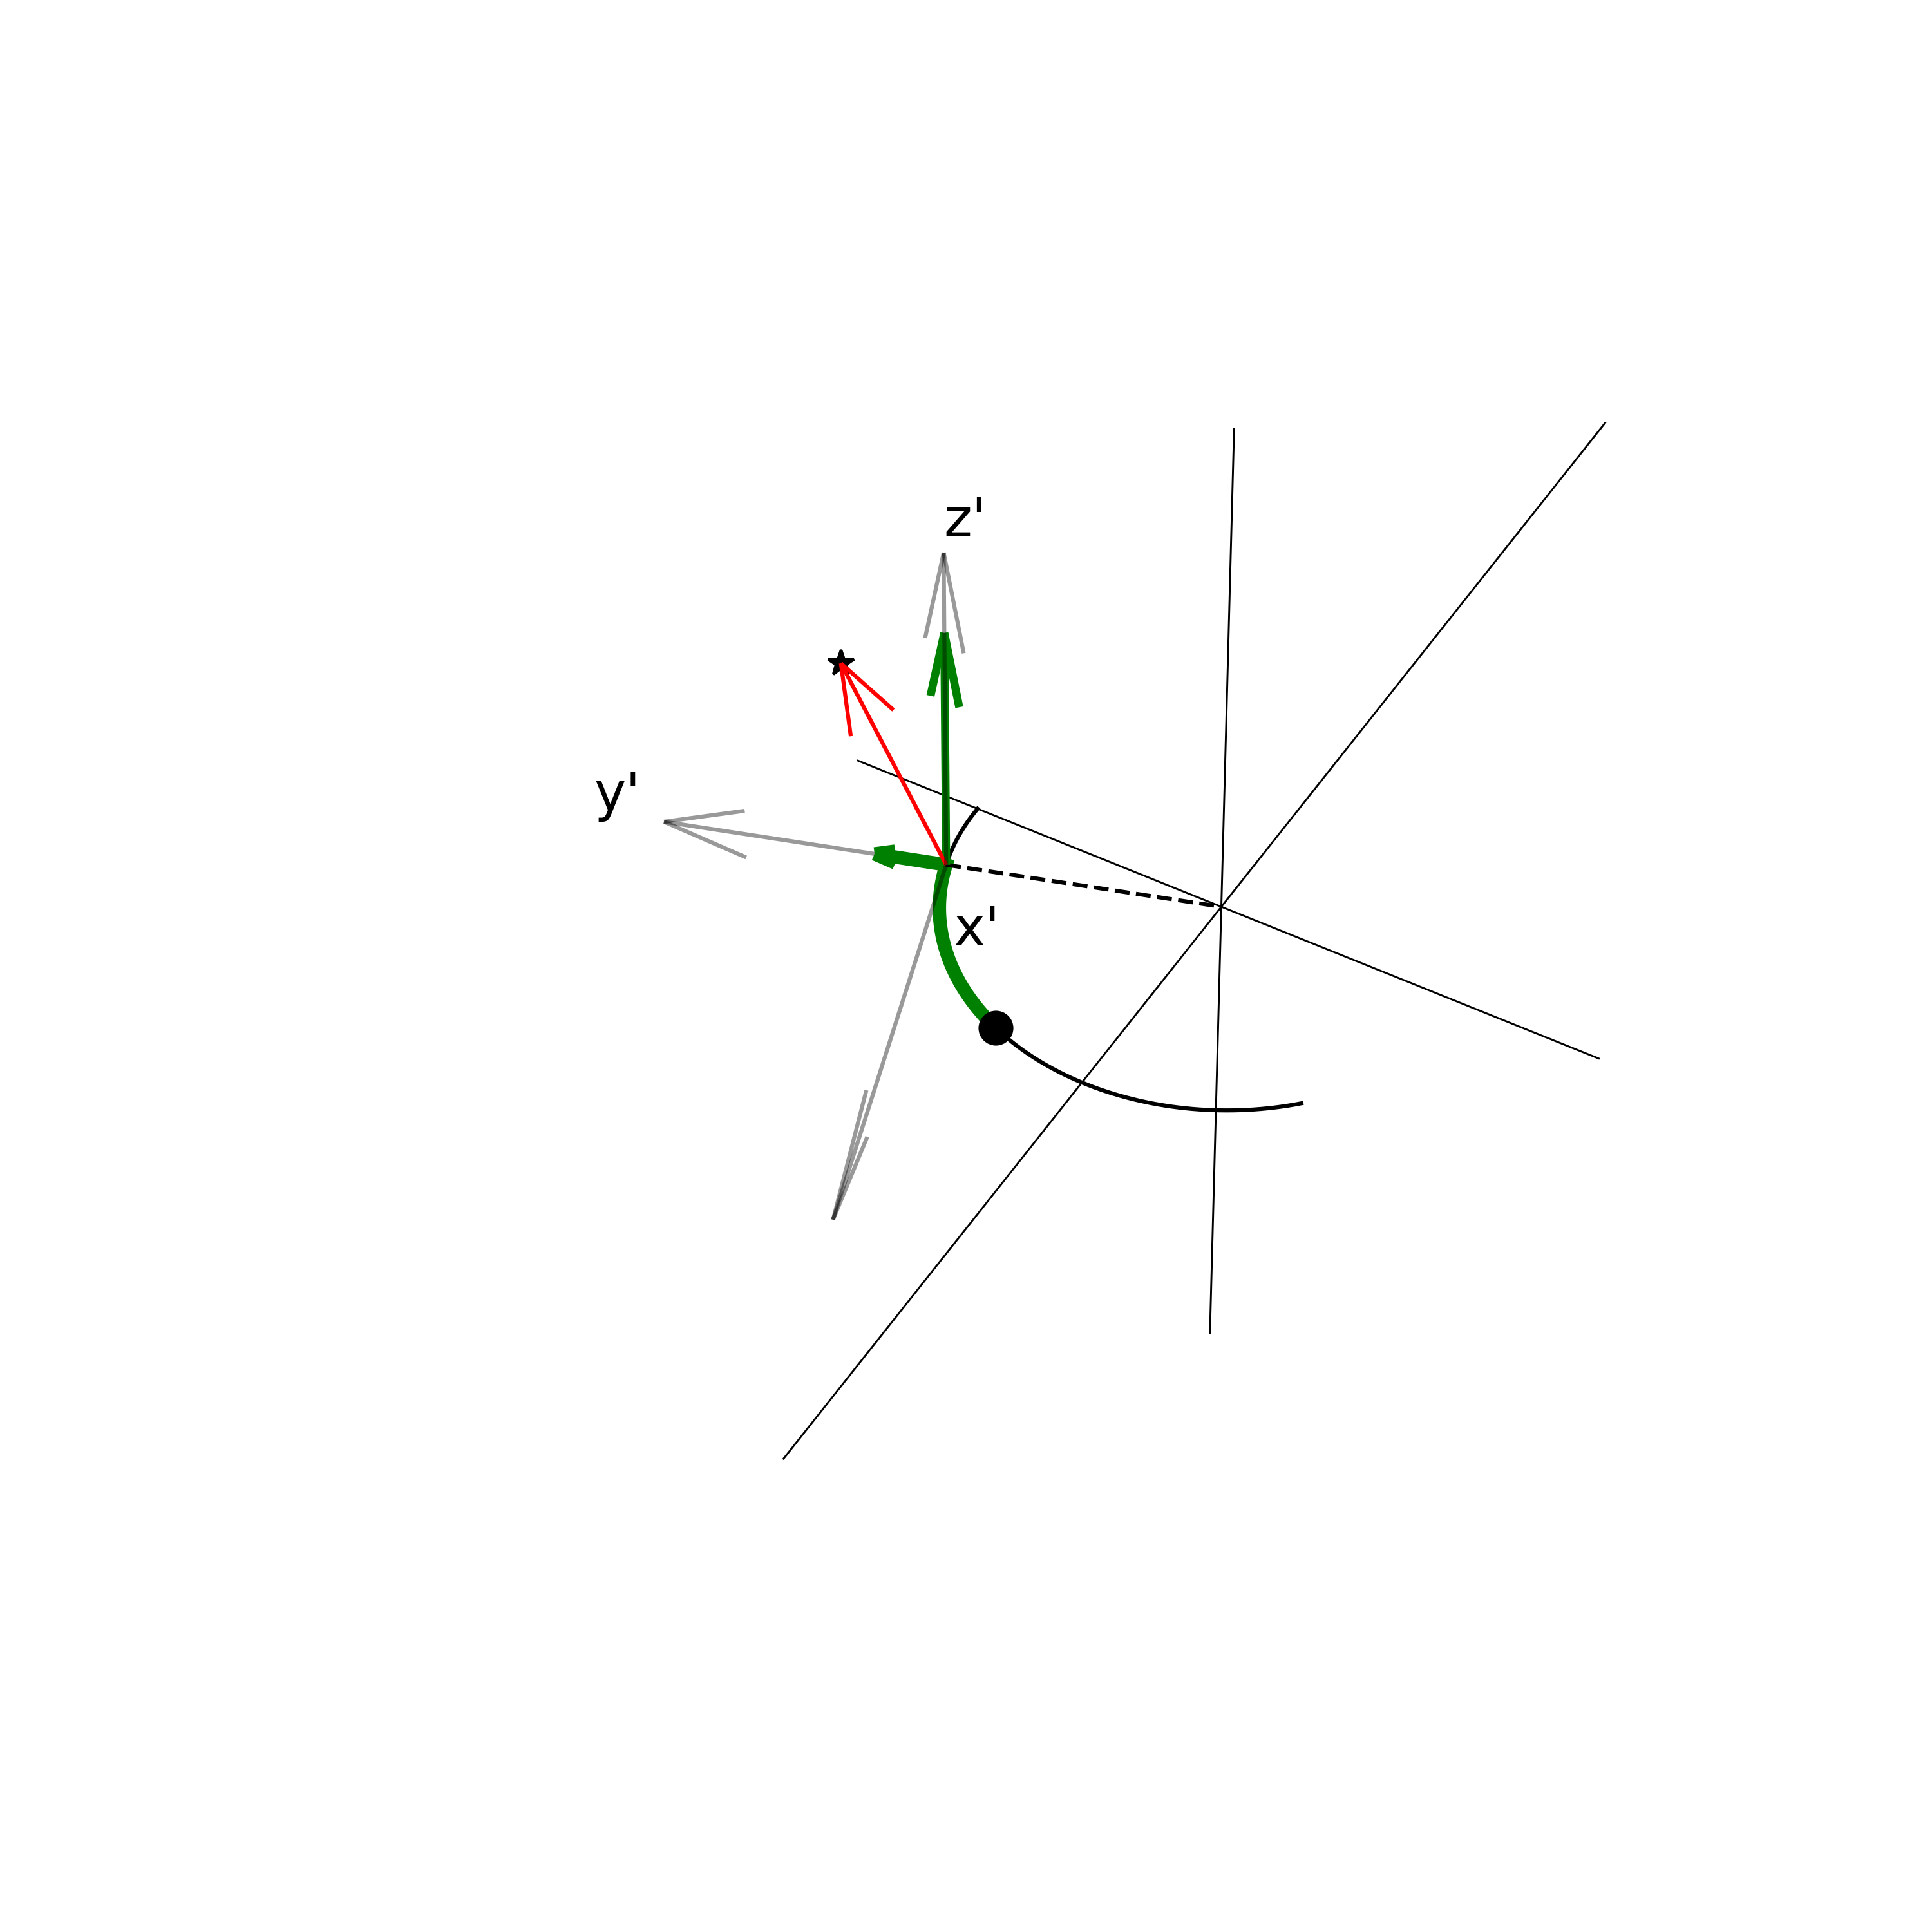
\includegraphics[width=\linewidth]{figures/along_orbit_coordinate_system-approved.png}
    \caption{Tail coordinates}
    \label{fig:TailCoordinates}
  \end{figure}

  \section{Impact Geometry Statistics}

  \begin{figure*}
    \centering
    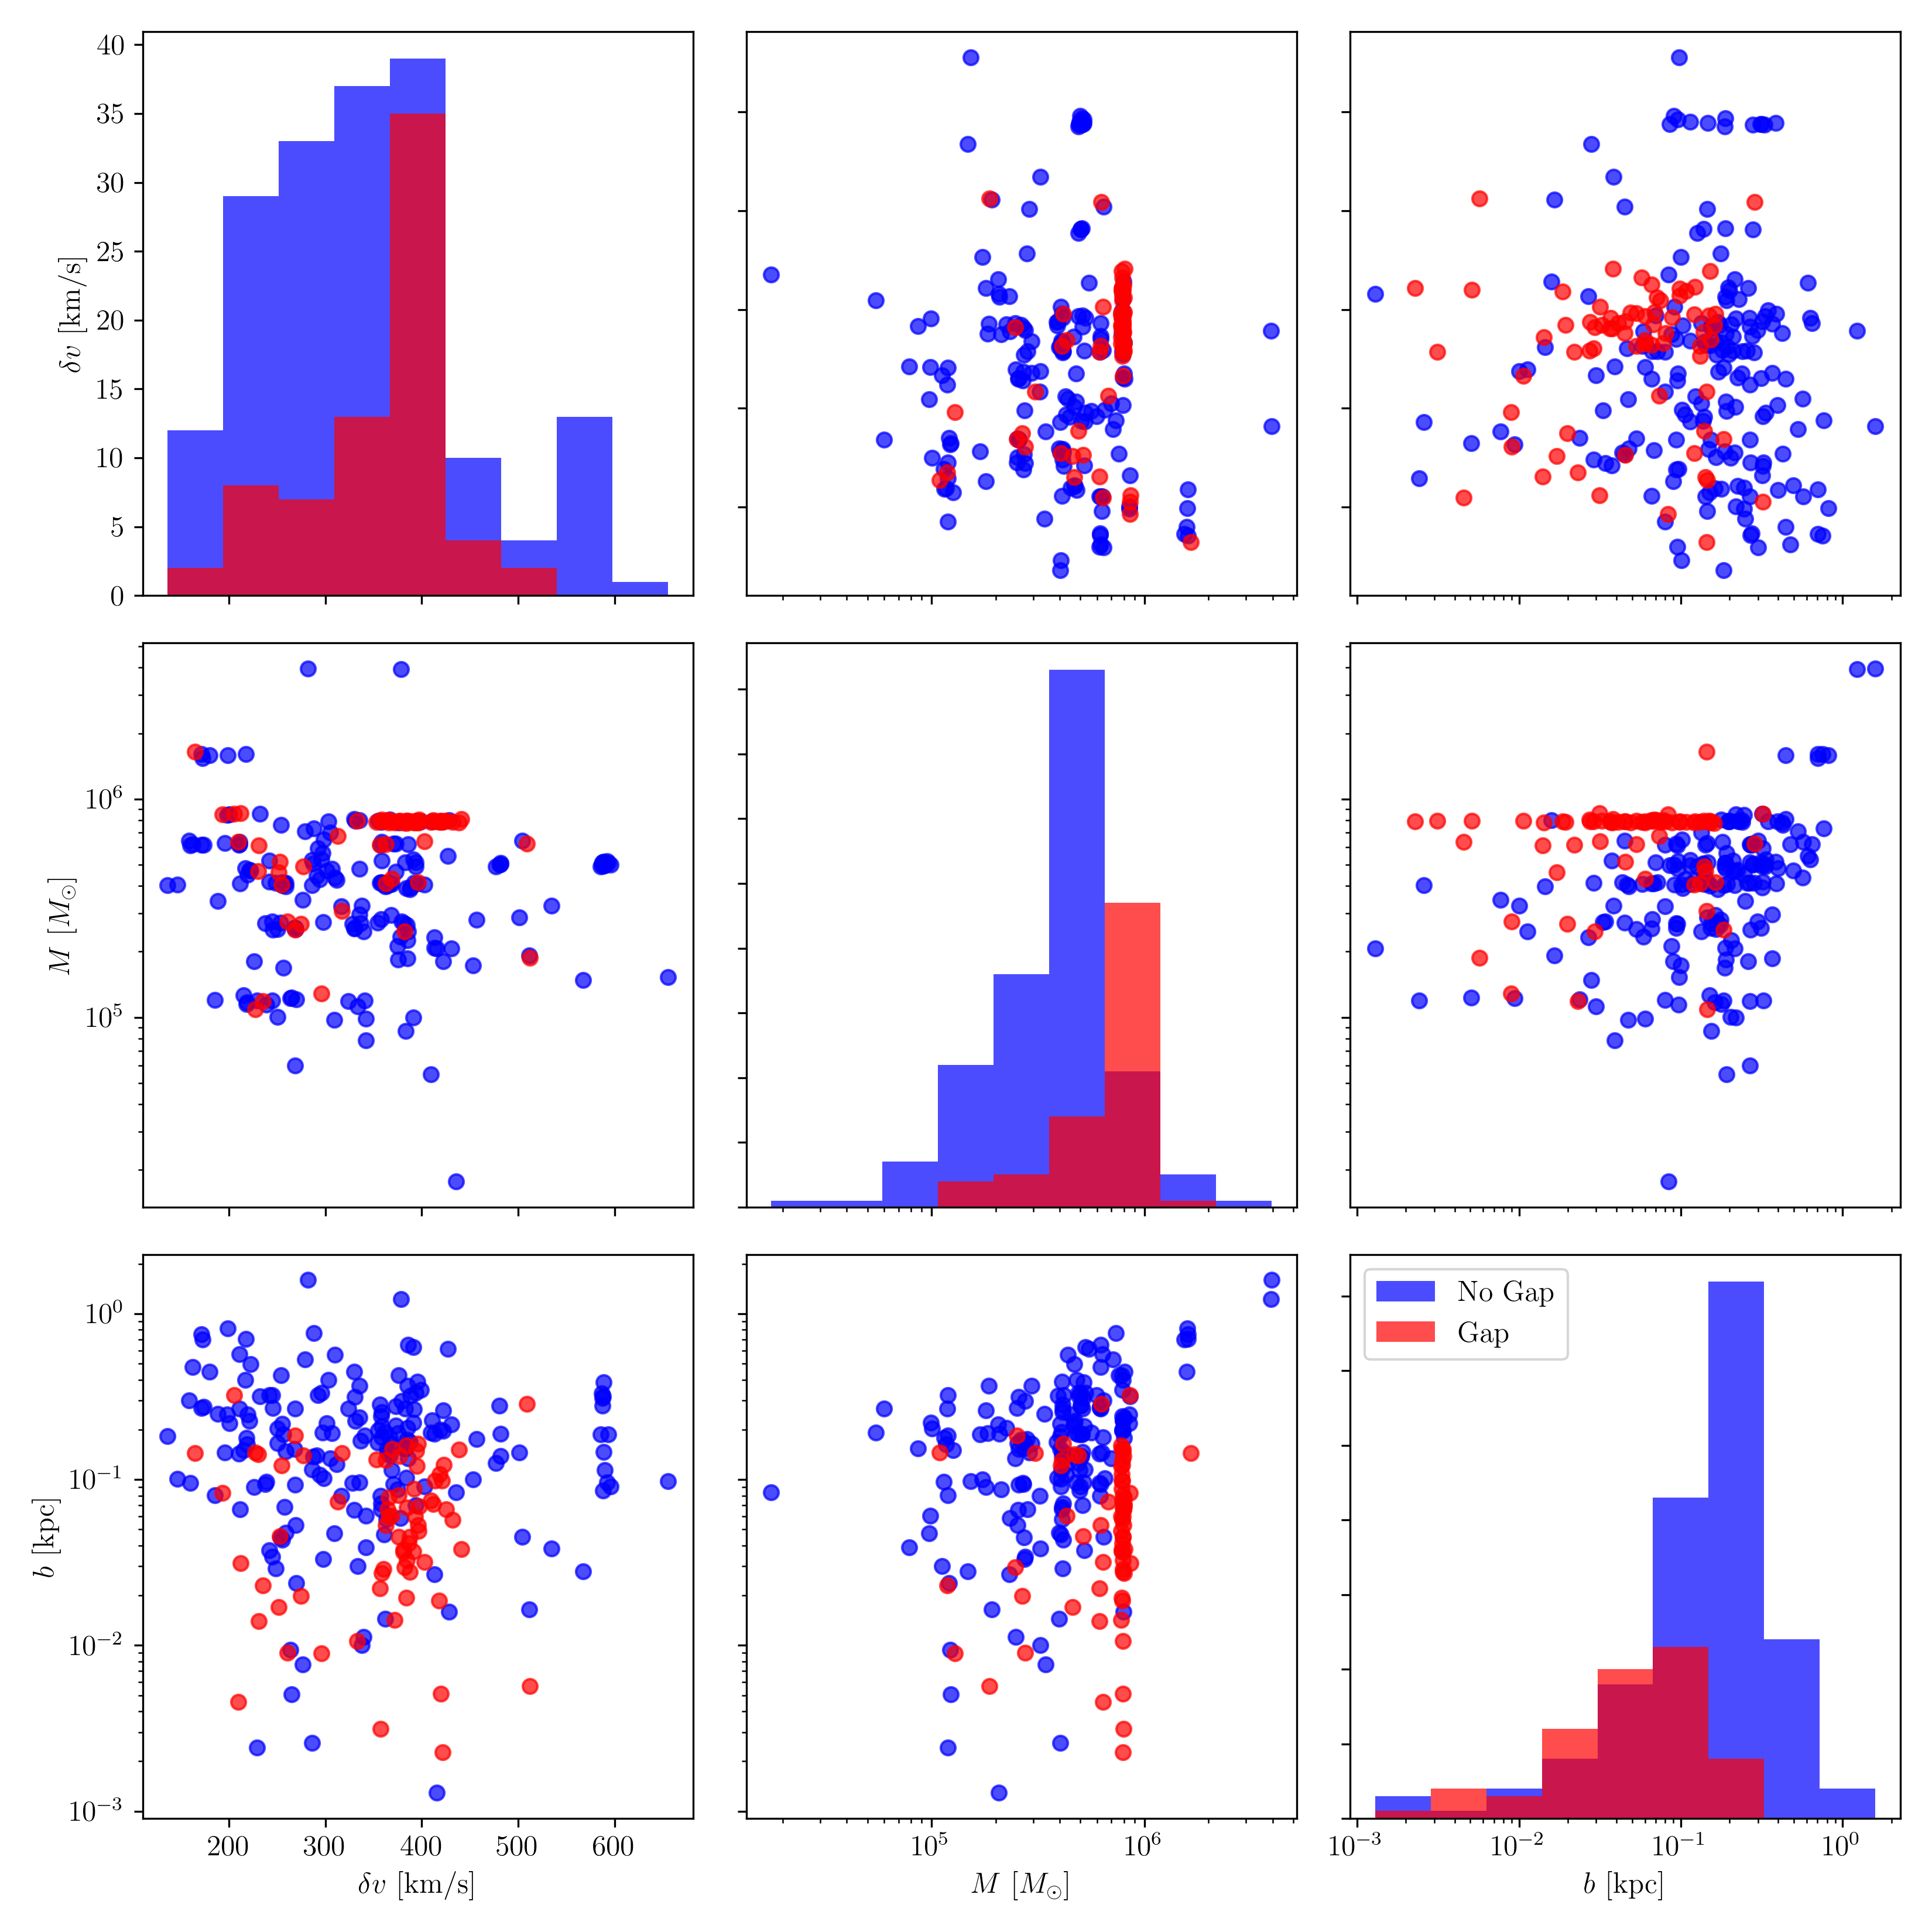
\includegraphics[width=\linewidth]{impact_geometry_statistics.png}
    \caption{Impact geometry statistics}
    \label{fig:impact_geometry_statistics}    
    \end{figure*}


  \section{Gallery of Gaps} \label{appendix:gallery_of_gaps}

    \begin{figure*}
      \centering
      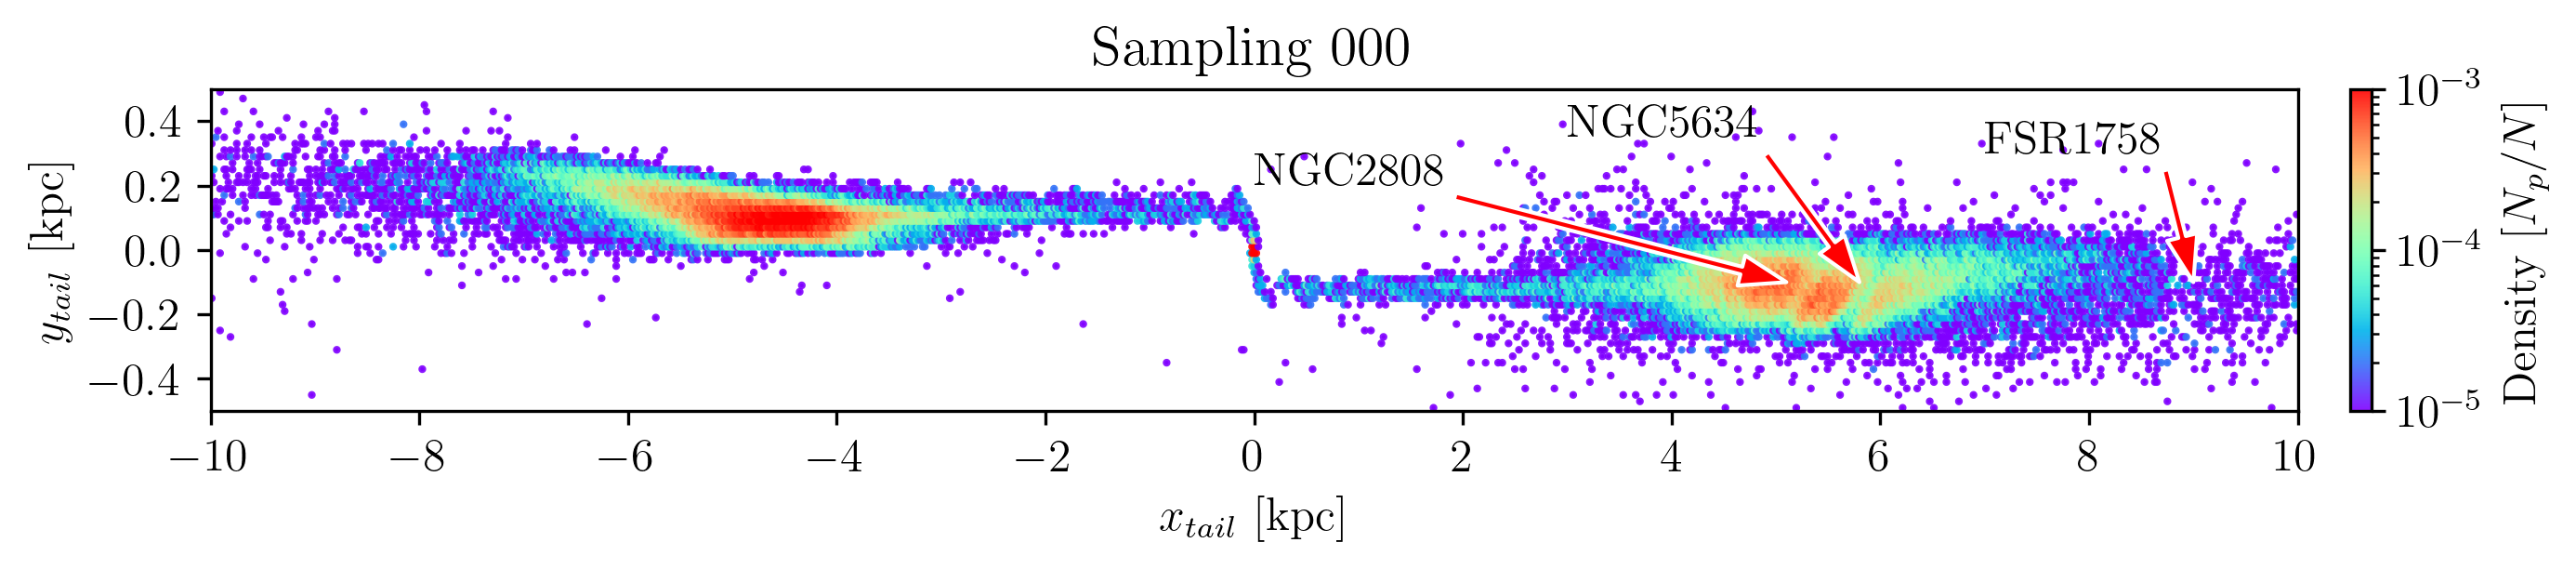
\includegraphics[width=\linewidth]{gallery_of_gaps_monte-carlo-000.png}
      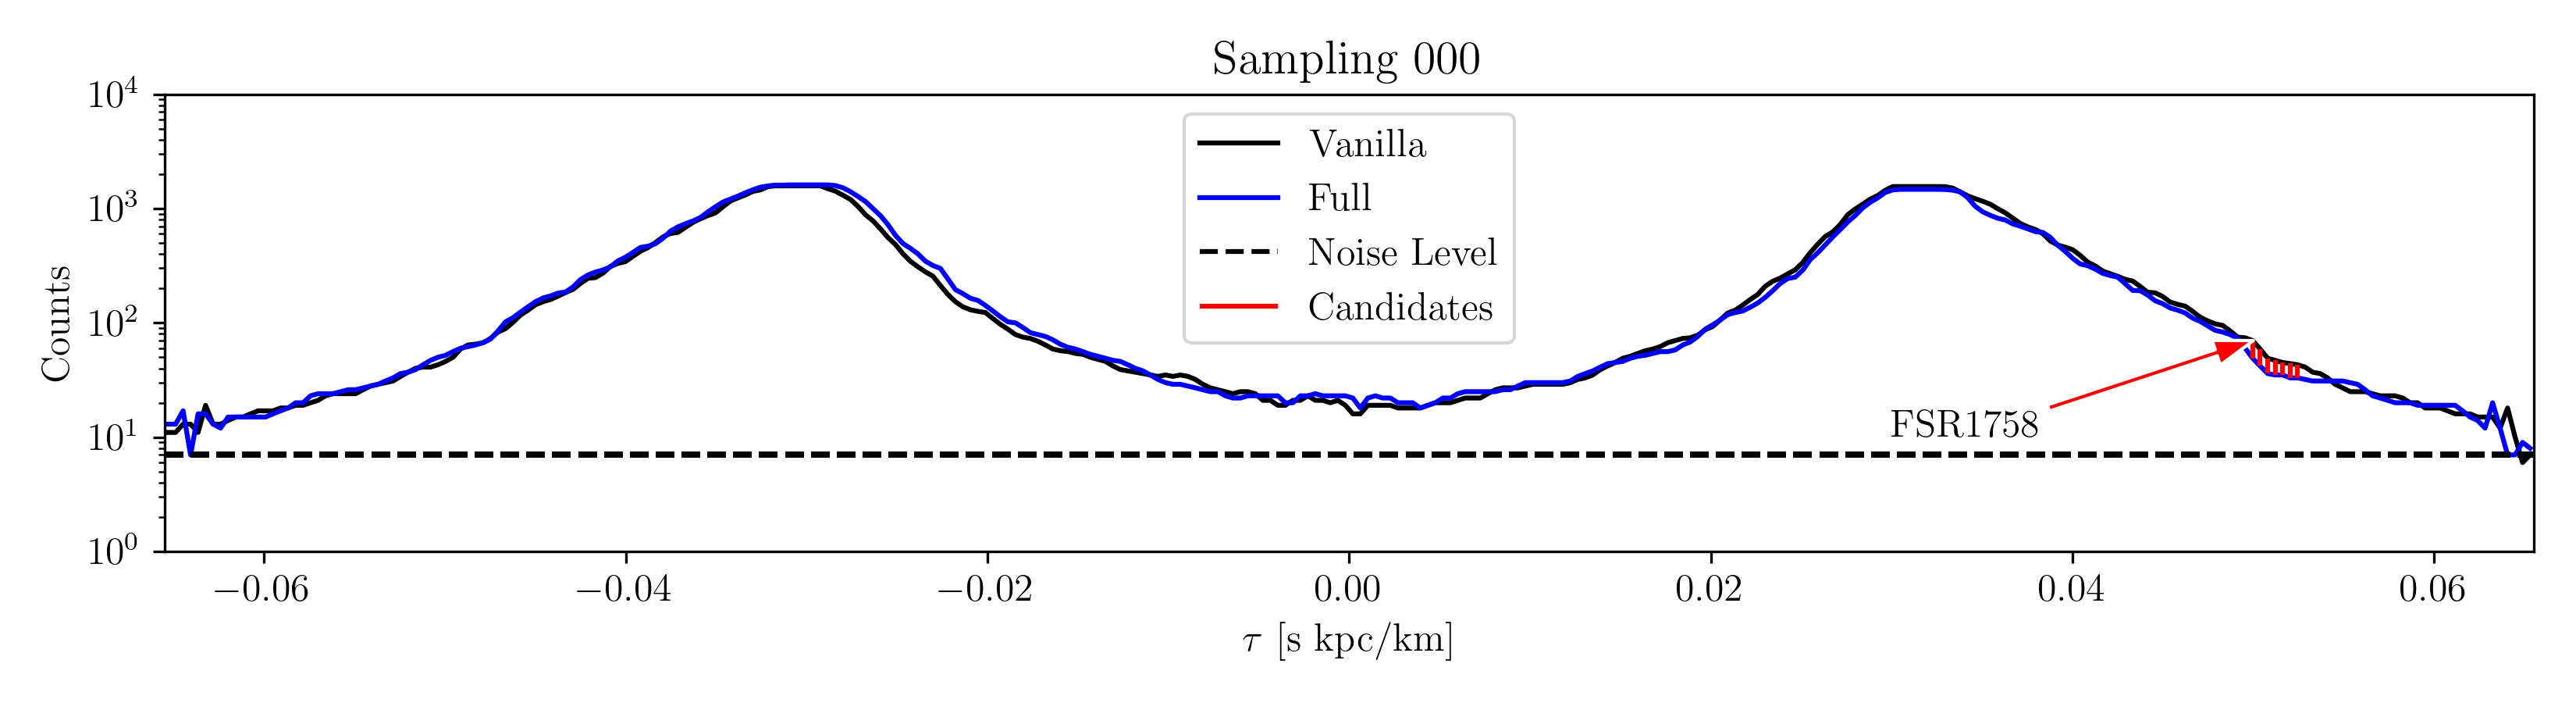
\includegraphics[width=\linewidth]{tau-profile-monte-carlo-000.png}
      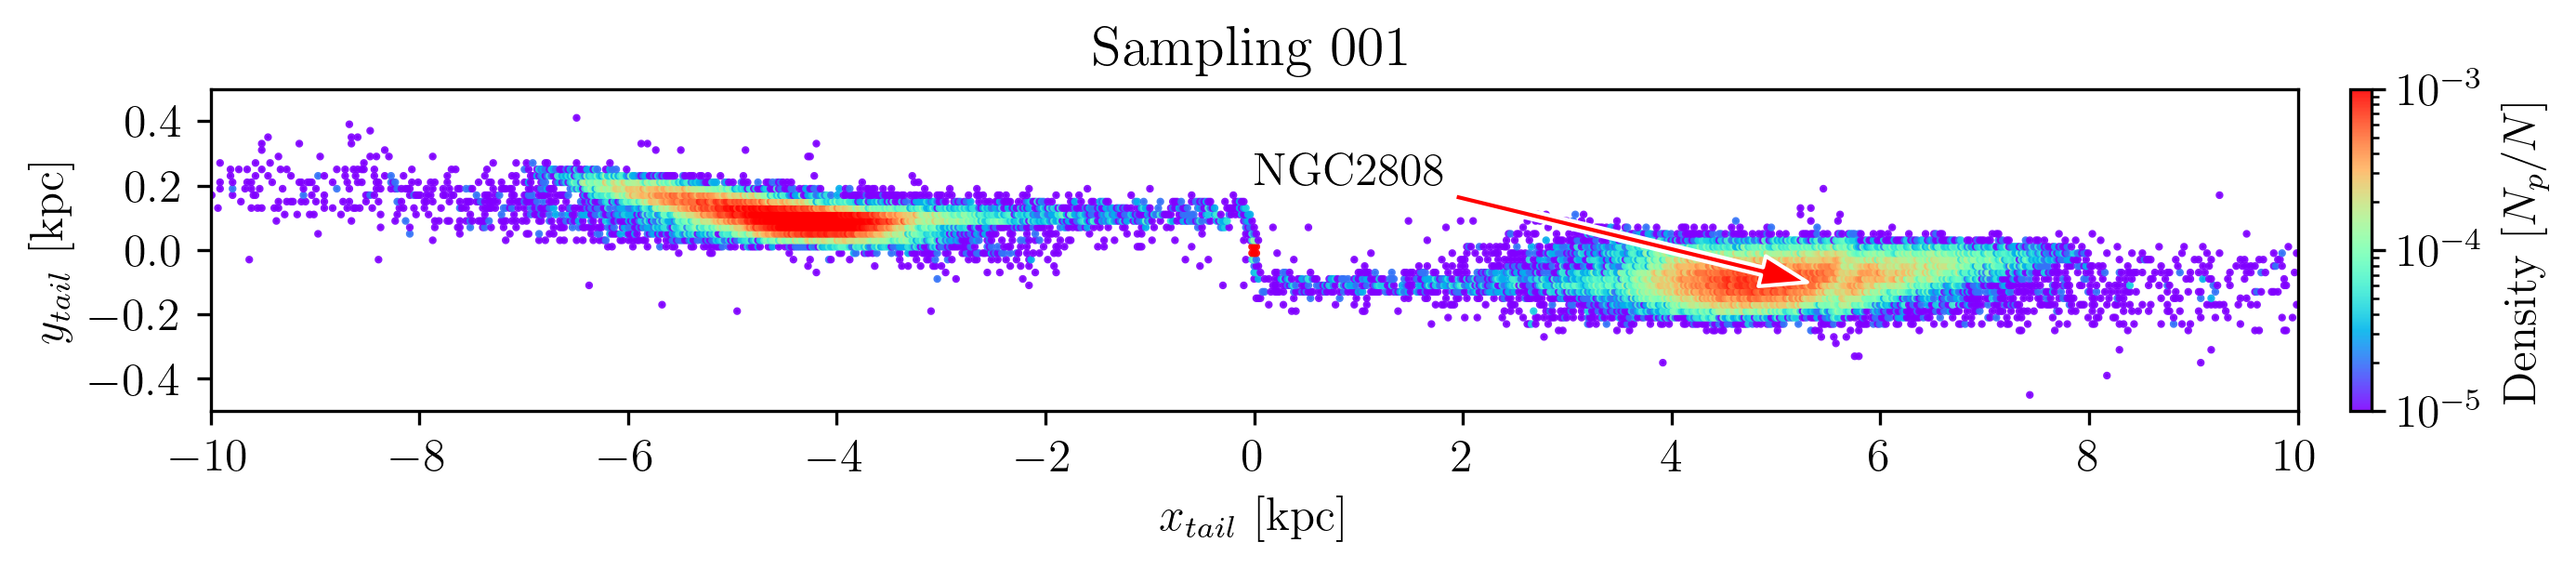
\includegraphics[width=\linewidth]{gallery_of_gaps_monte-carlo-001.png}
      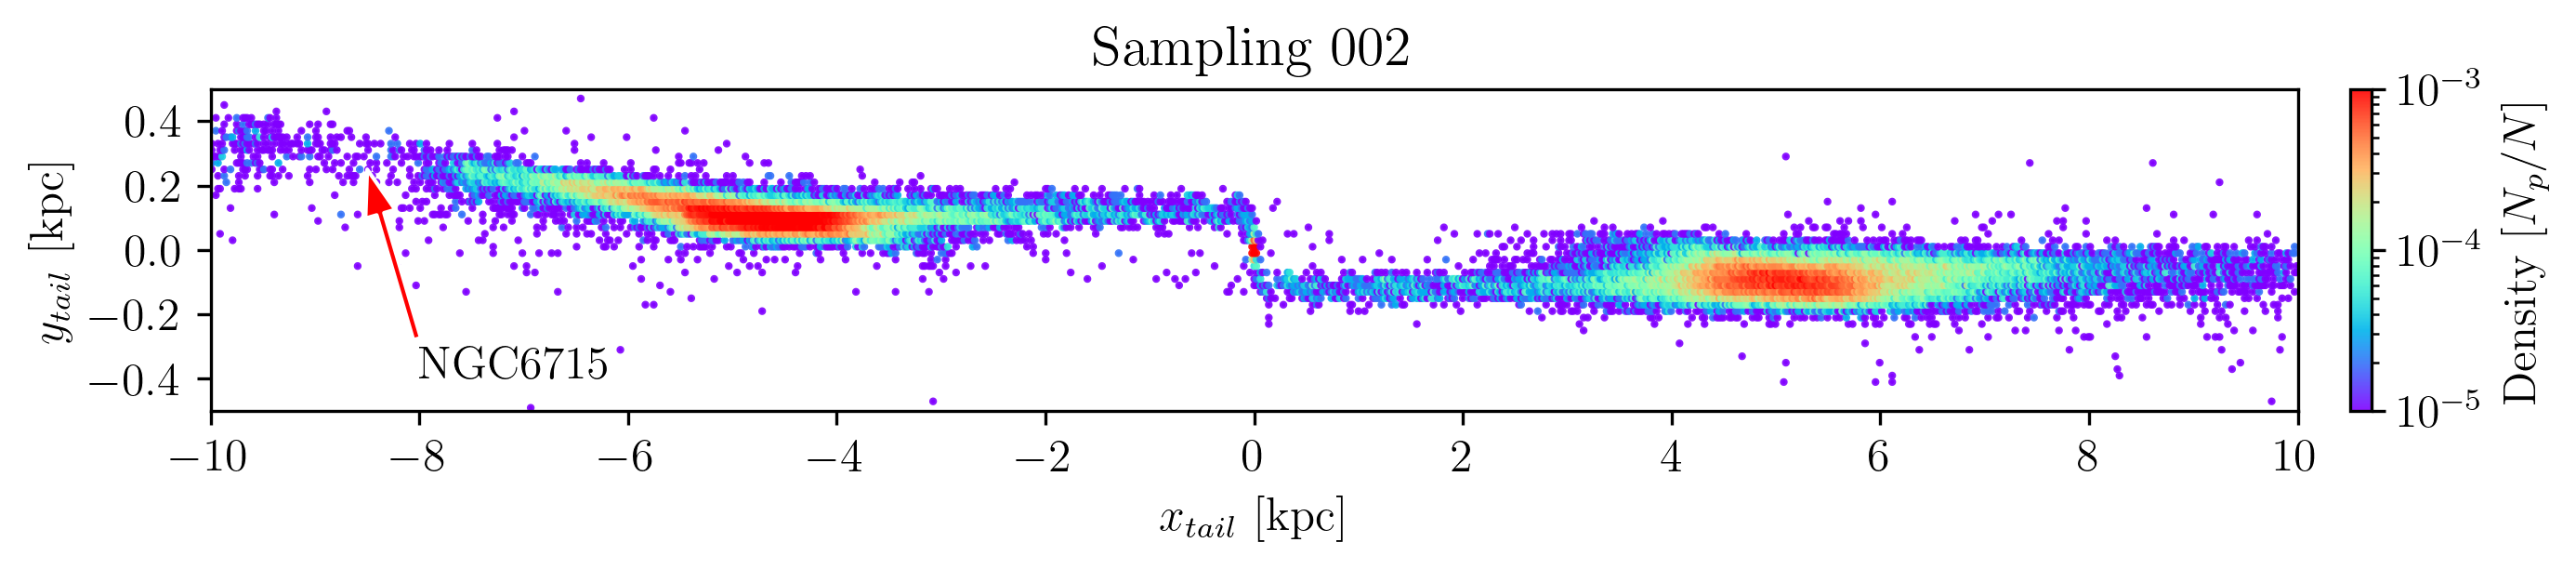
\includegraphics[width=\linewidth]{gallery_of_gaps_monte-carlo-002.png}
      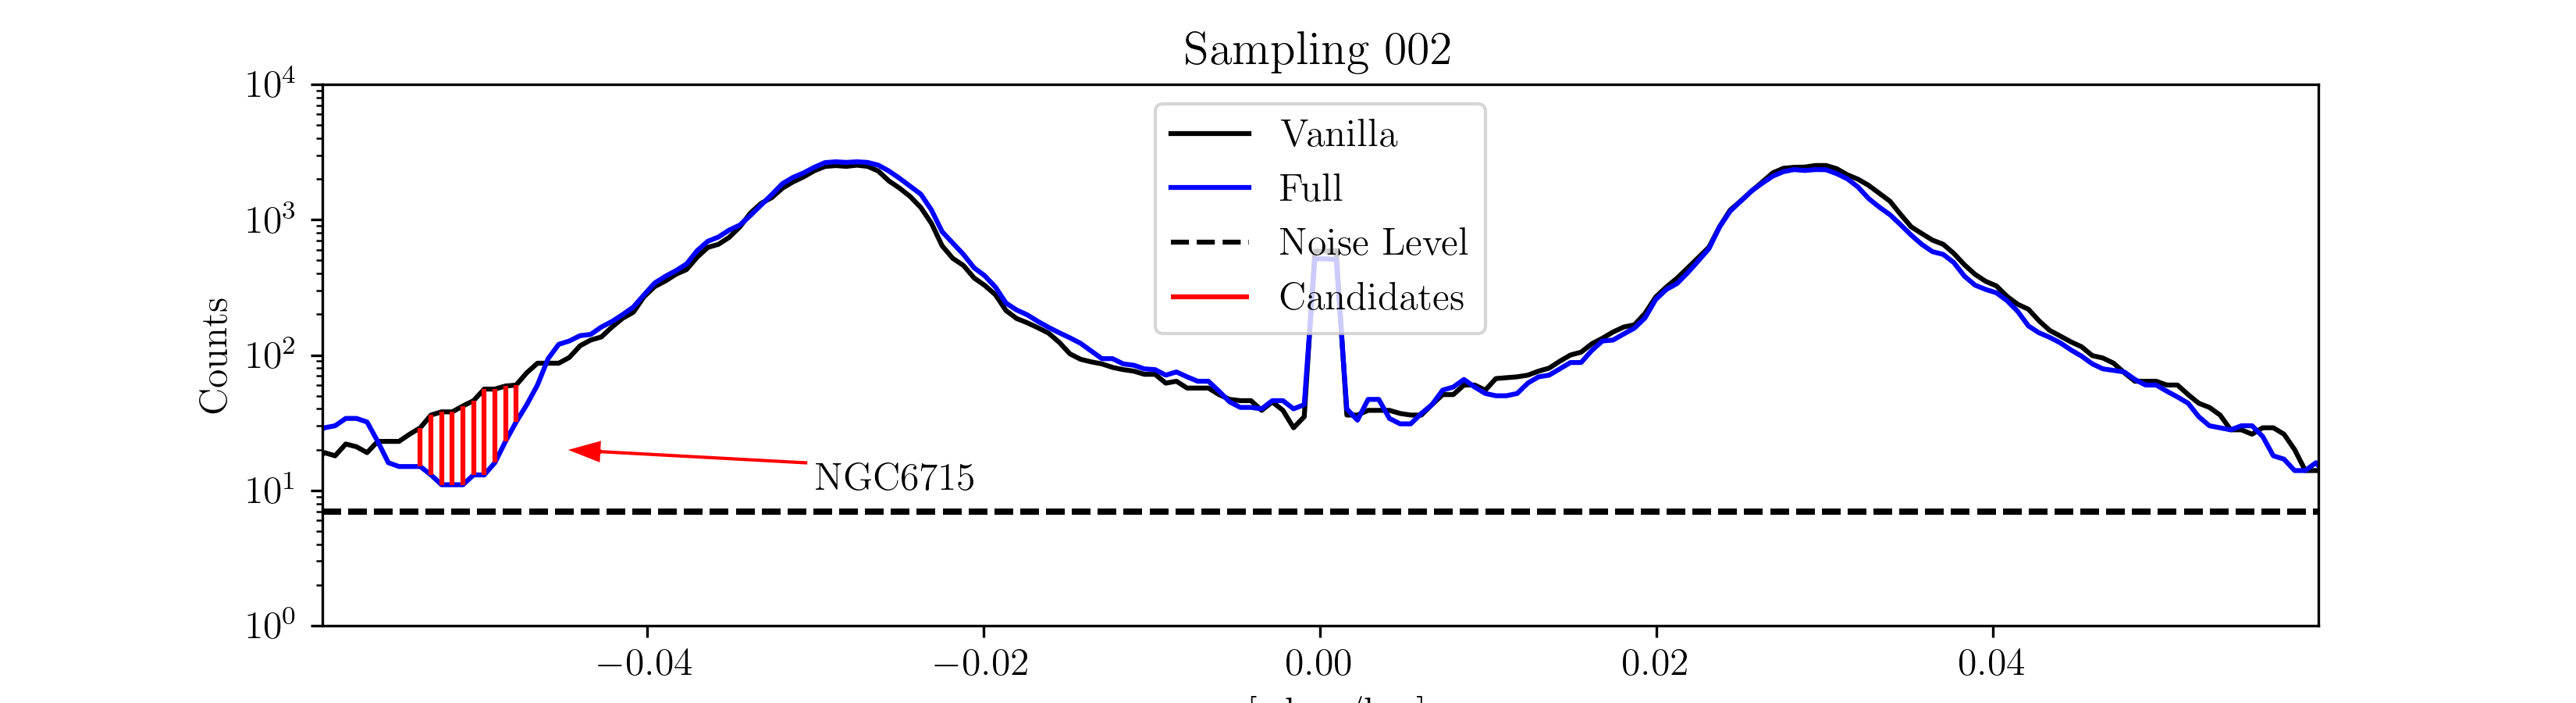
\includegraphics[width=\linewidth]{tau-profile-monte-carlo-002.png}
      \caption{Gap Gallery}
      \label{fig:TailCoordinates}
    \end{figure*}    


    \begin{figure*}
      \centering
      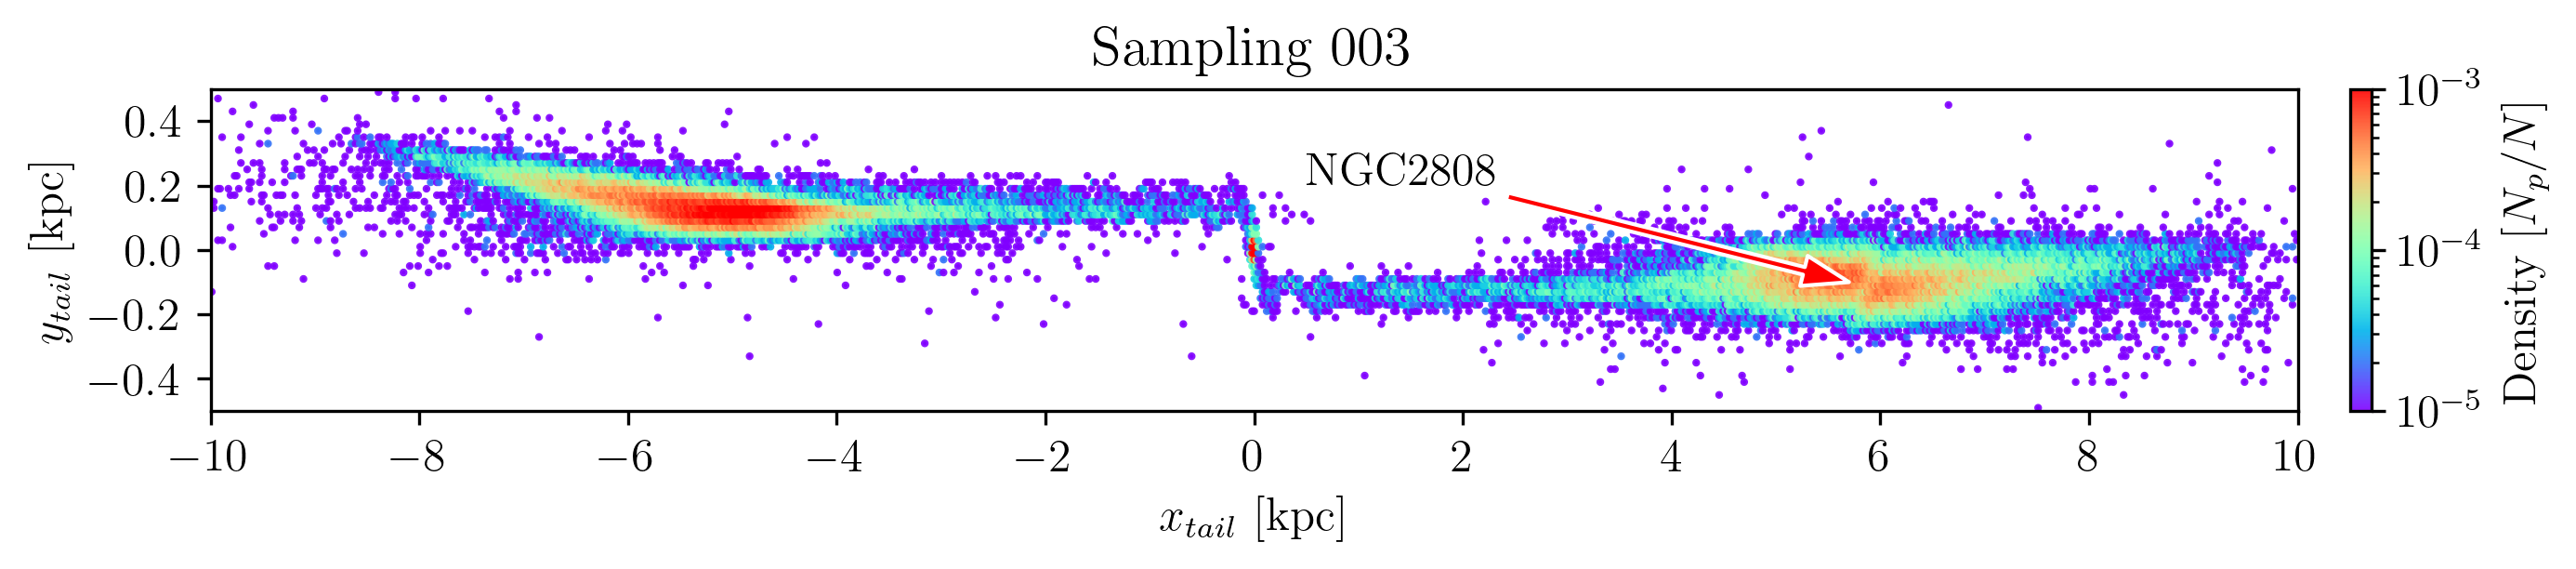
\includegraphics[width=\linewidth]{gallery_of_gaps_monte-carlo-003.png}      
      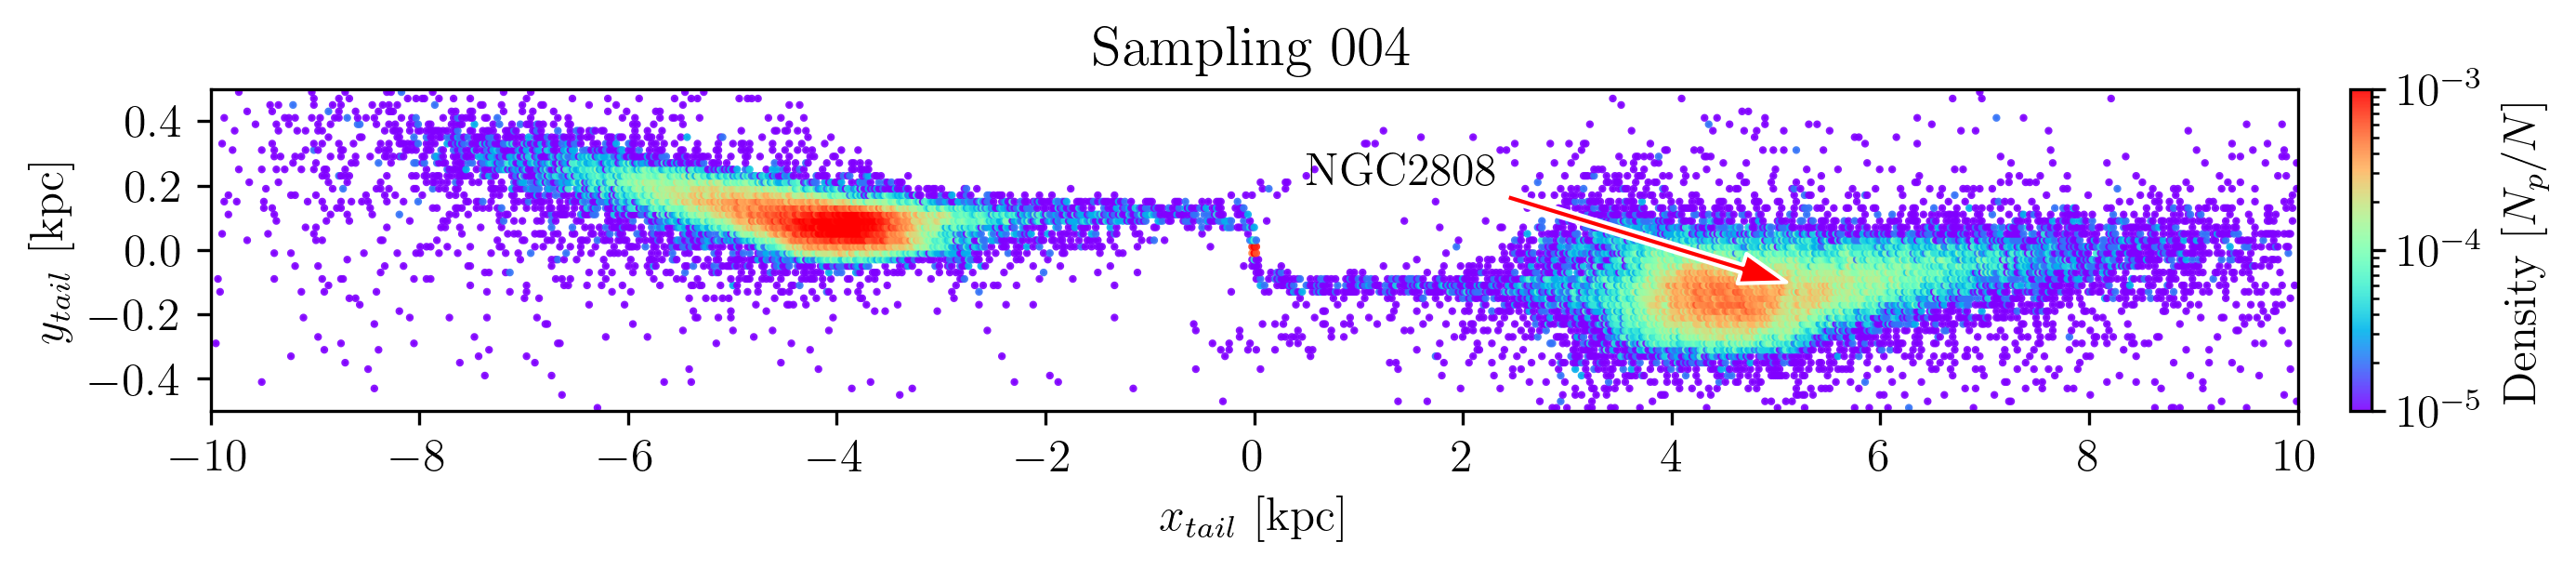
\includegraphics[width=\linewidth]{gallery_of_gaps_monte-carlo-004.png}
      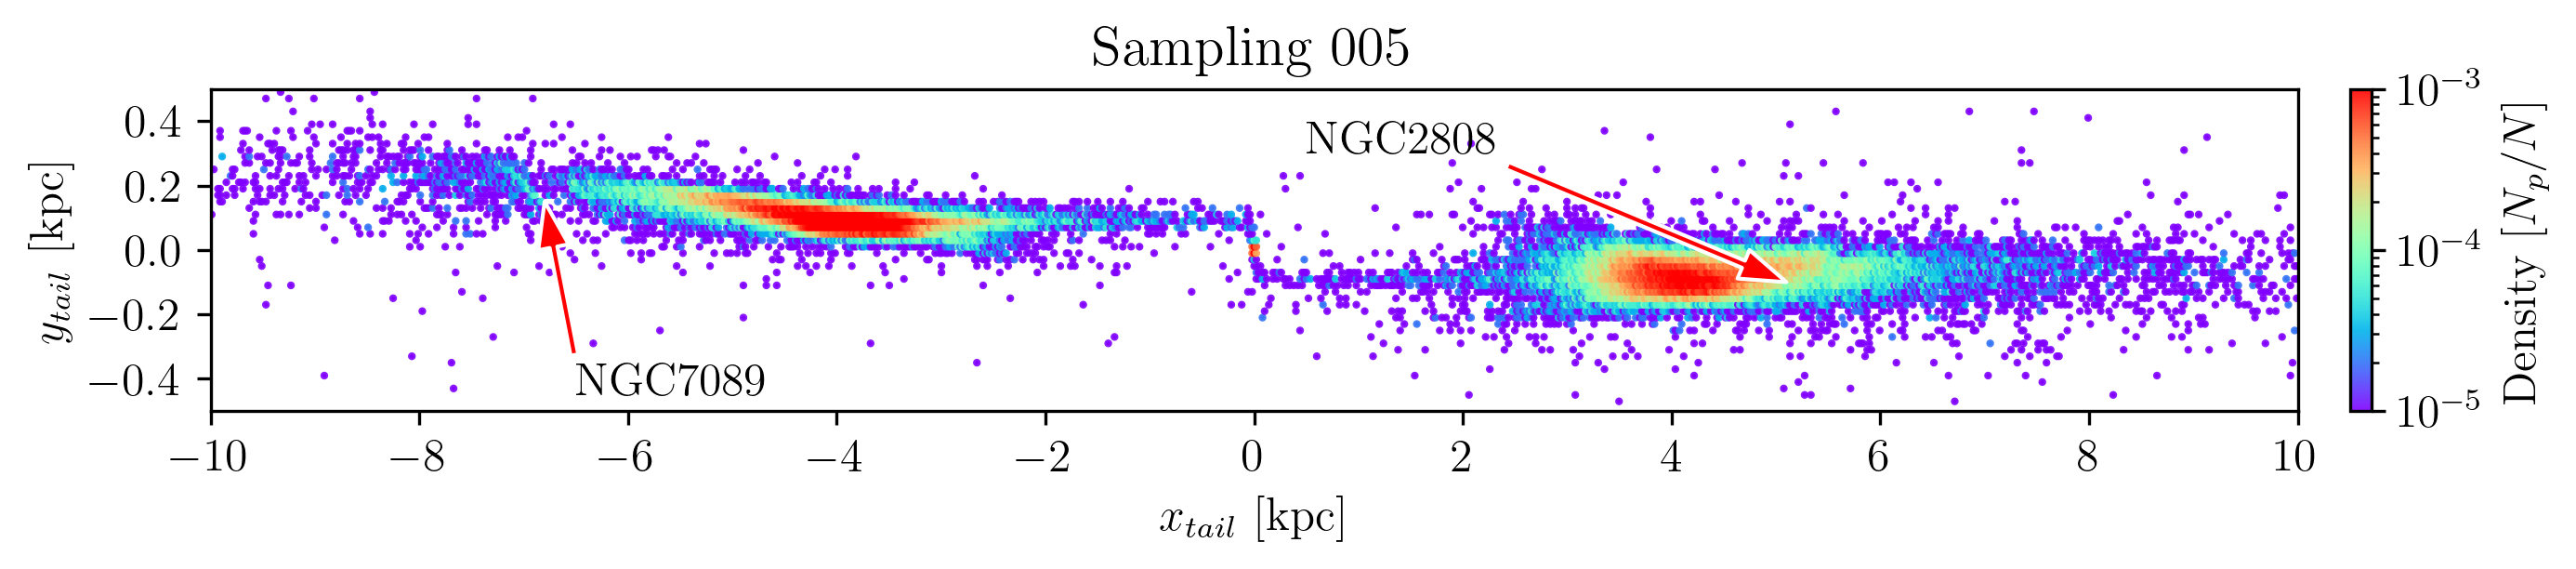
\includegraphics[width=\linewidth]{gallery_of_gaps_monte-carlo-005.png}
      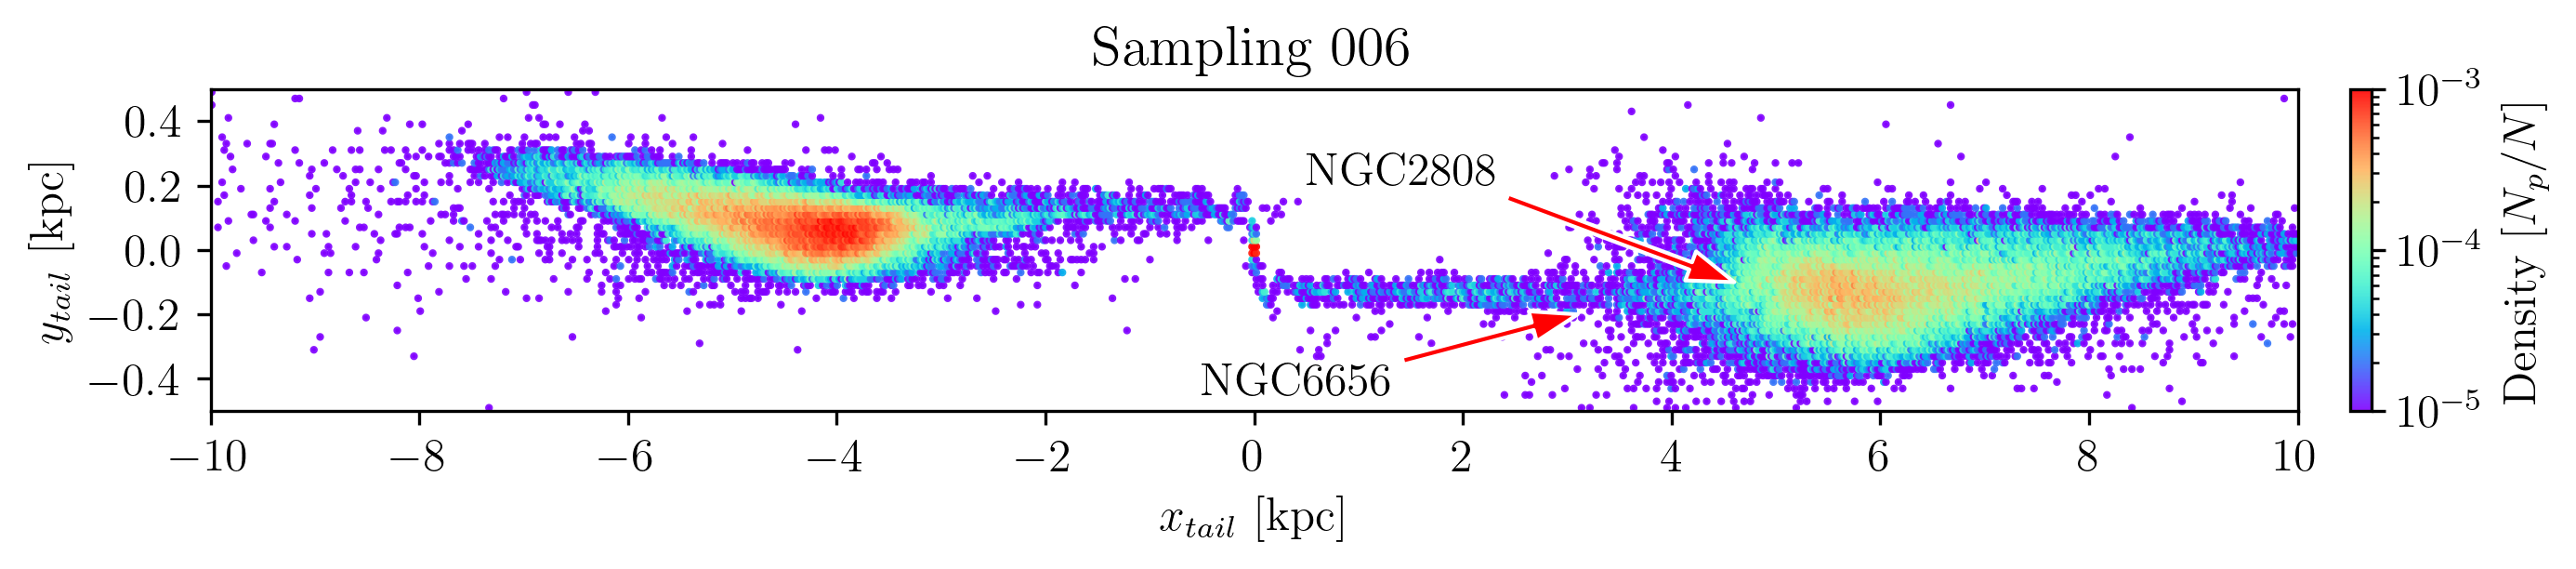
\includegraphics[width=\linewidth]{gallery_of_gaps_monte-carlo-006.png}
      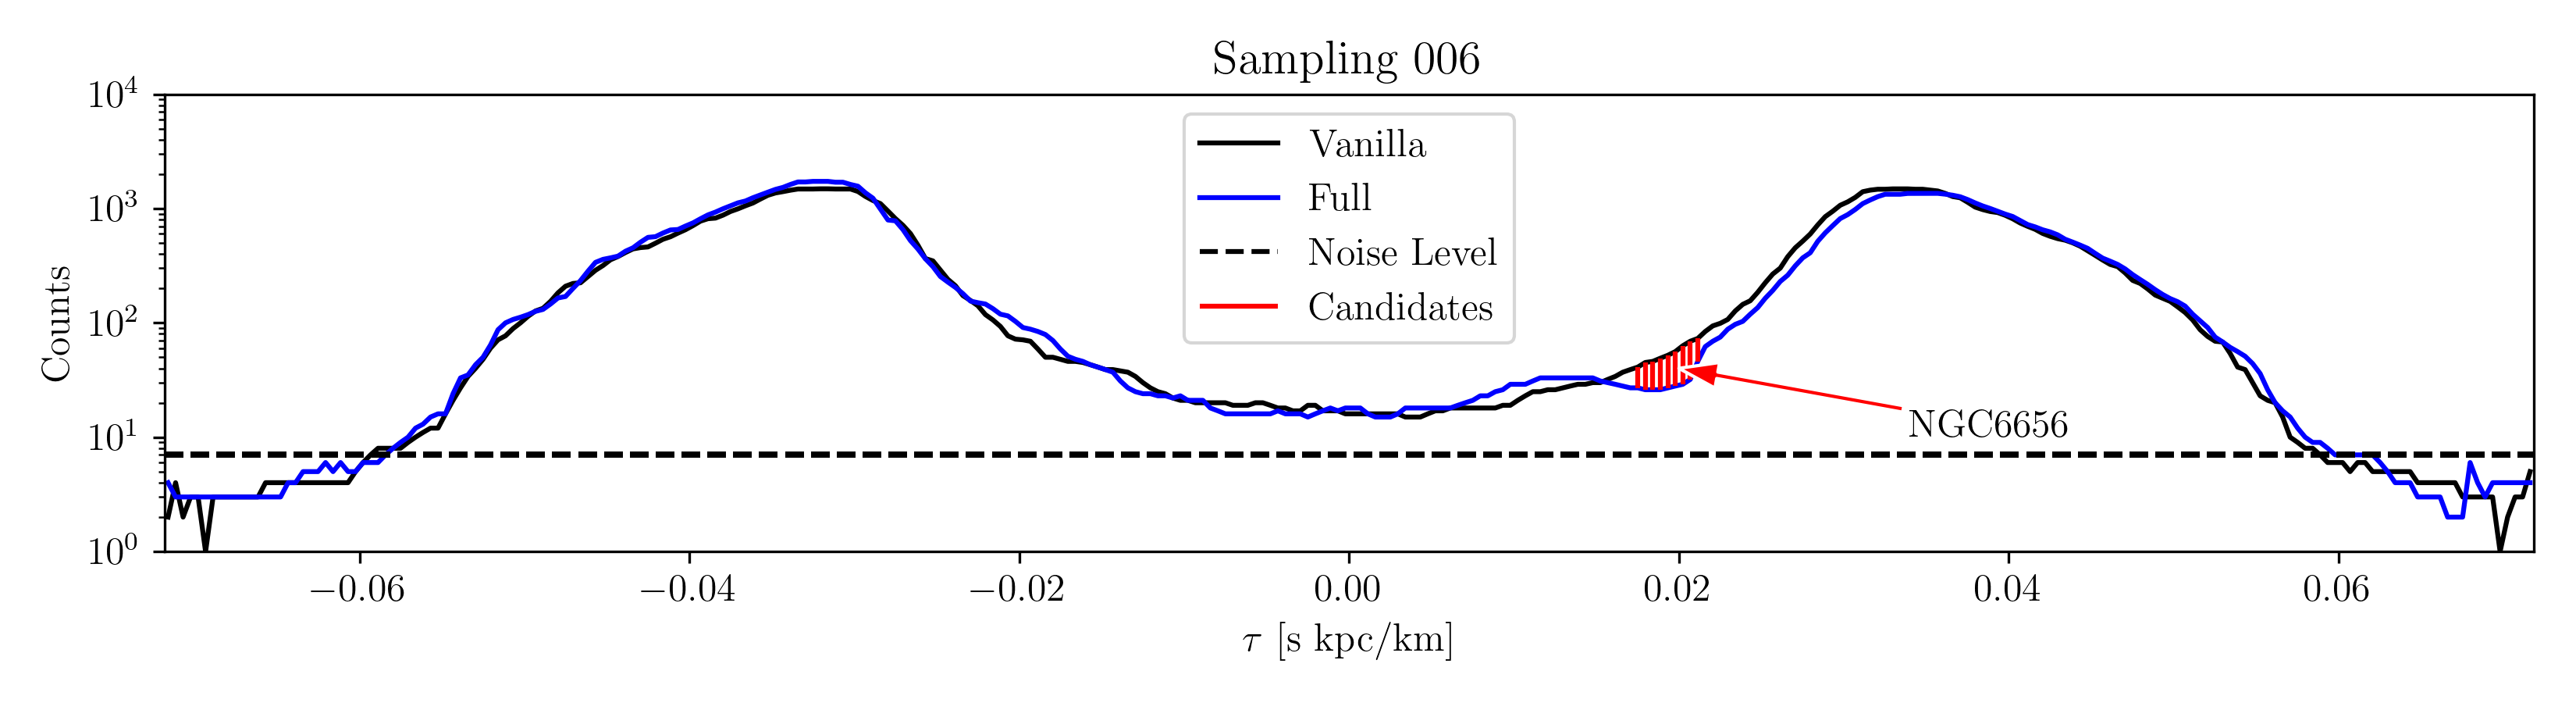
\includegraphics[width=\linewidth]{tau-profile-monte-carlo-006.png}
      \caption{Gap Gallery}
      \label{fig:TailCoordinates}
    \end{figure*}        


    \begin{figure*}
      \centering
      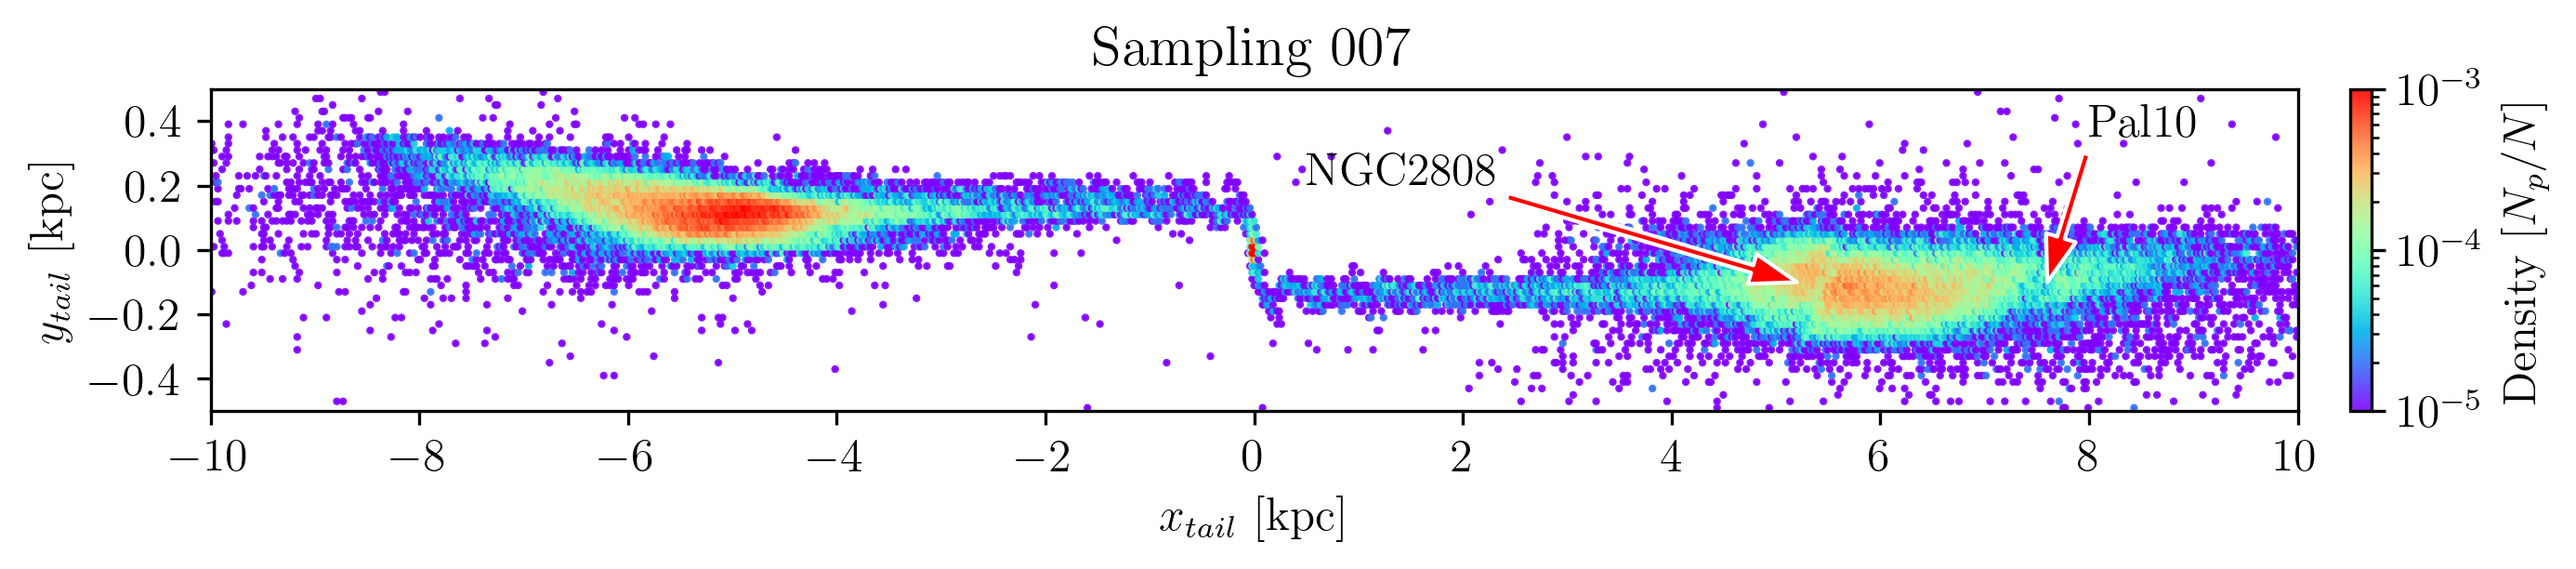
\includegraphics[width=\linewidth]{gallery_of_gaps_monte-carlo-007.png}
      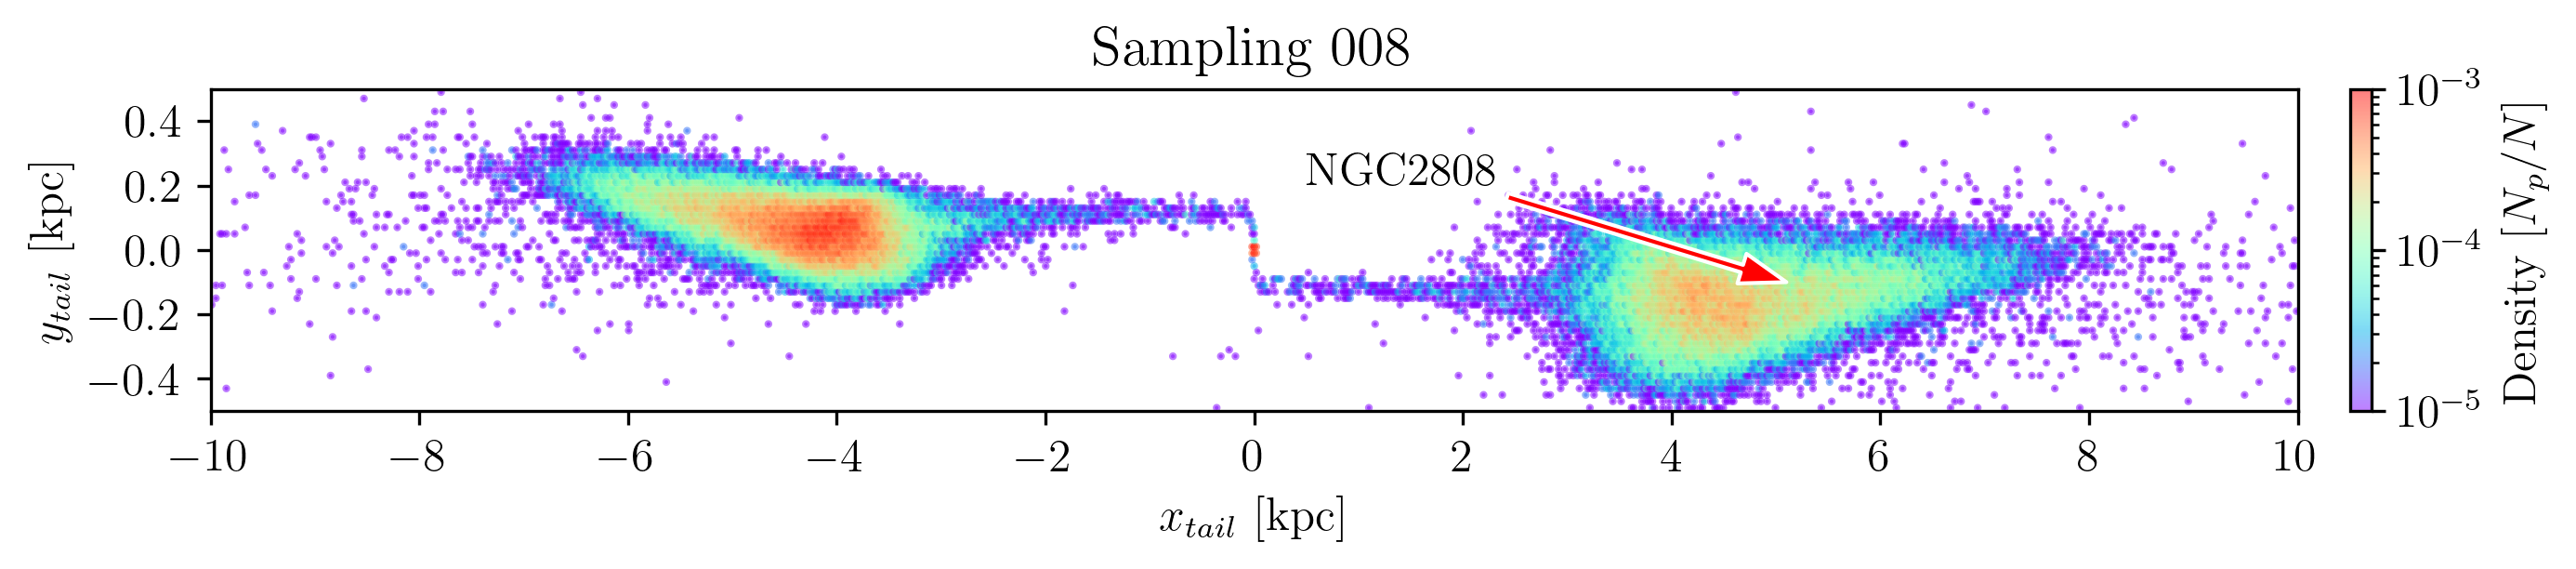
\includegraphics[width=\linewidth]{gallery_of_gaps_monte-carlo-008.png}
      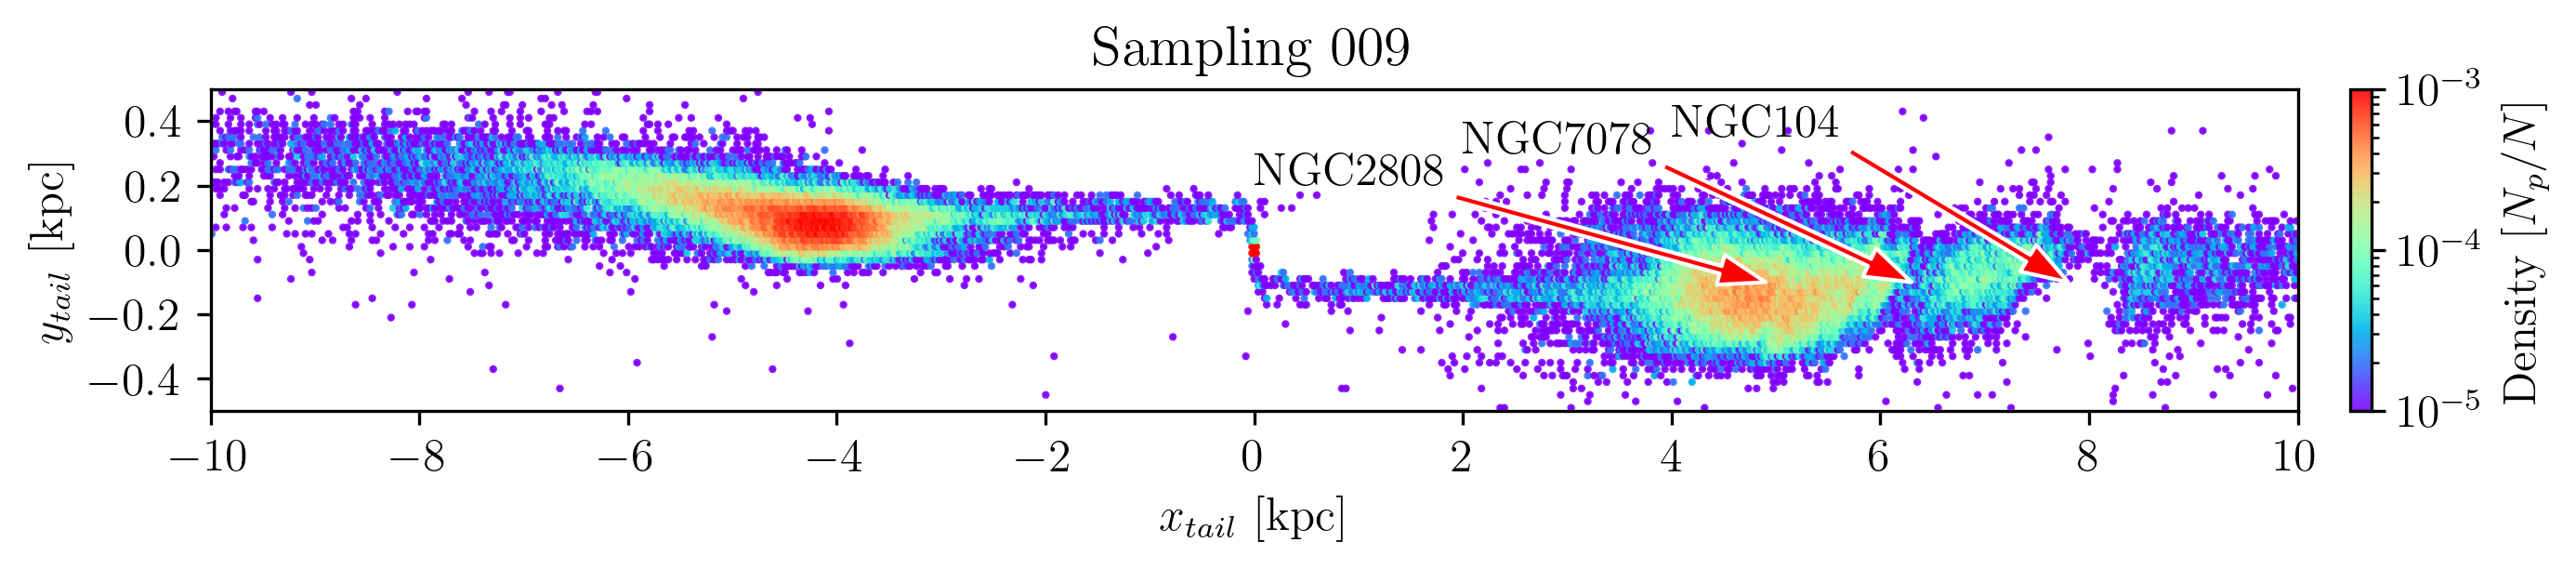
\includegraphics[width=\linewidth]{gallery_of_gaps_monte-carlo-009.png}      
      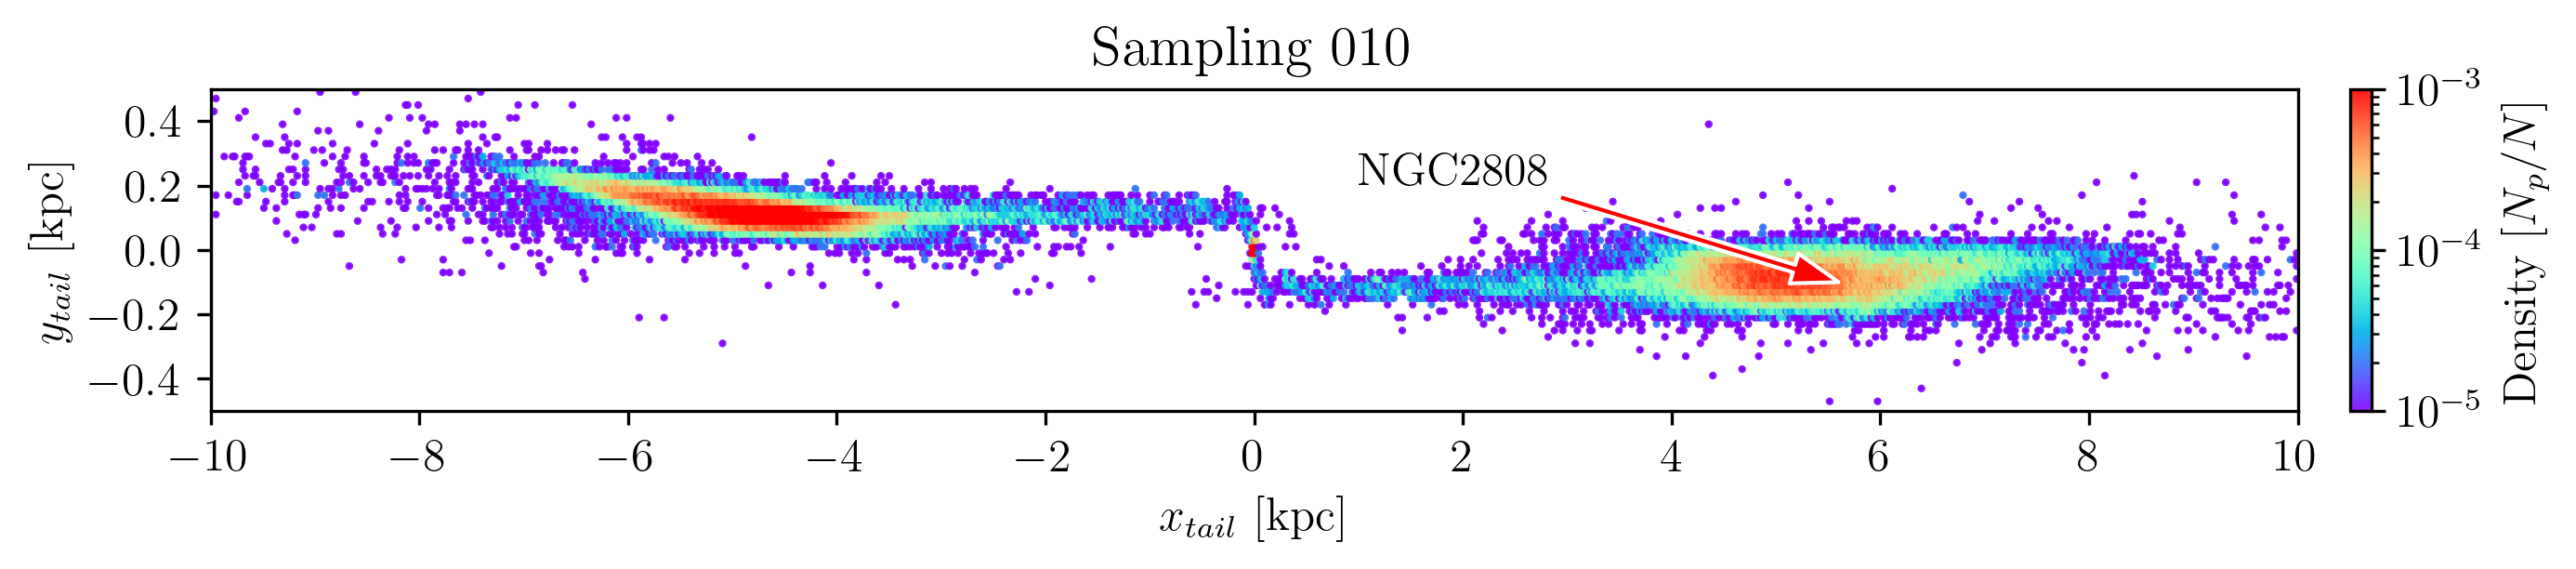
\includegraphics[width=\linewidth]{gallery_of_gaps_monte-carlo-010.png}
      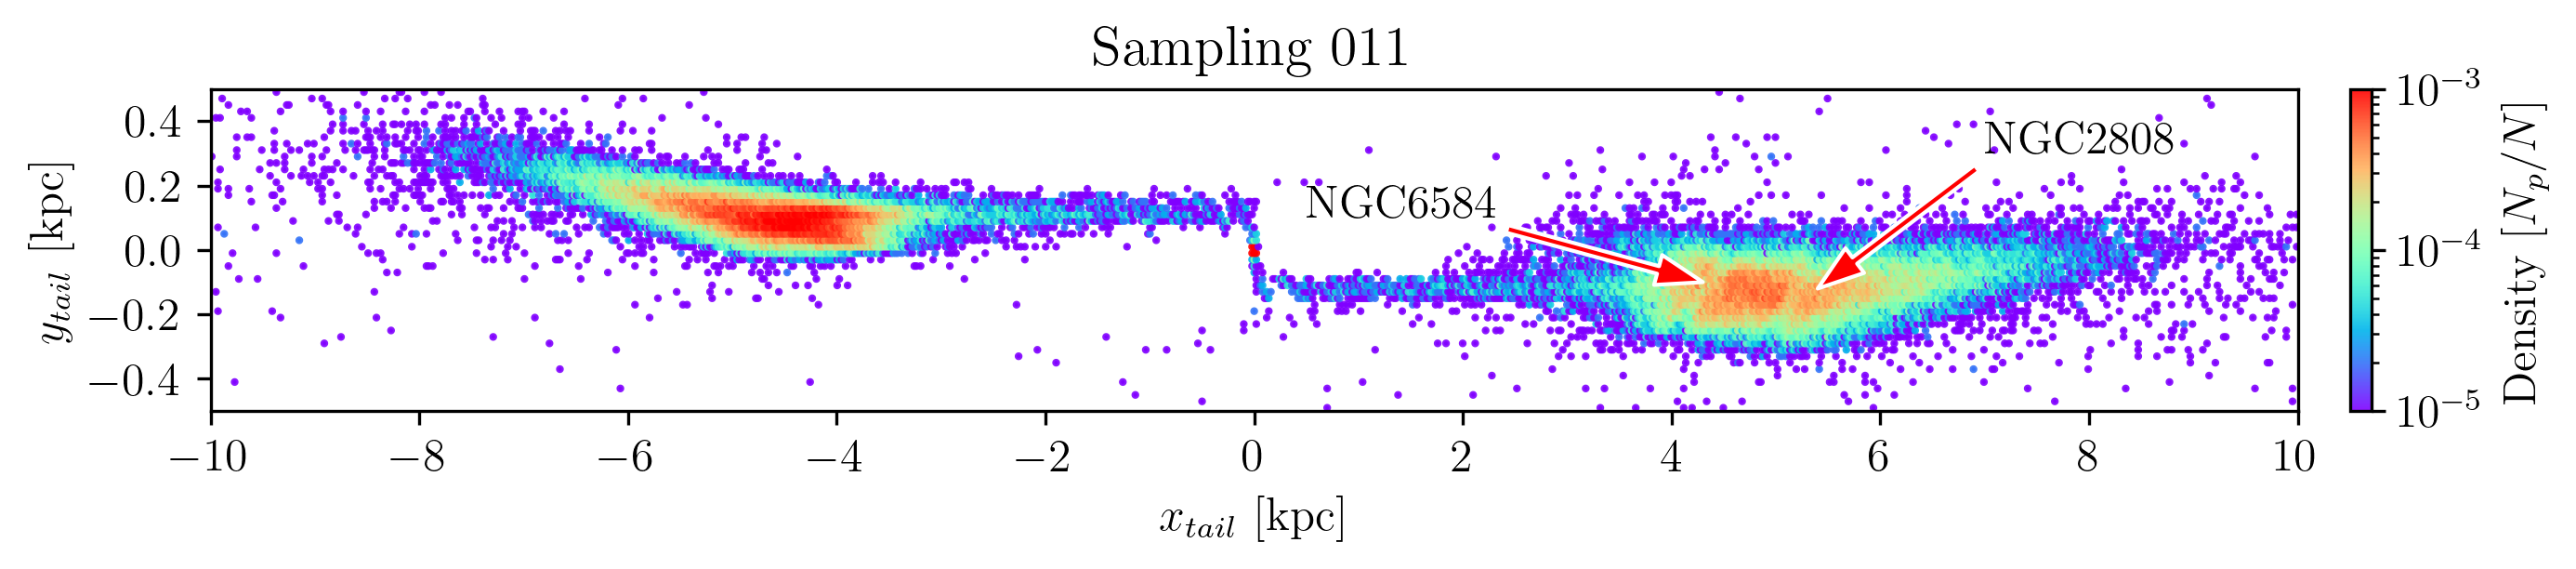
\includegraphics[width=\linewidth]{gallery_of_gaps_monte-carlo-011.png}
      \caption{Gap Gallery}
      \label{fig:TailCoordinates}
    \end{figure*}        


    \begin{figure*}
      \centering
      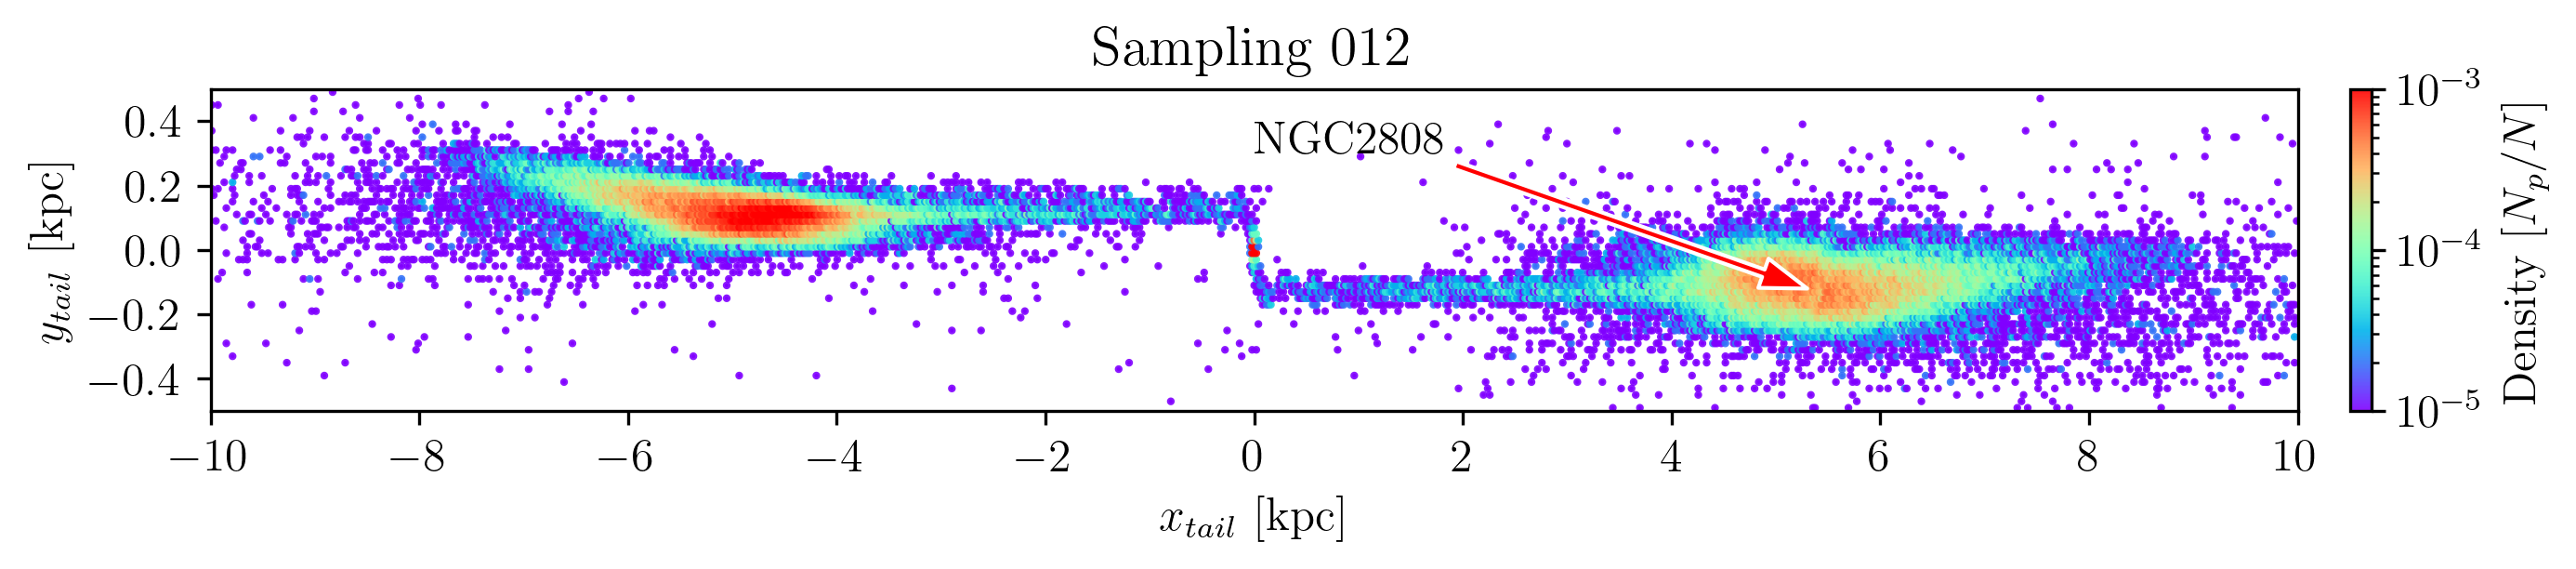
\includegraphics[width=\linewidth]{gallery_of_gaps_monte-carlo-012.png}
      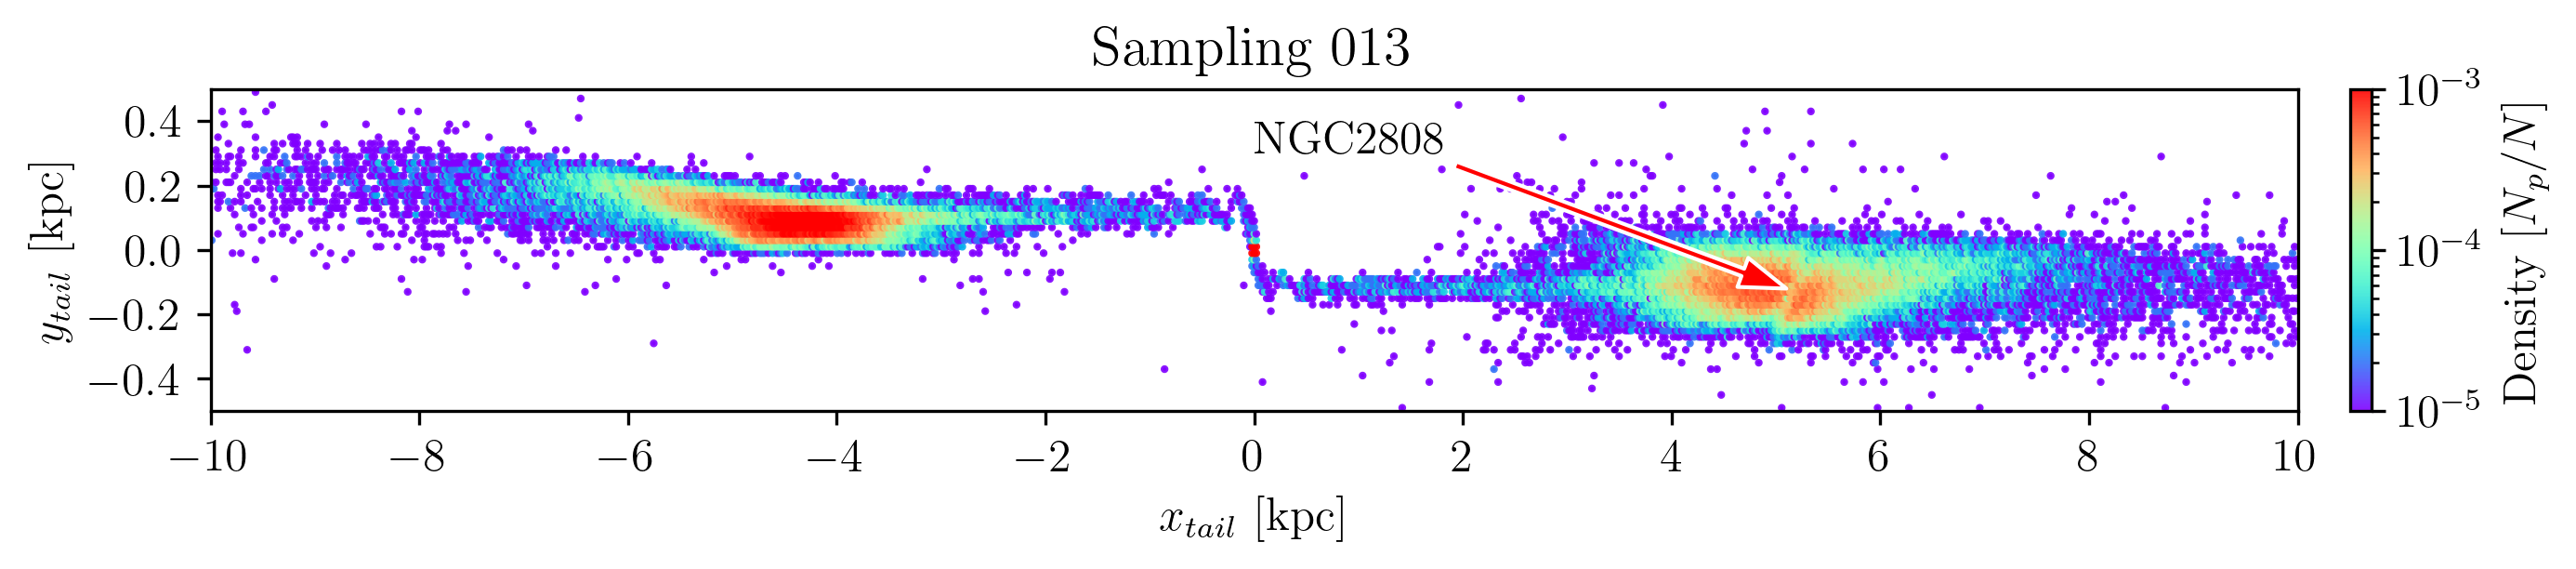
\includegraphics[width=\linewidth]{gallery_of_gaps_monte-carlo-013.png}
      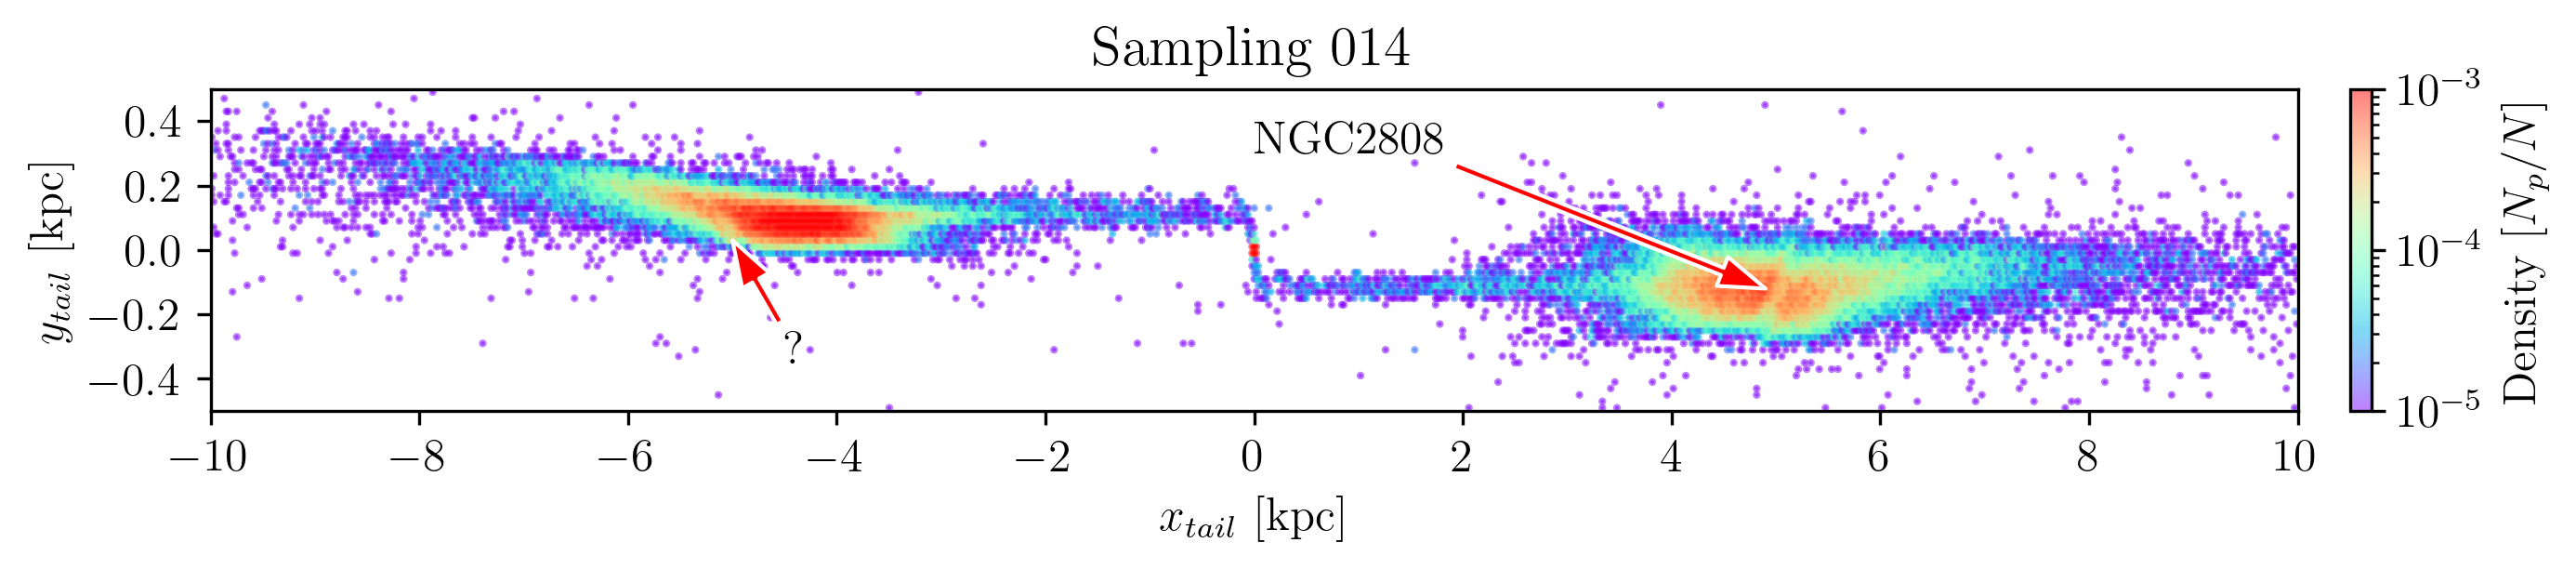
\includegraphics[width=\linewidth]{gallery_of_gaps_monte-carlo-014.png}      
      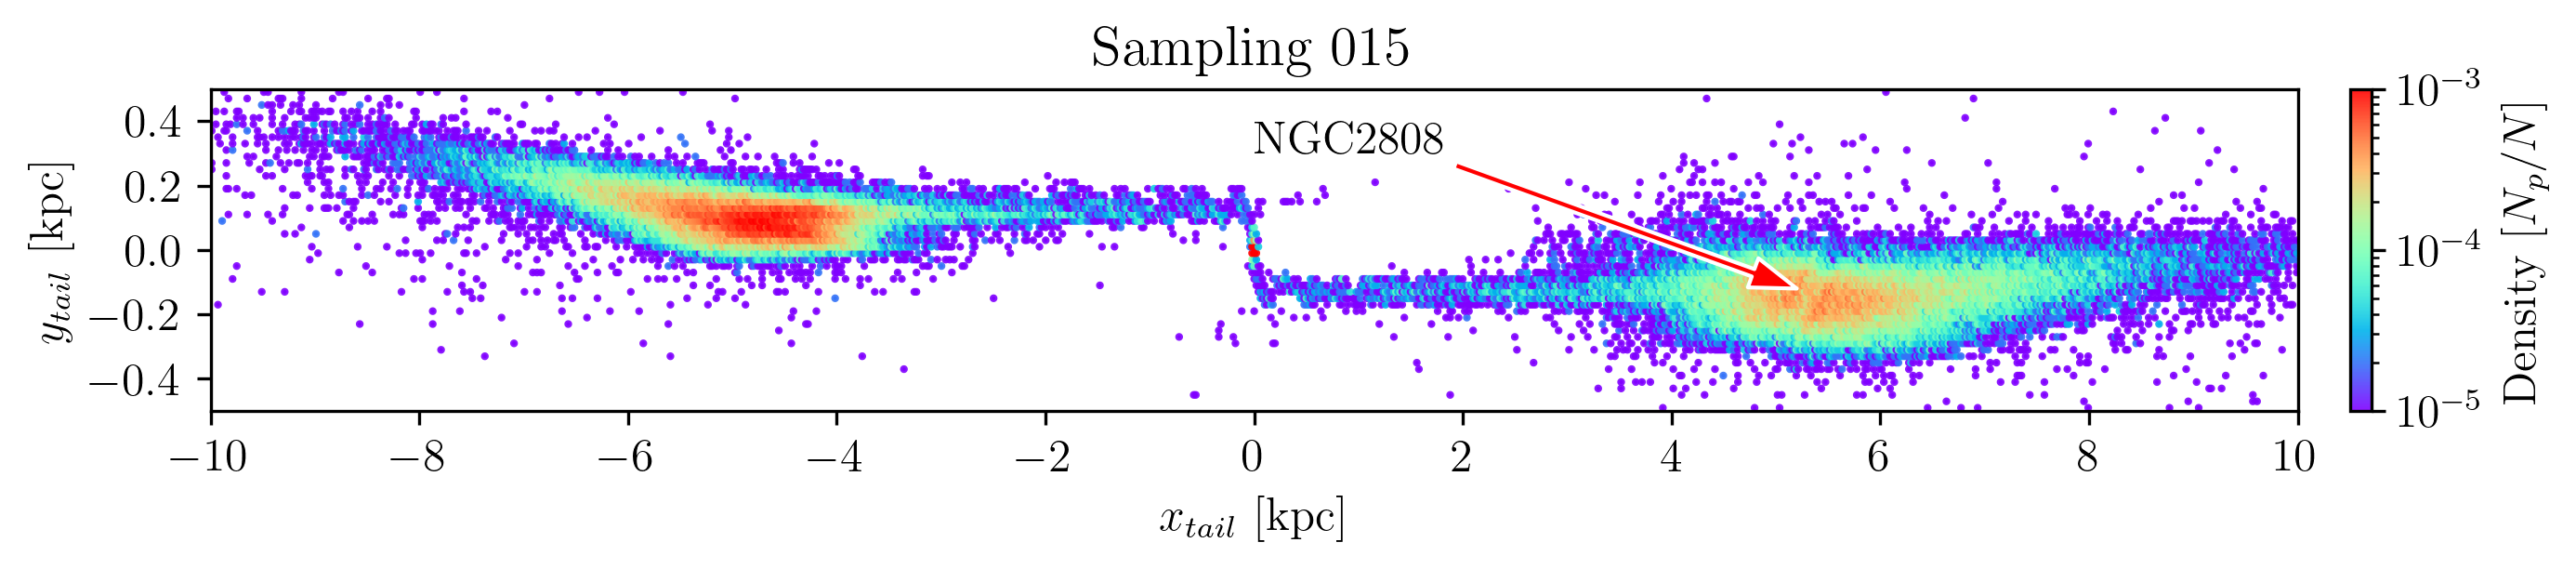
\includegraphics[width=\linewidth]{gallery_of_gaps_monte-carlo-015.png}
      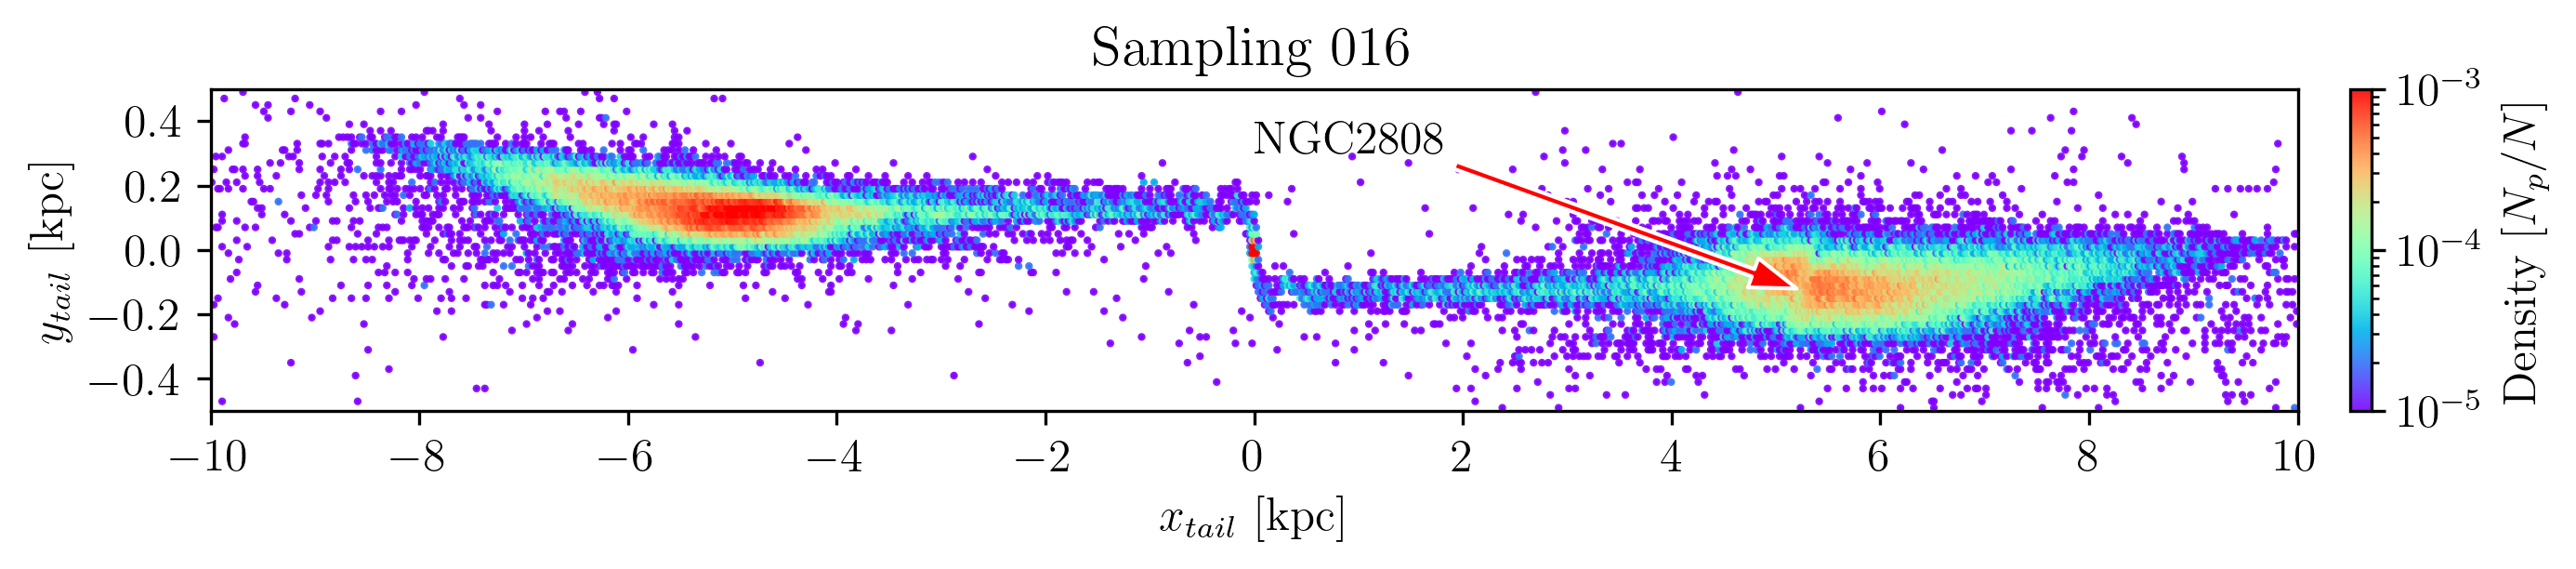
\includegraphics[width=\linewidth]{gallery_of_gaps_monte-carlo-016.png}
      \caption{Gap Gallery}
      \label{fig:TailCoordinates}
    \end{figure*}        

    \begin{figure*}
      \centering
      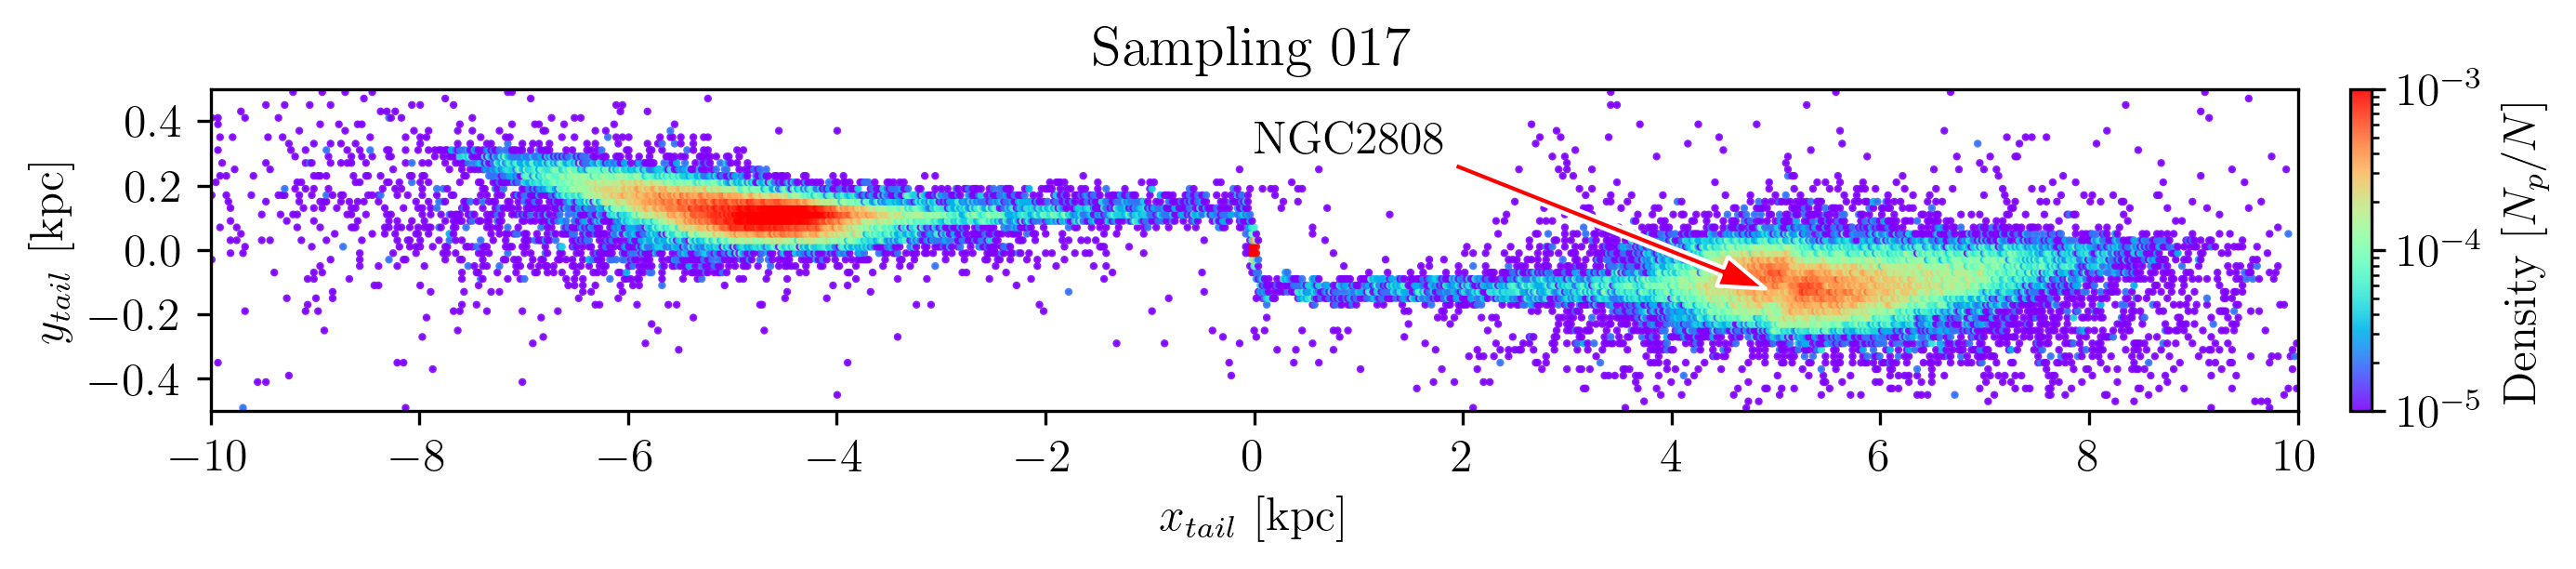
\includegraphics[width=\linewidth]{gallery_of_gaps_monte-carlo-017.png}
      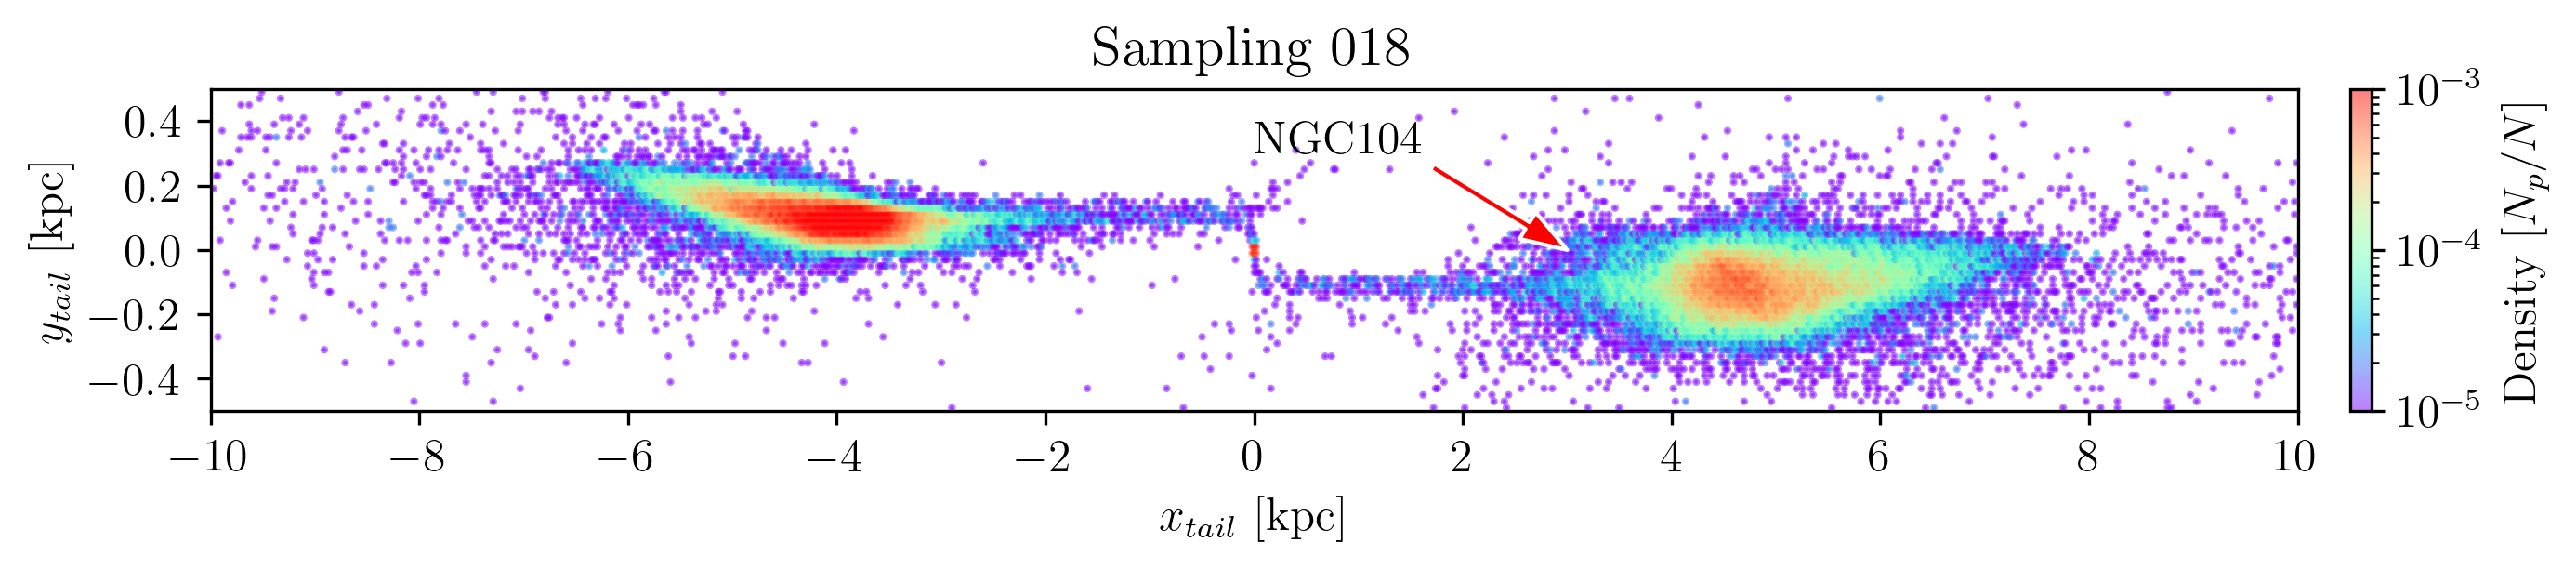
\includegraphics[width=\linewidth]{gallery_of_gaps_monte-carlo-018.png}
      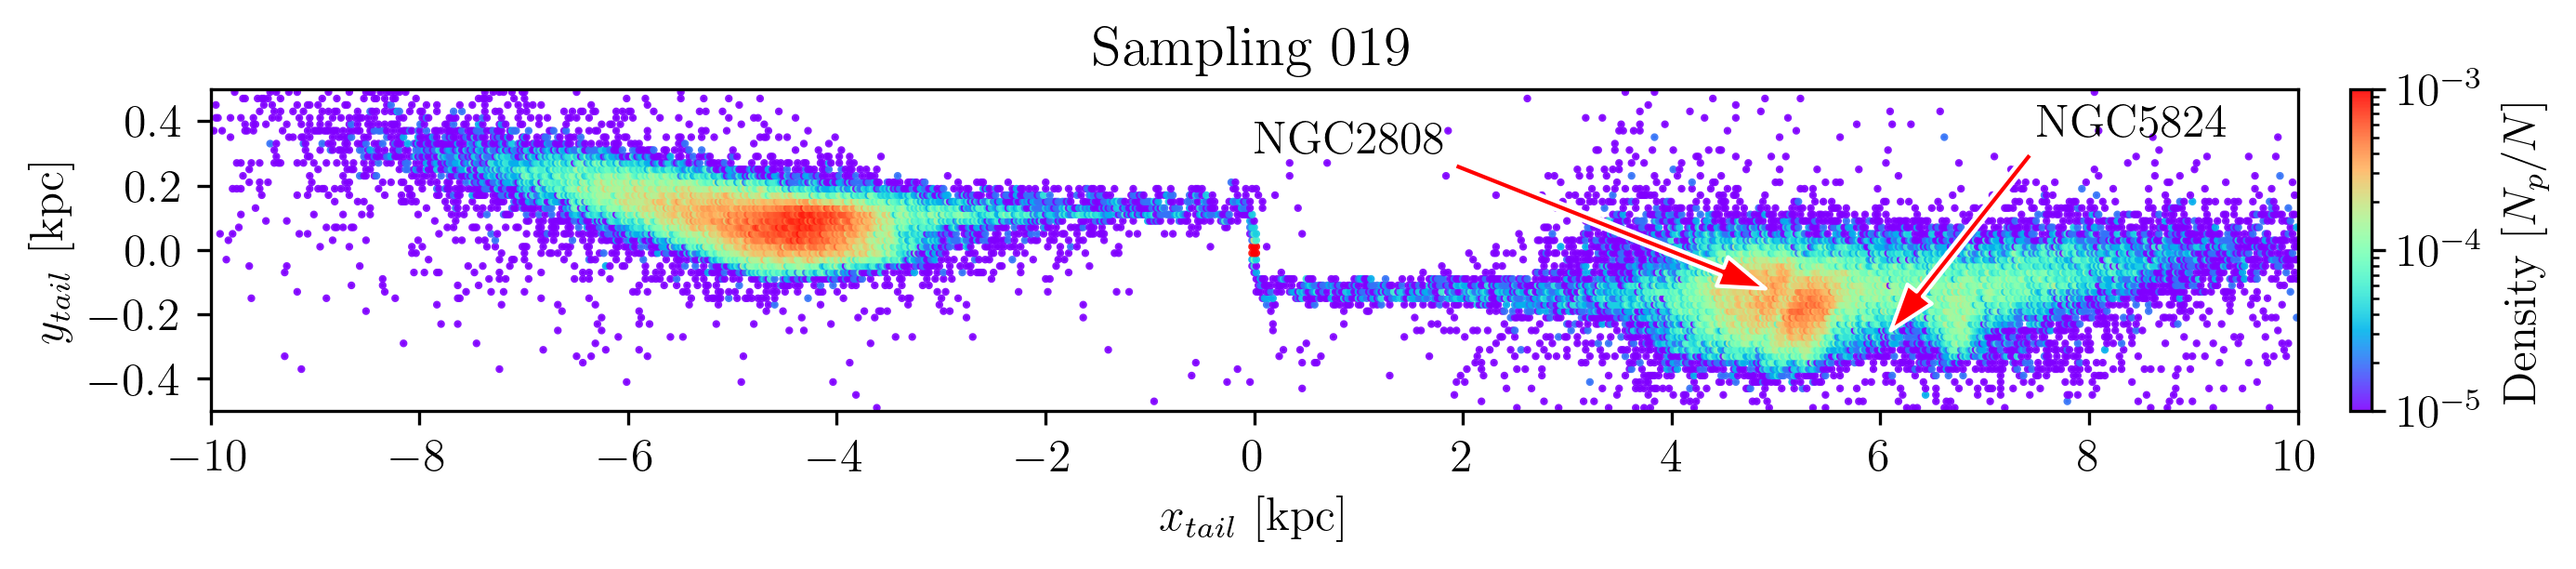
\includegraphics[width=\linewidth]{gallery_of_gaps_monte-carlo-019.png}      
      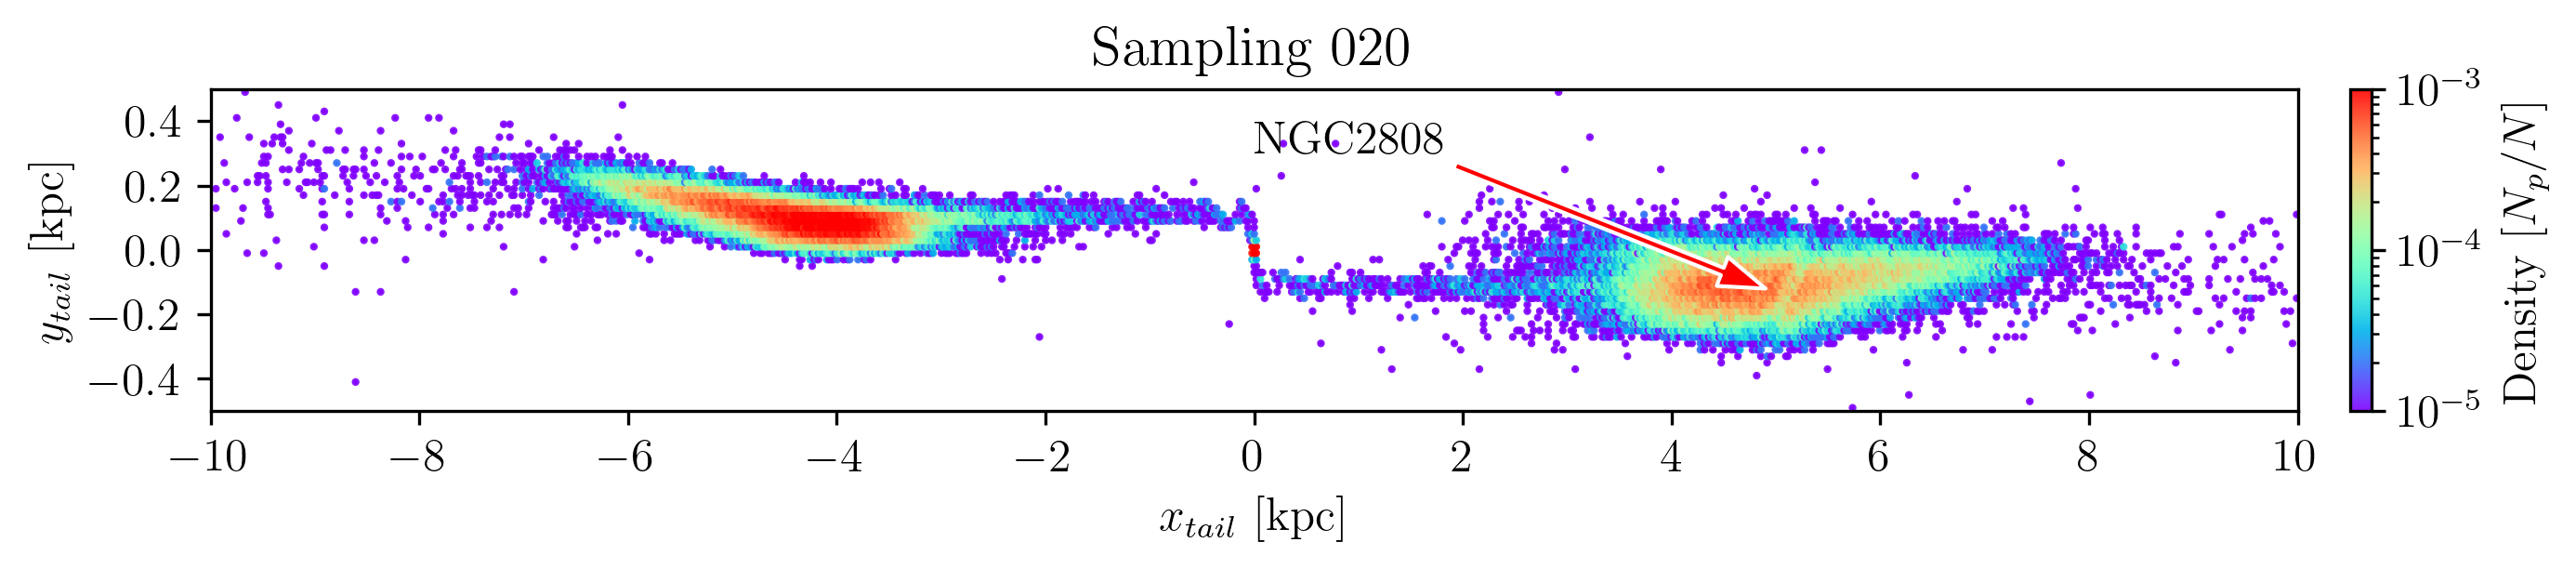
\includegraphics[width=\linewidth]{gallery_of_gaps_monte-carlo-020.png}
      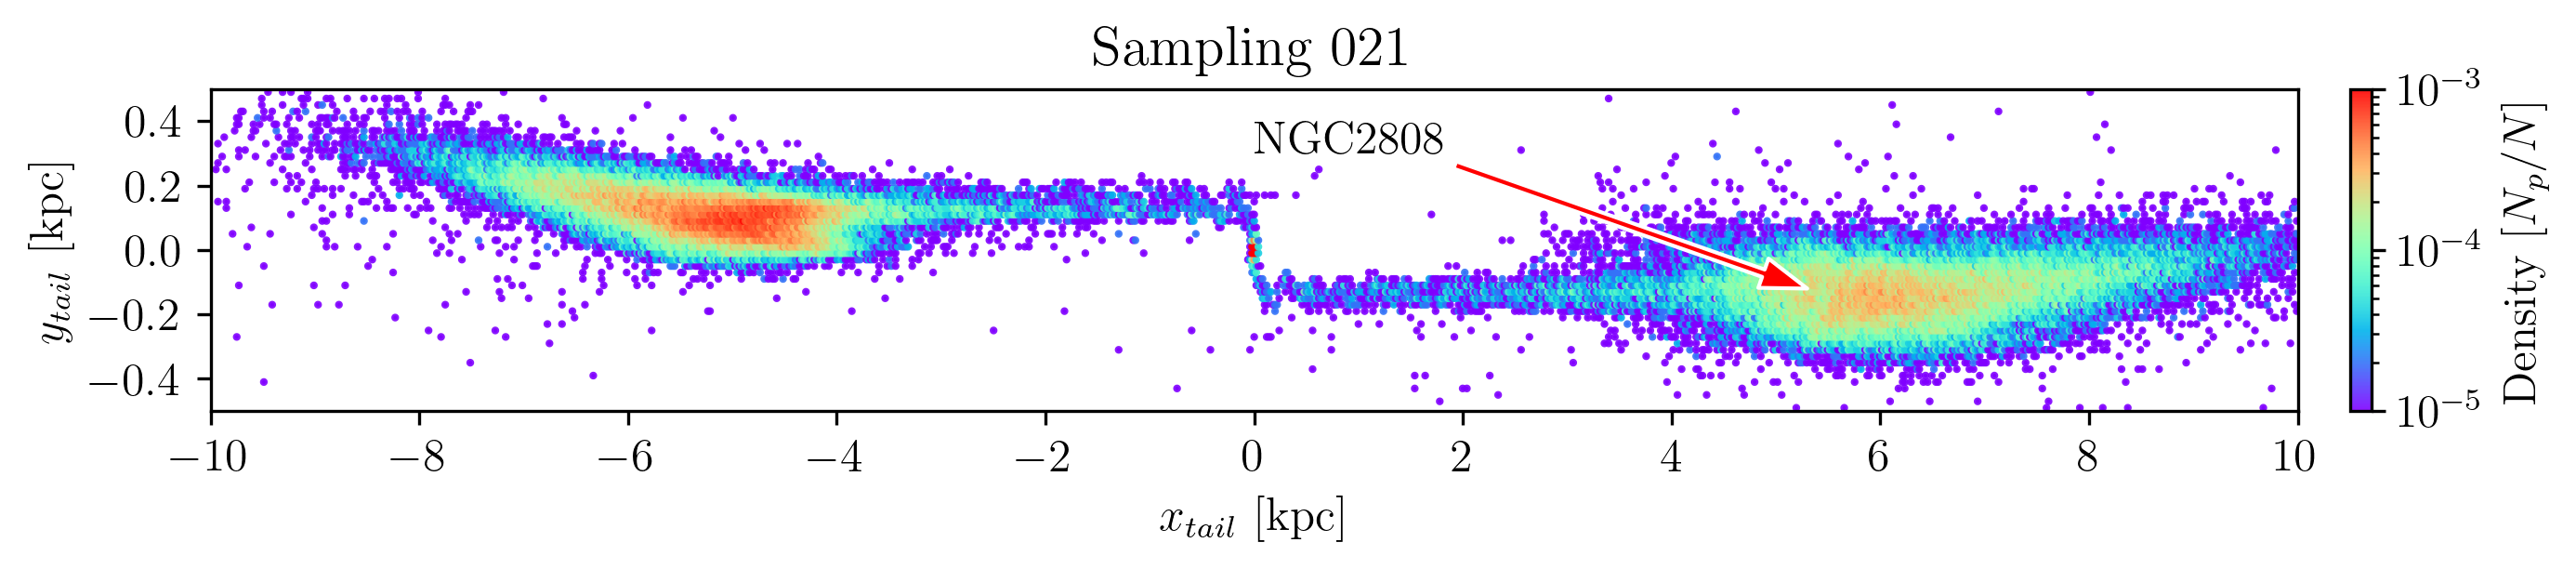
\includegraphics[width=\linewidth]{gallery_of_gaps_monte-carlo-021.png}
      \caption{Gap Gallery}
      \label{fig:TailCoordinates}
    \end{figure*}        

    \begin{figure*}
      \centering
      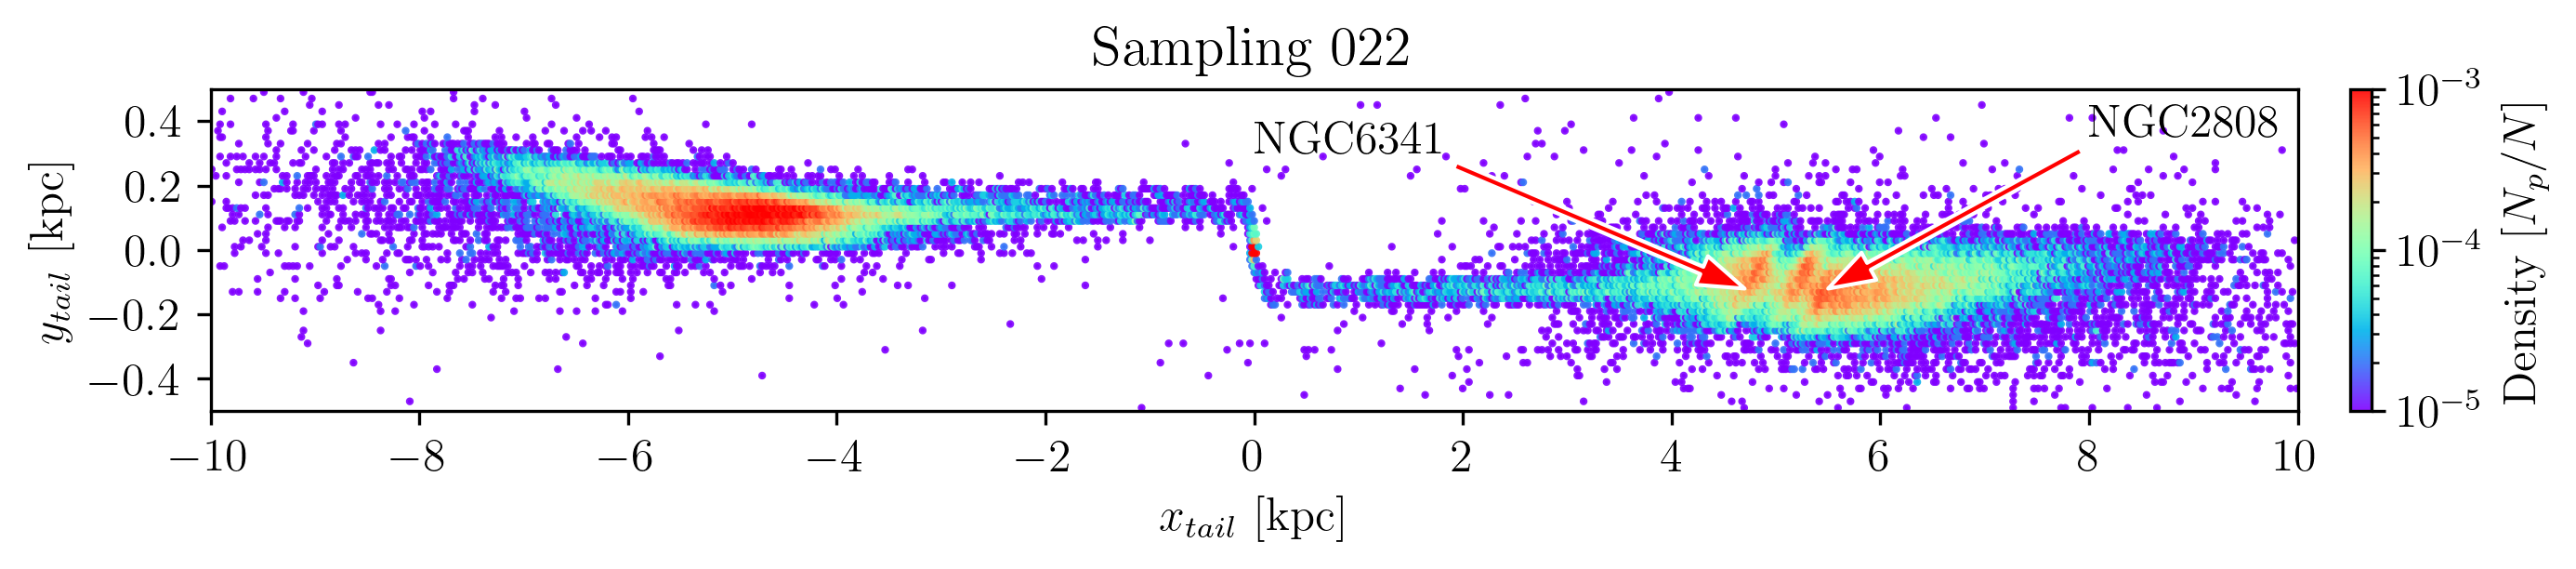
\includegraphics[width=\linewidth]{gallery_of_gaps_monte-carlo-022.png}
      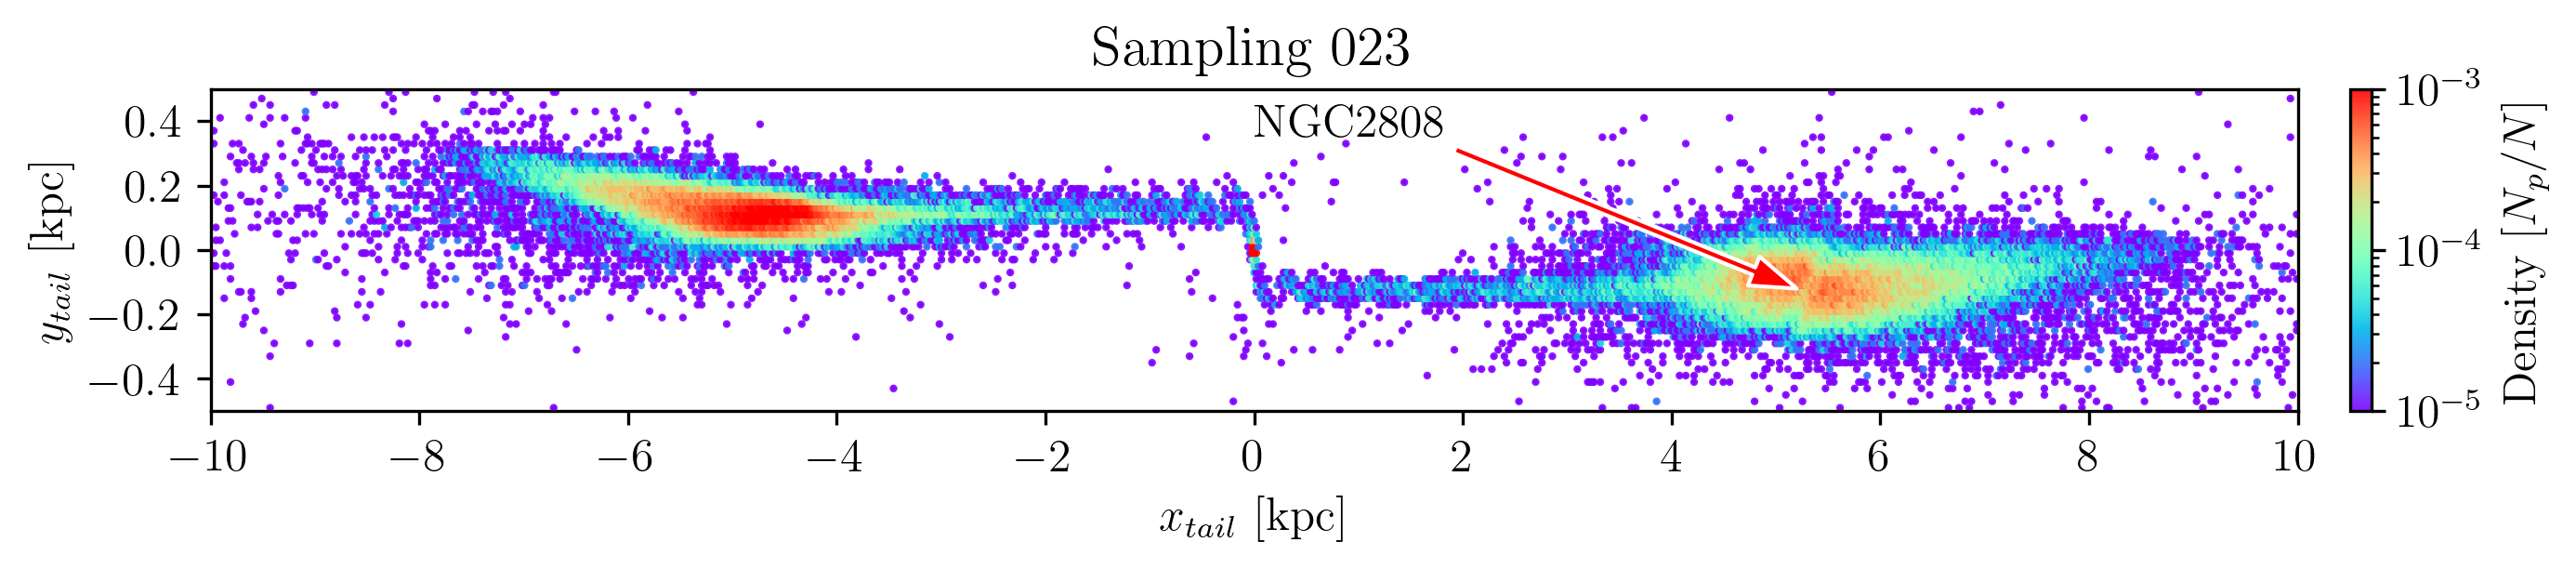
\includegraphics[width=\linewidth]{gallery_of_gaps_monte-carlo-023.png}
      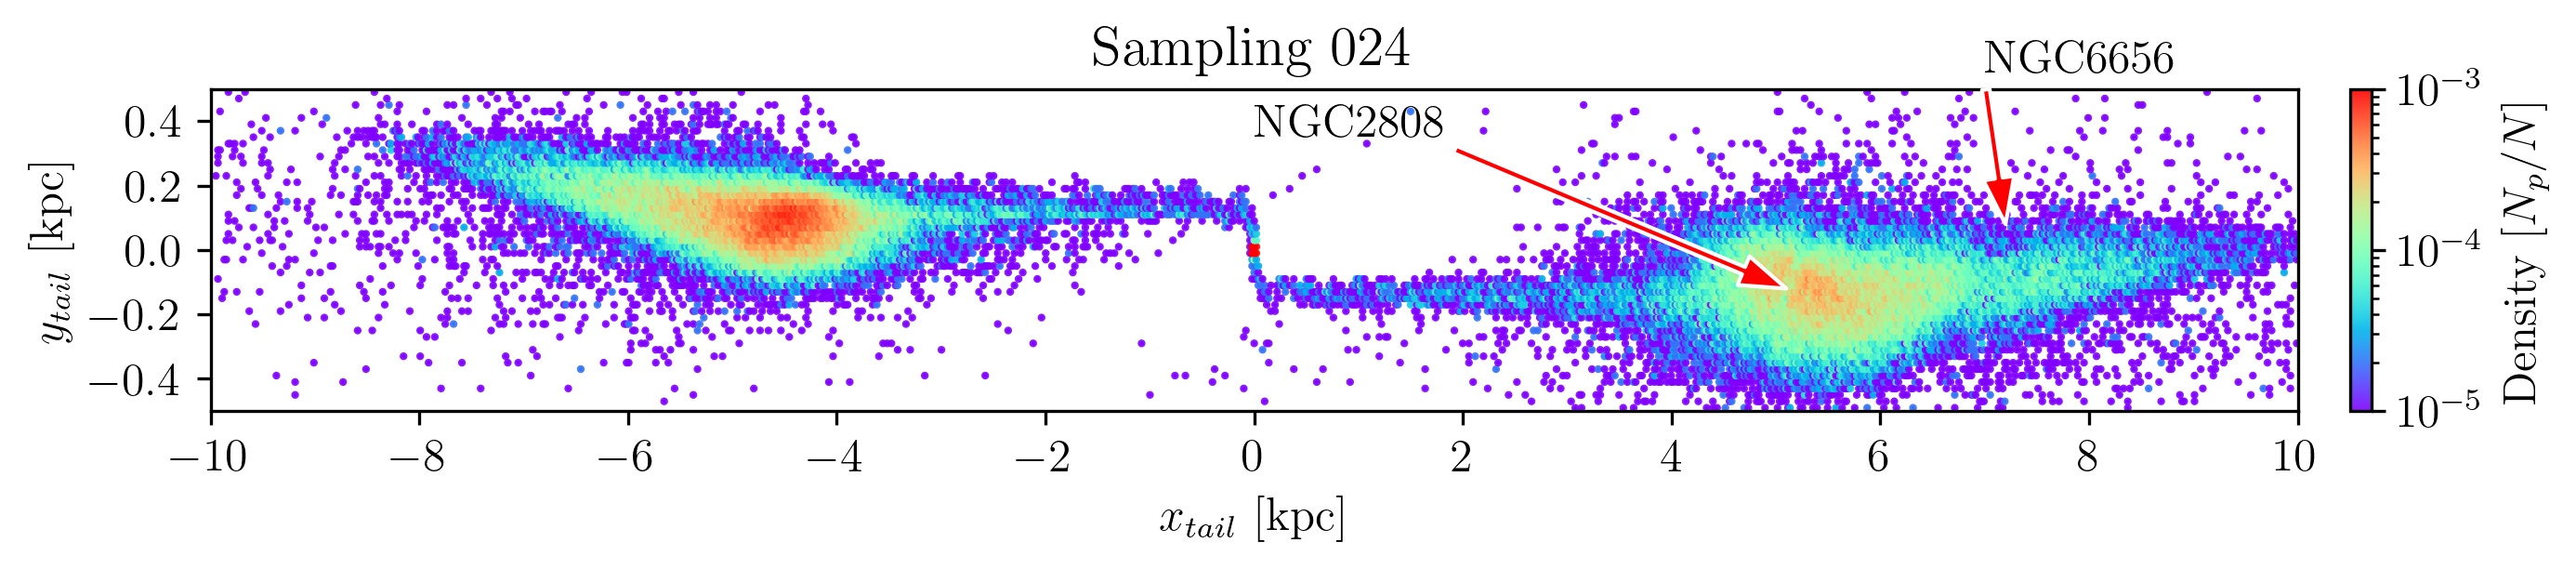
\includegraphics[width=\linewidth]{gallery_of_gaps_monte-carlo-024.png}   
      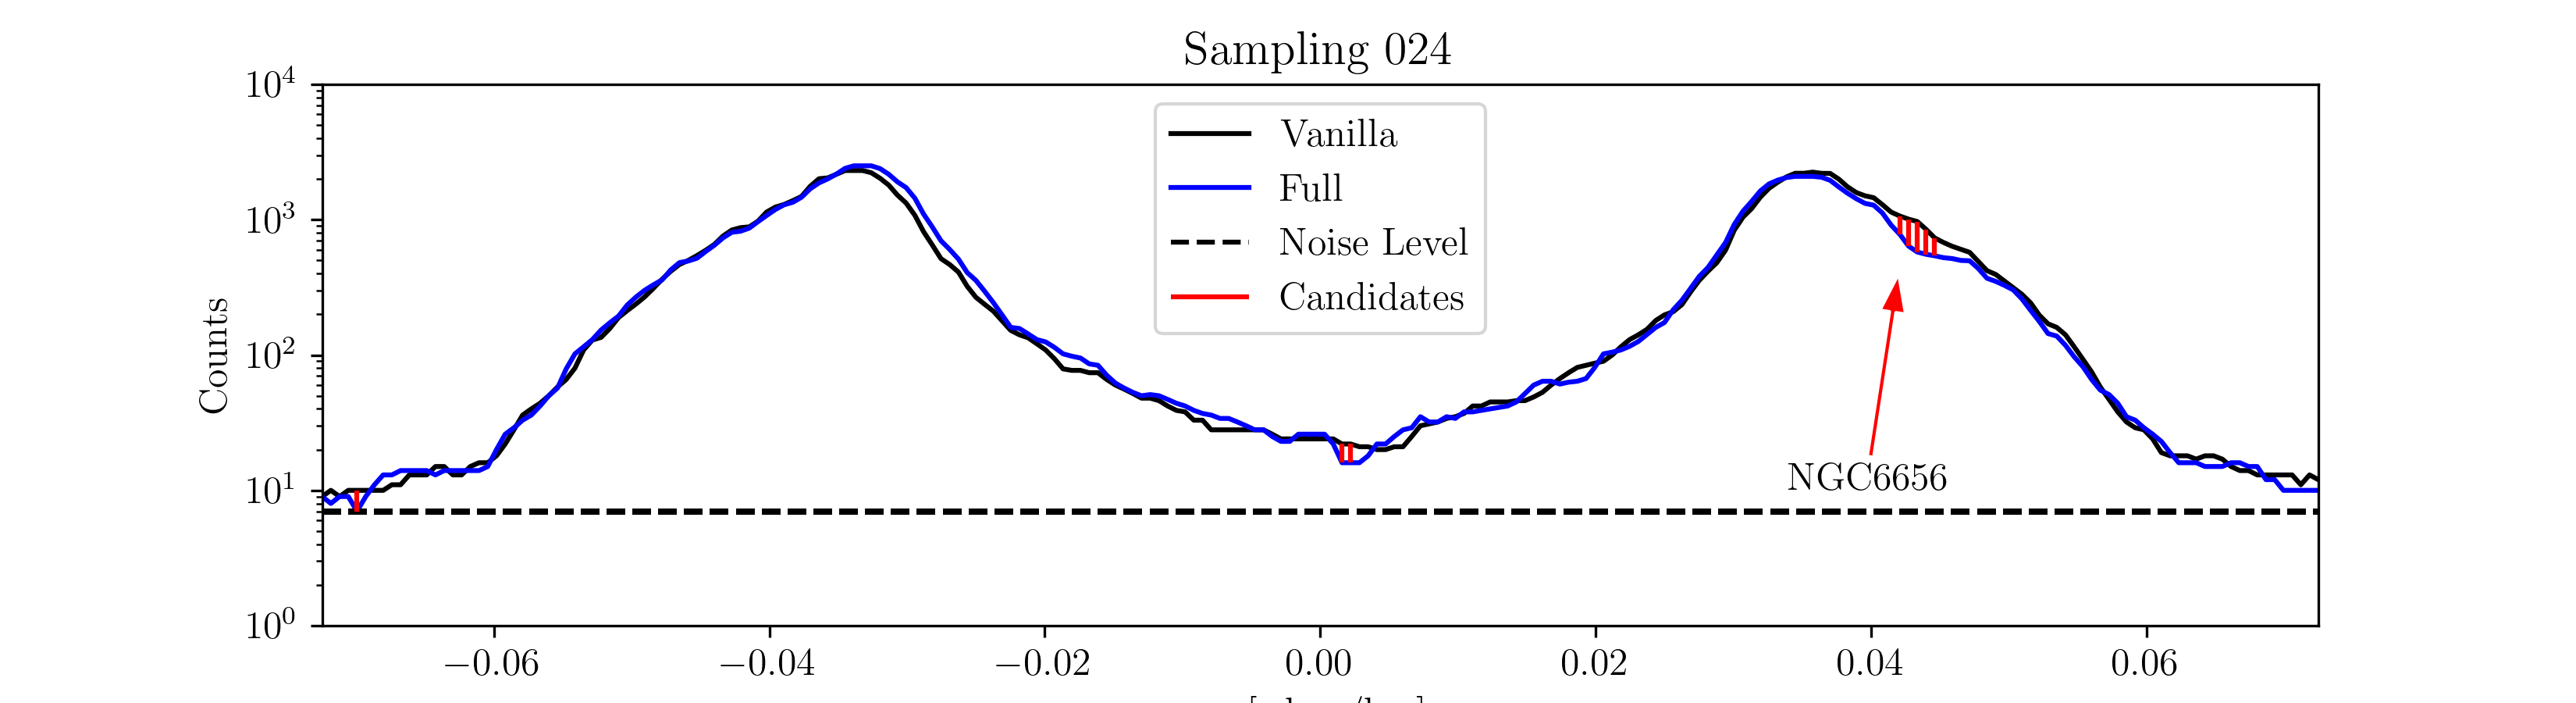
\includegraphics[width=\linewidth]{tau-profile-monte-carlo-024.png}
      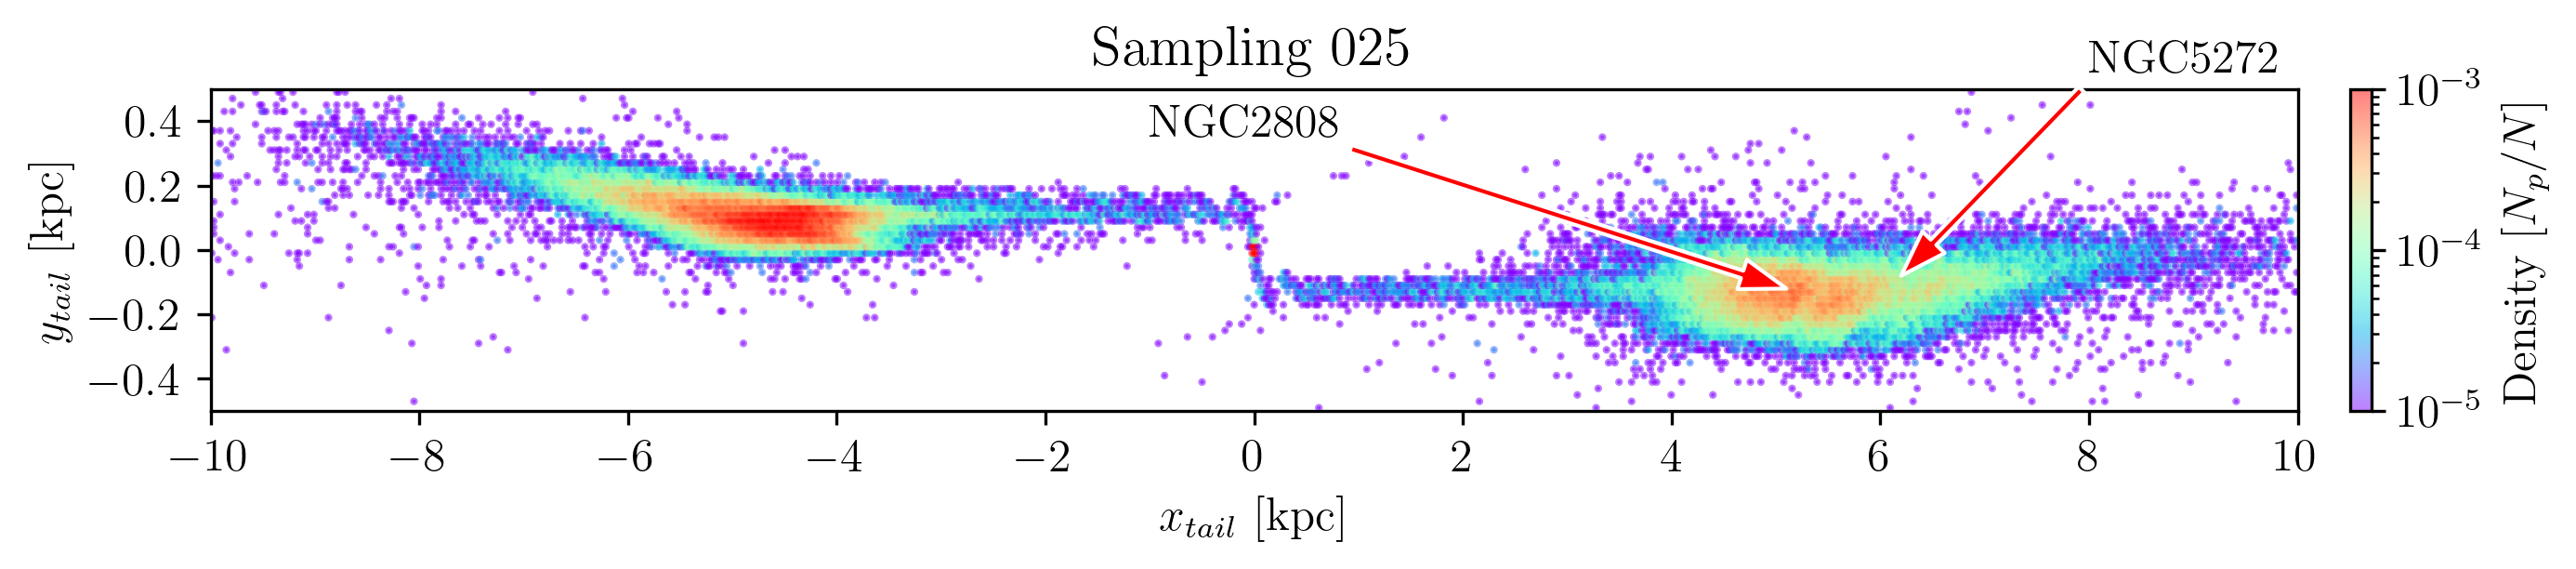
\includegraphics[width=\linewidth]{gallery_of_gaps_monte-carlo-025.png}
      \caption{Gap Gallery}
      \label{fig:TailCoordinates}
    \end{figure*}        

    \begin{figure*}
      \centering
      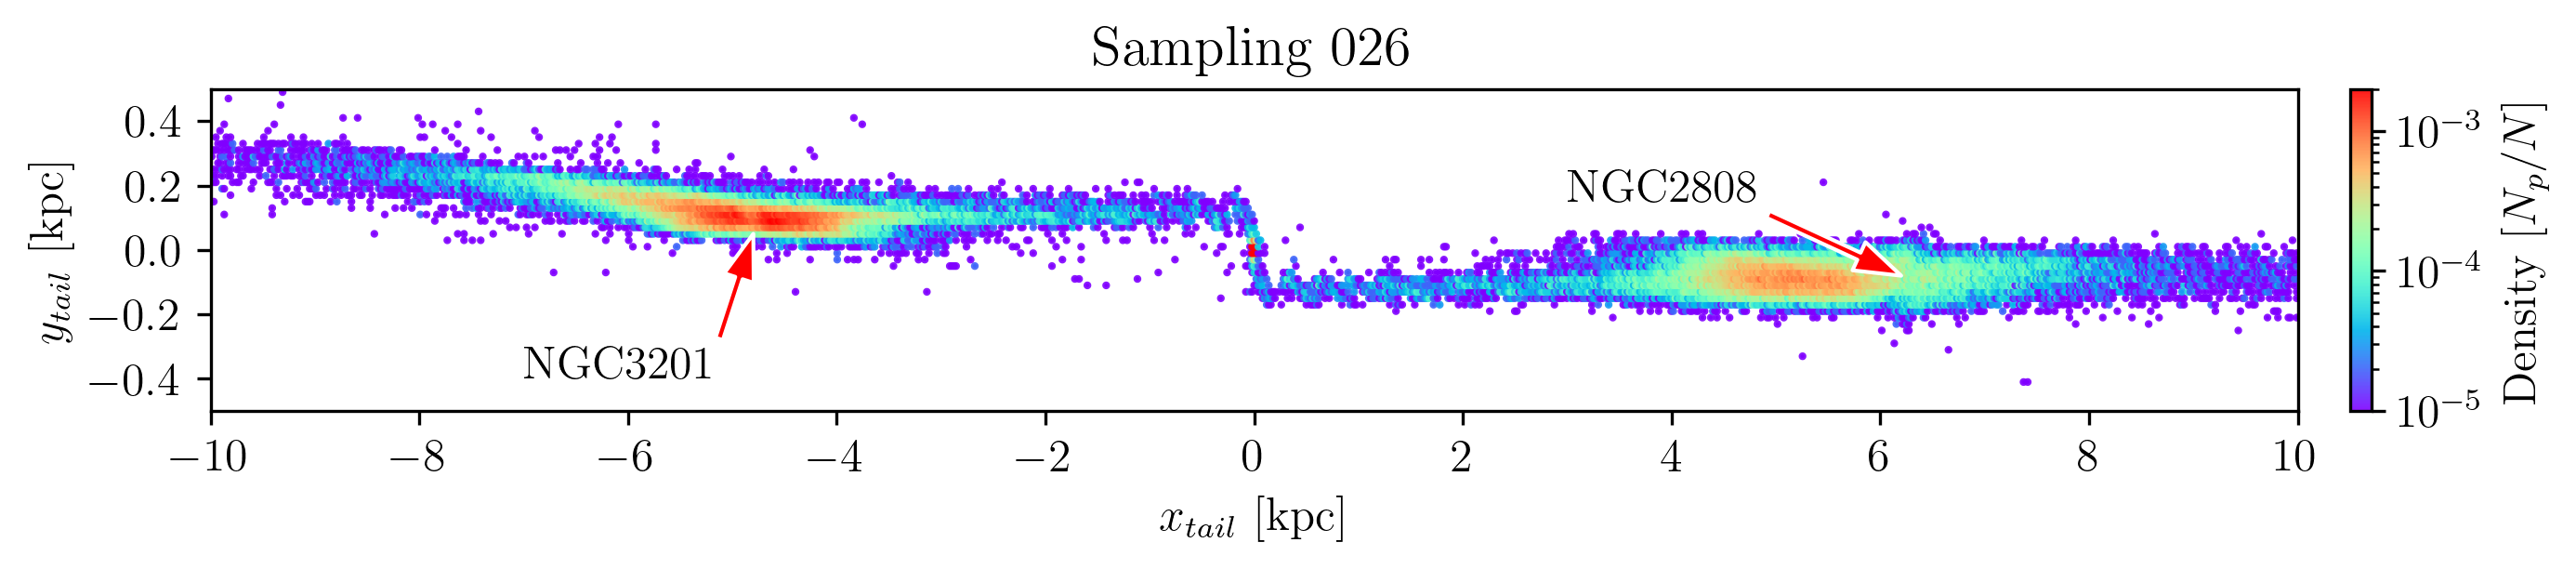
\includegraphics[width=\linewidth]{gallery_of_gaps_monte-carlo-026.png}
      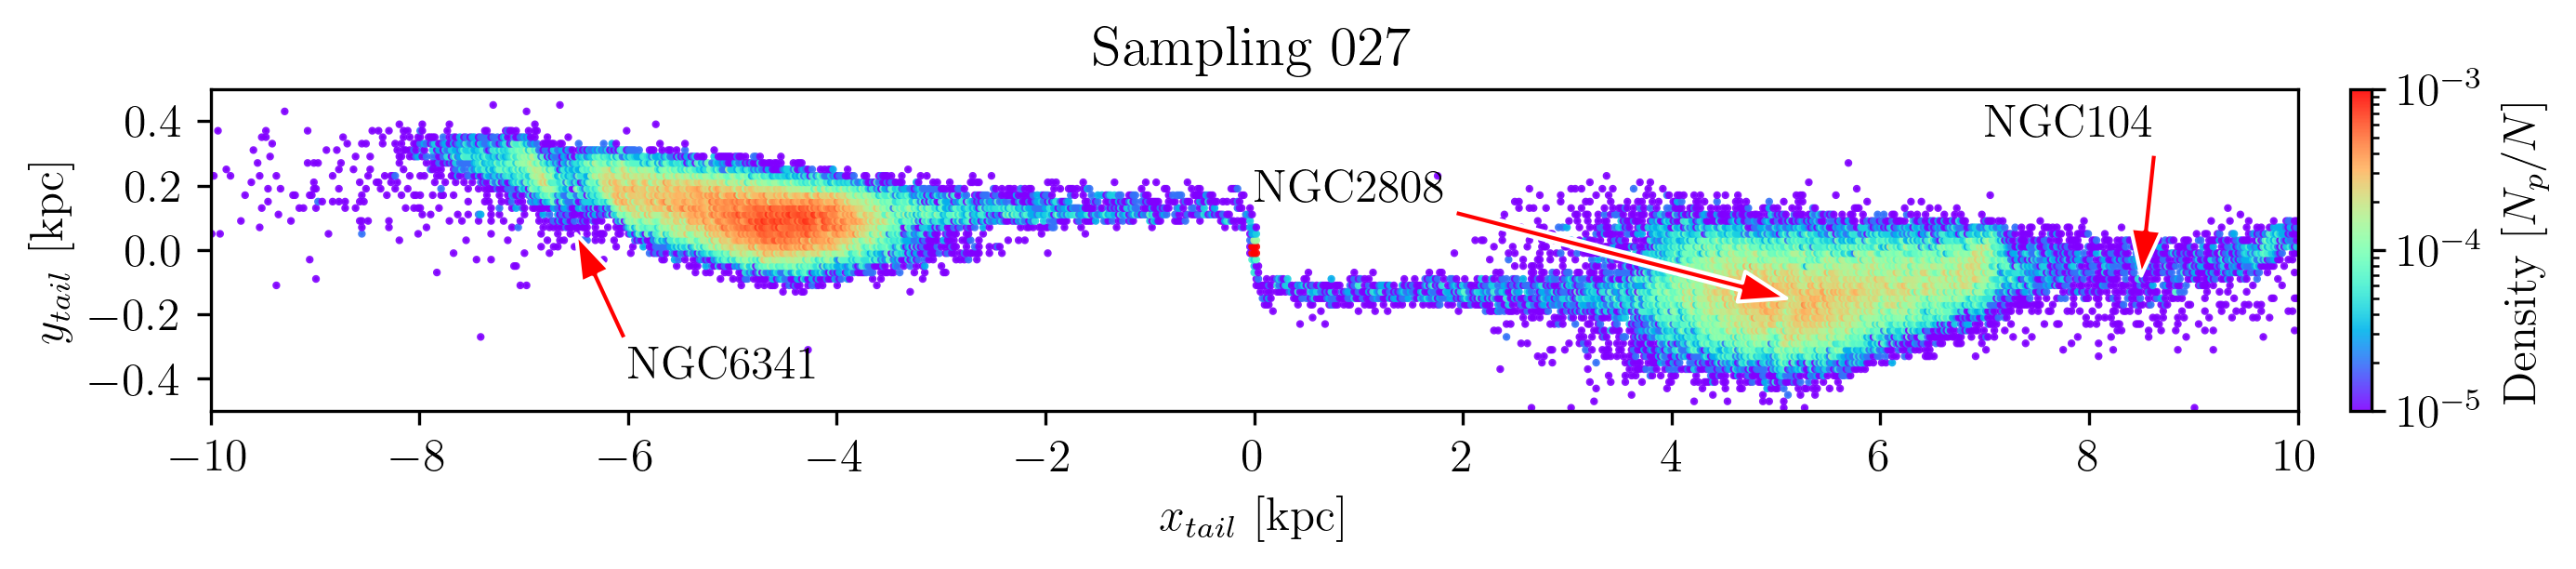
\includegraphics[width=\linewidth]{gallery_of_gaps_monte-carlo-027.png}
      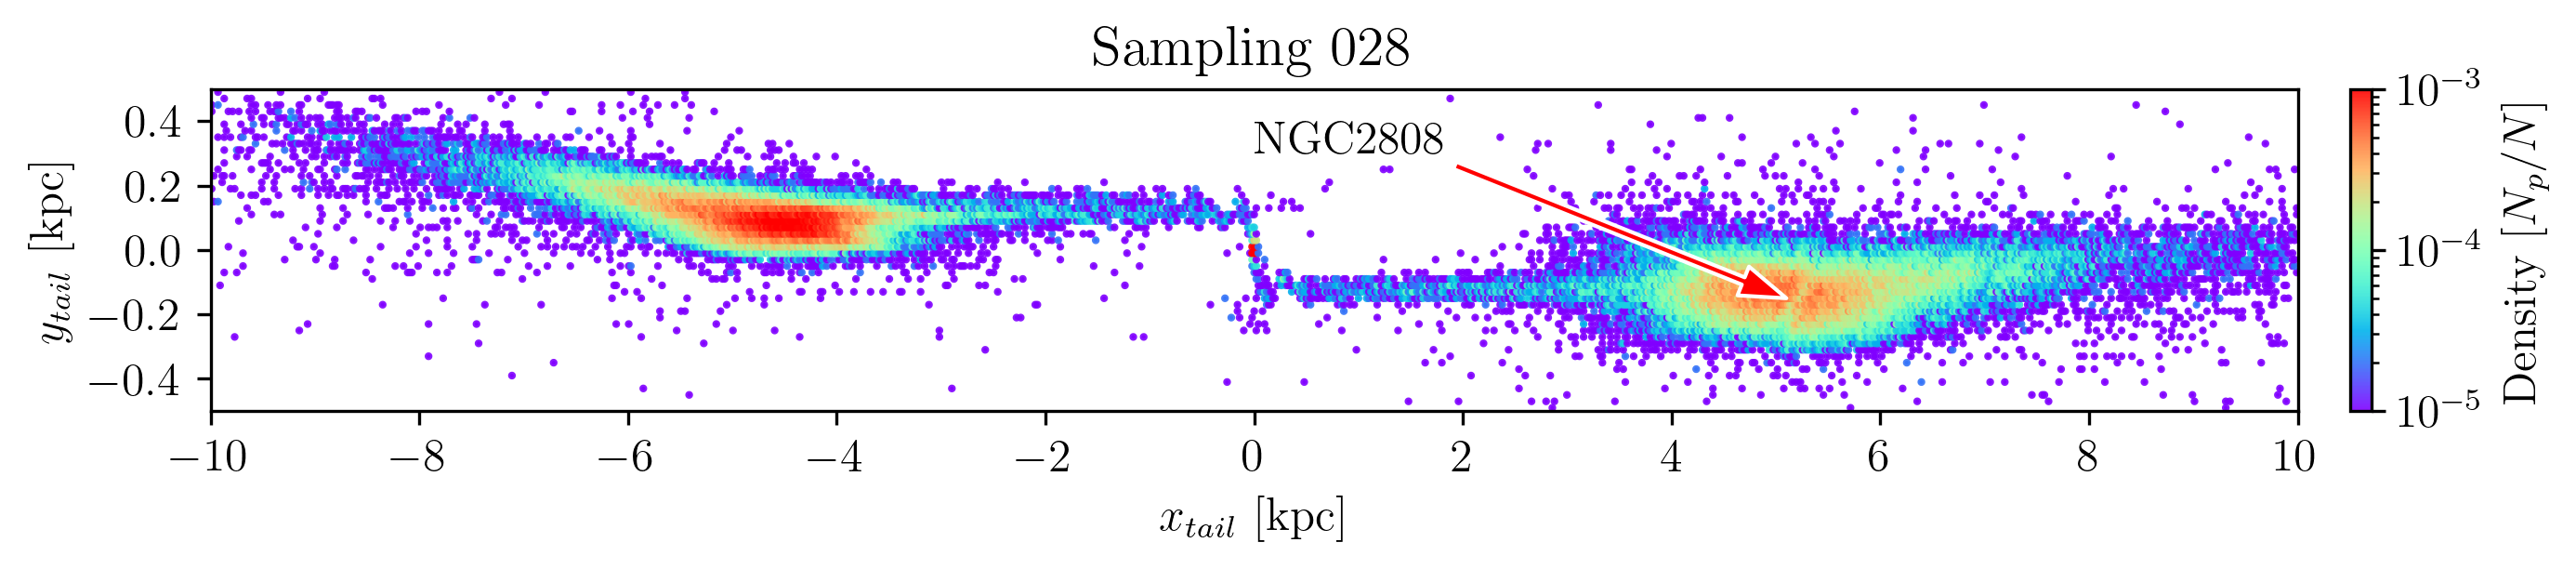
\includegraphics[width=\linewidth]{gallery_of_gaps_monte-carlo-028.png}
      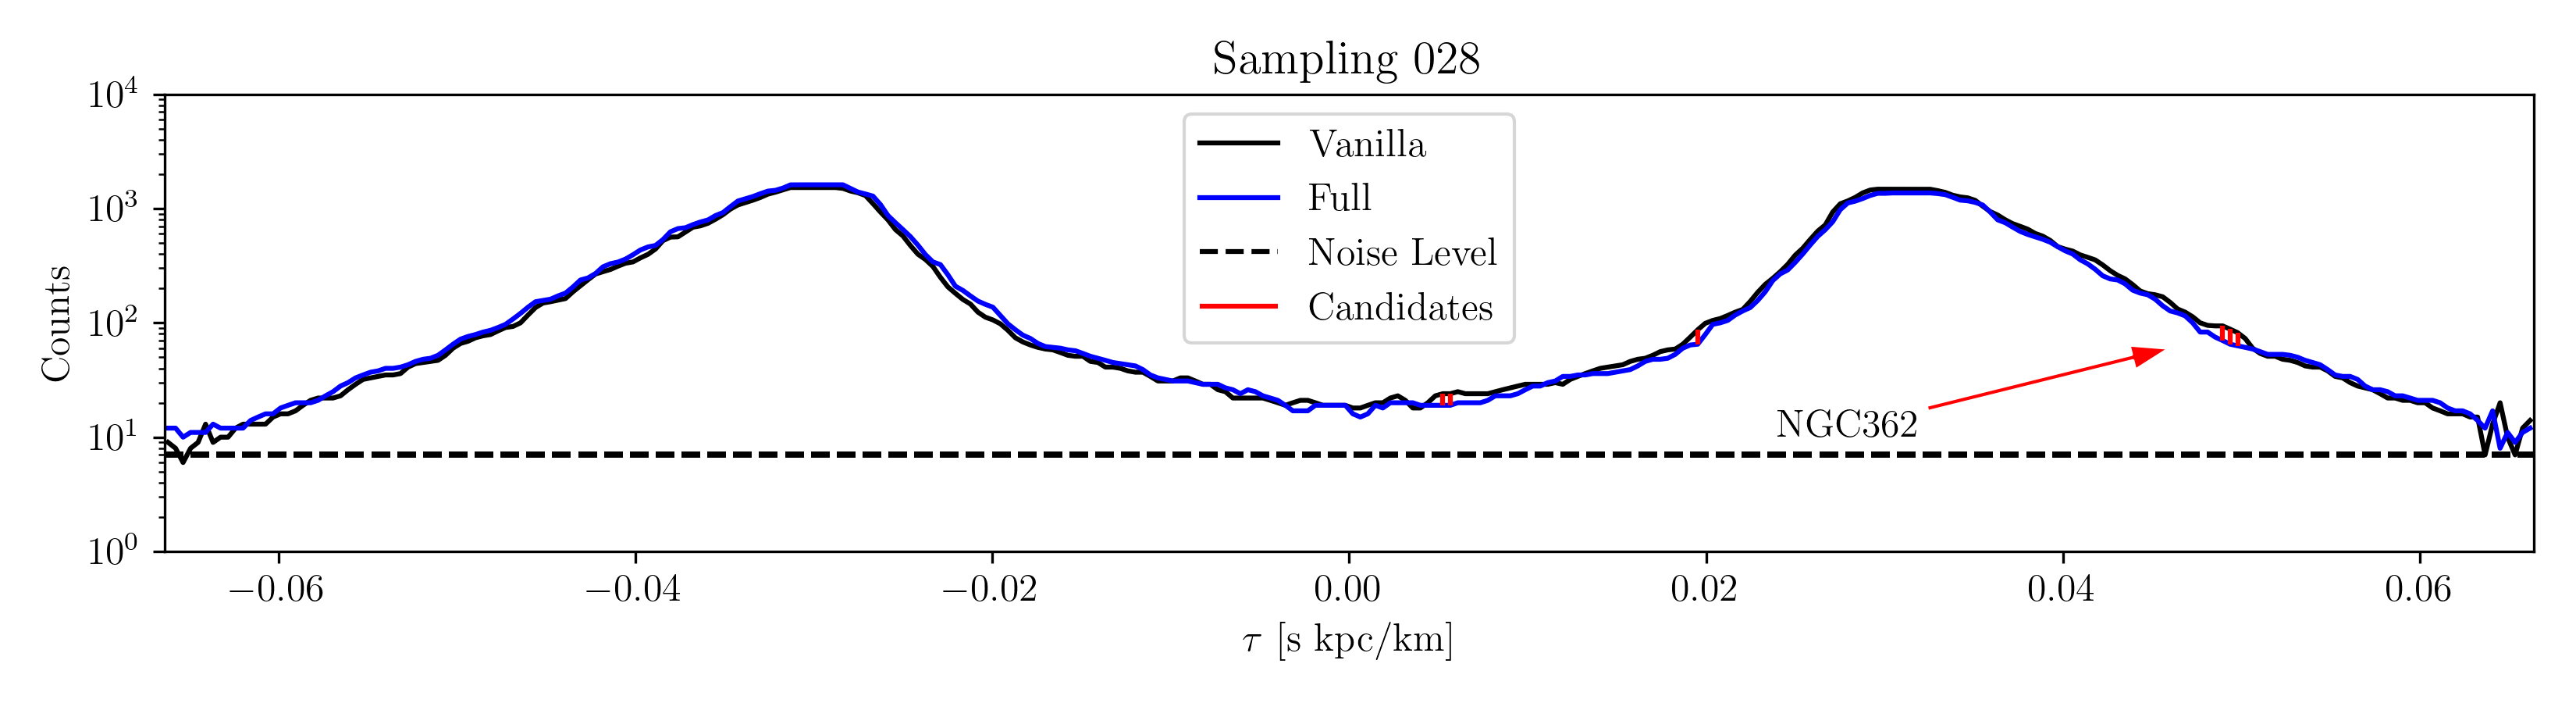
\includegraphics[width=\linewidth]{tau-profile-monte-carlo-028.png}
      \caption{Gap Gallery}
      \label{fig:TailCoordinates}
    \end{figure*}        

    \begin{figure*}
      \centering      
      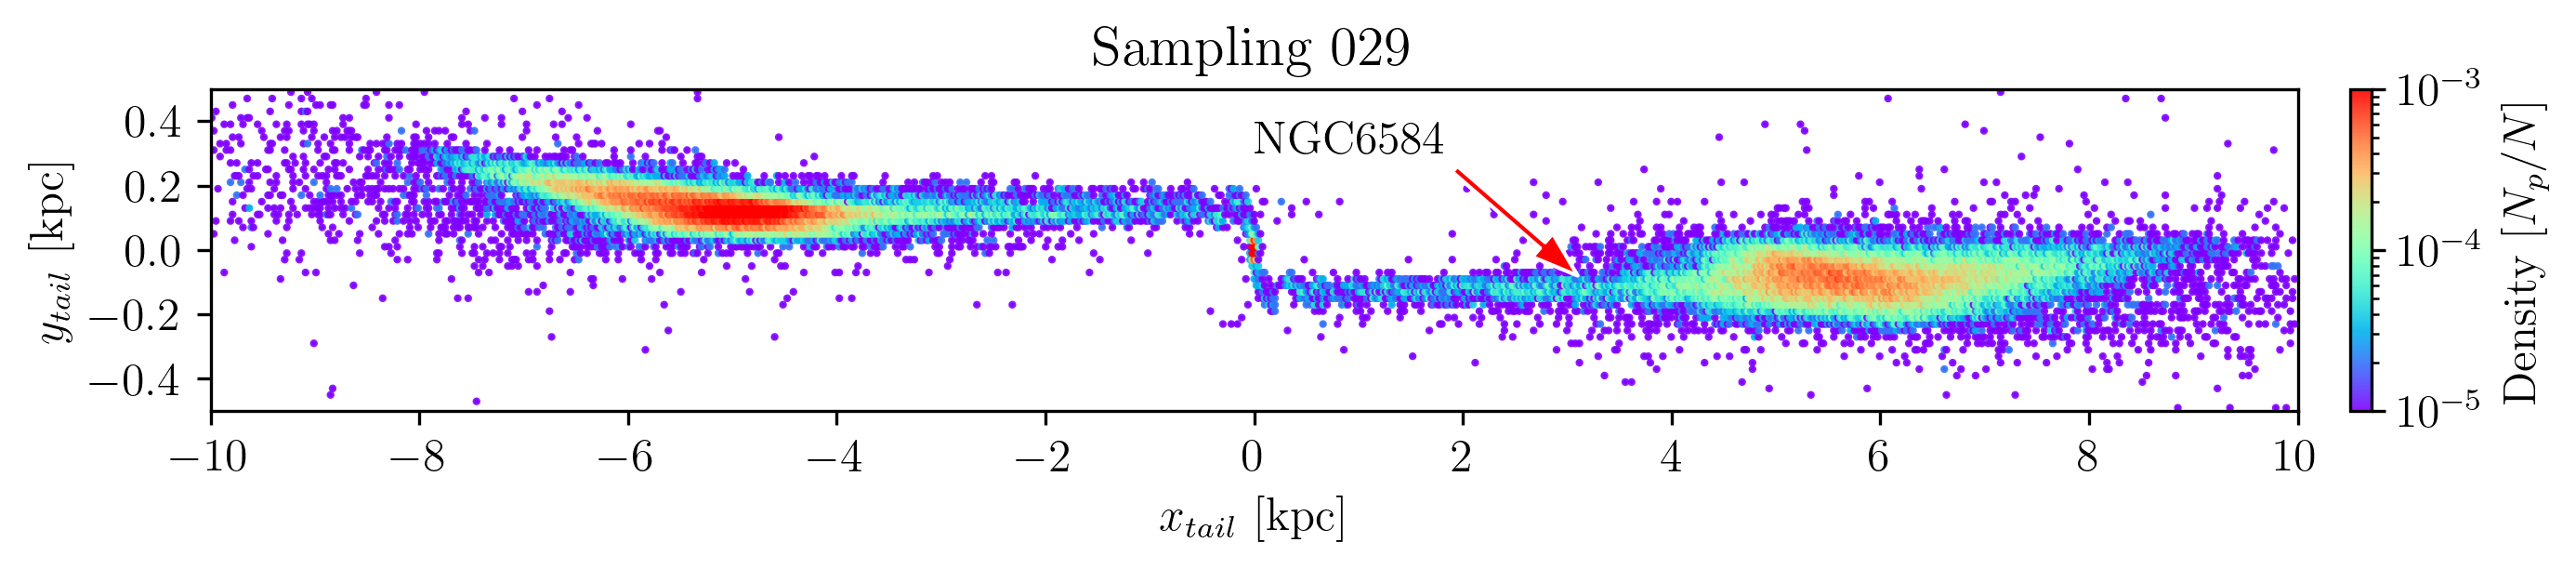
\includegraphics[width=\linewidth]{gallery_of_gaps_monte-carlo-029.png}    
      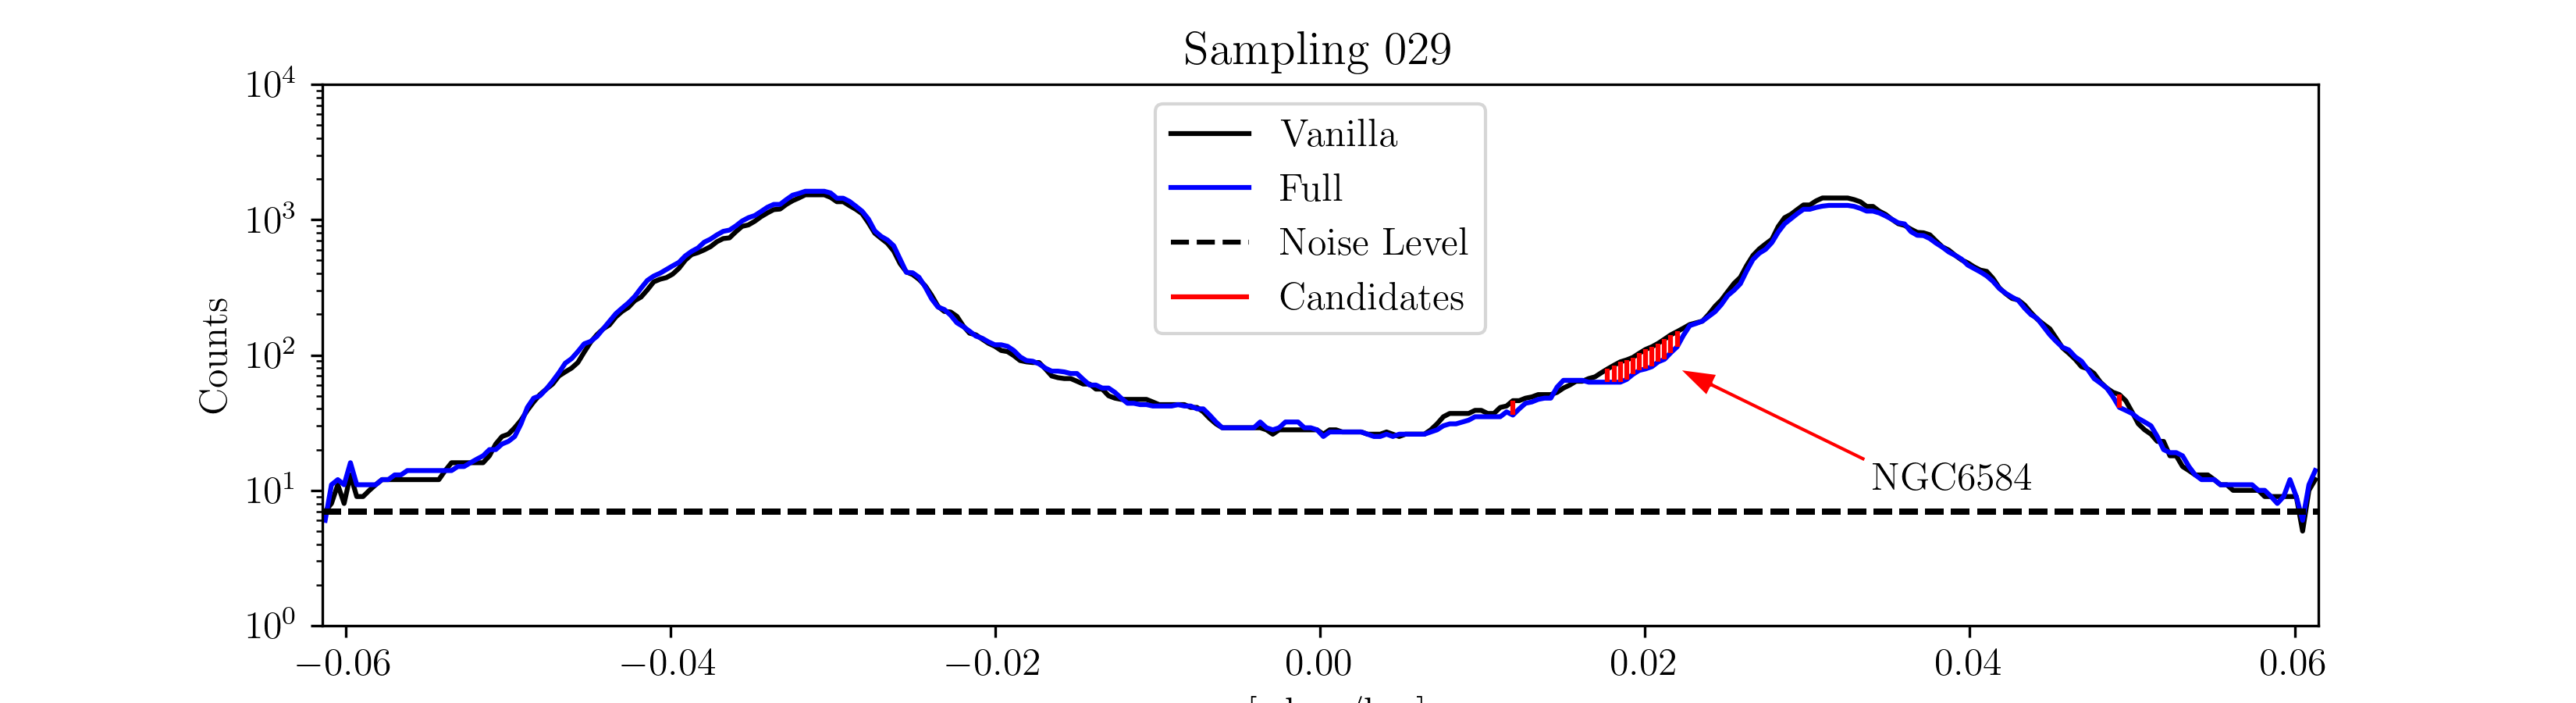
\includegraphics[width=\linewidth]{tau-profile-monte-carlo-029.png}  
      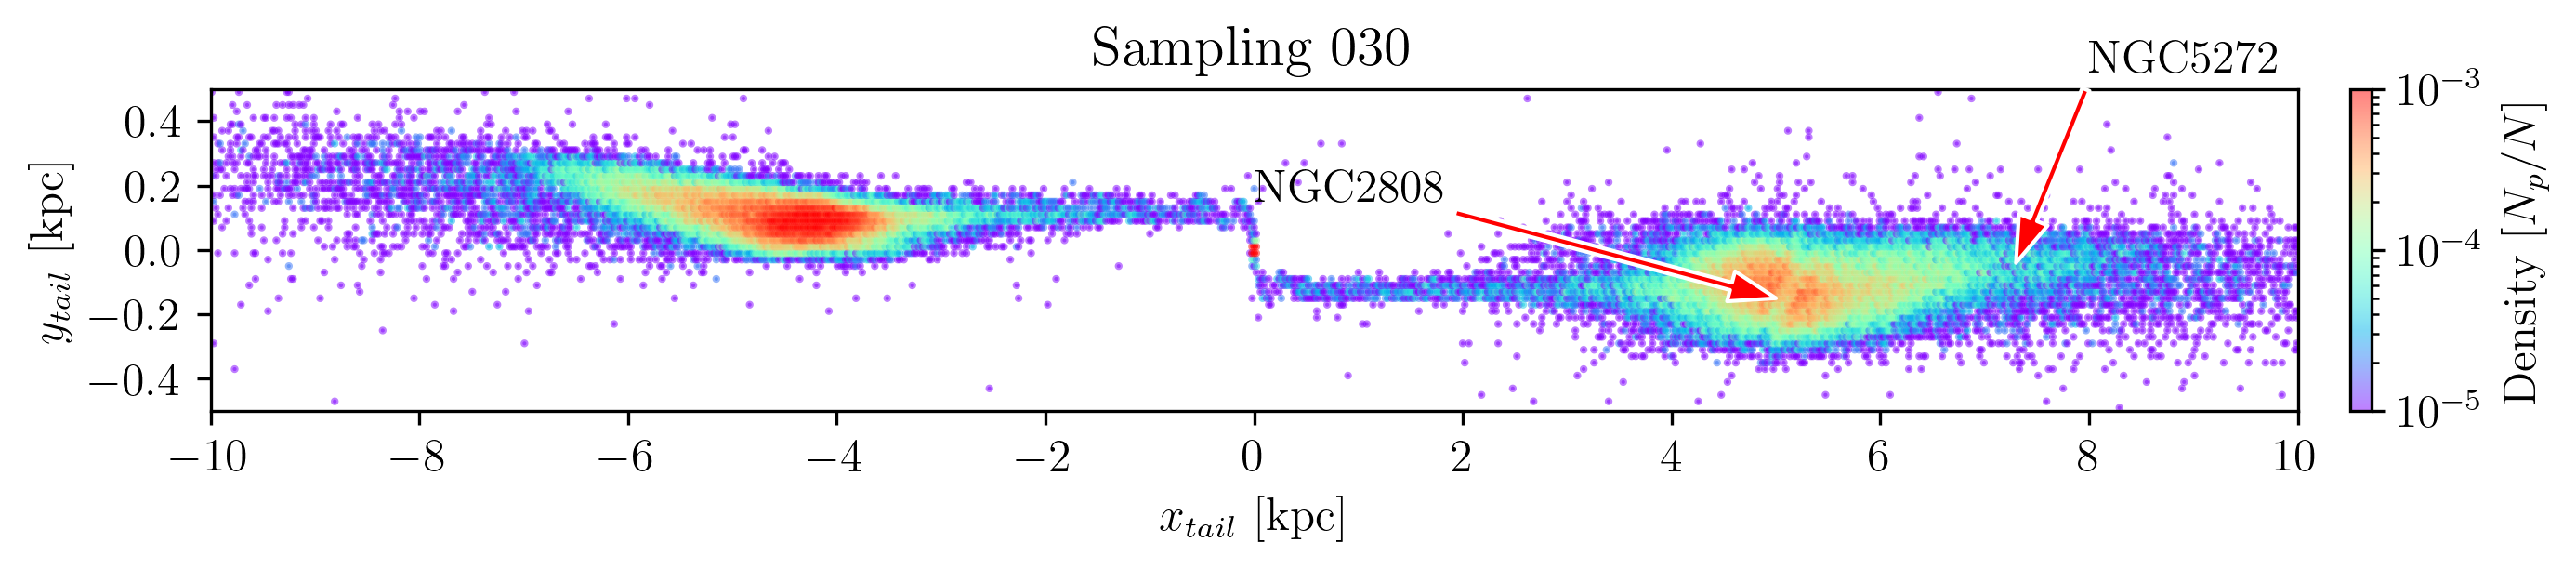
\includegraphics[width=\linewidth]{gallery_of_gaps_monte-carlo-030.png}
      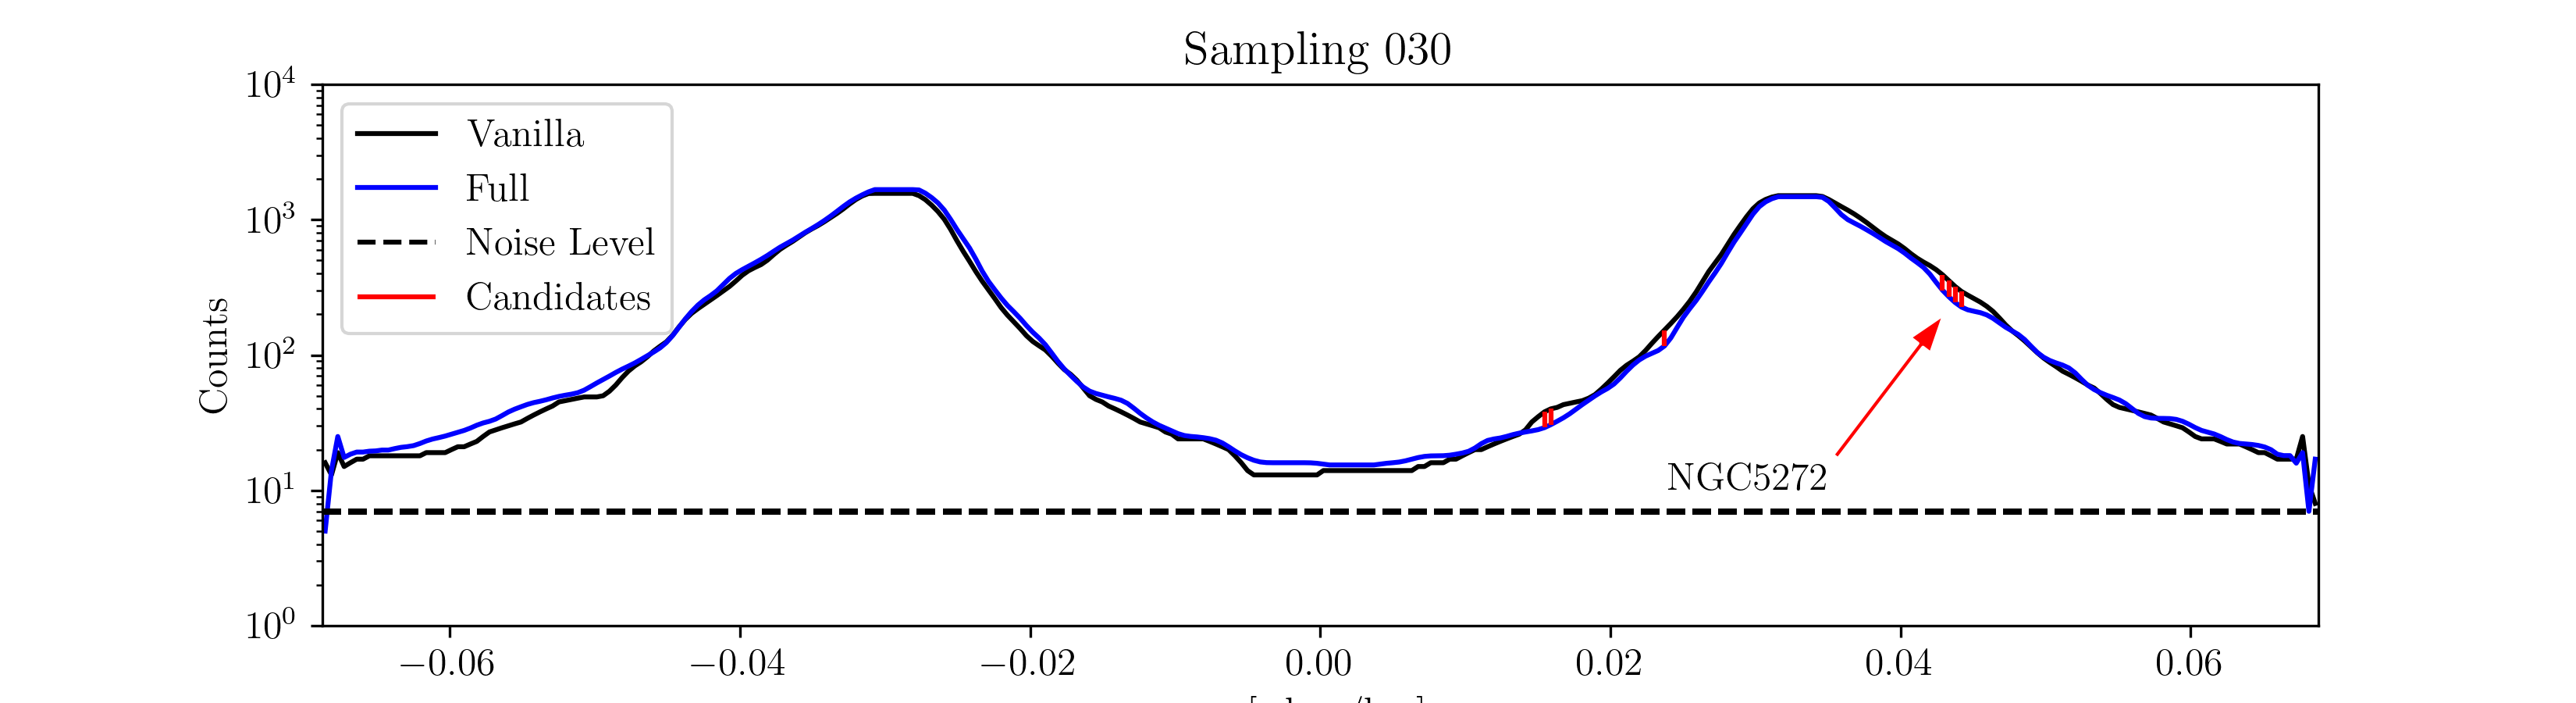
\includegraphics[width=\linewidth]{tau-profile-monte-carlo-030.png}
      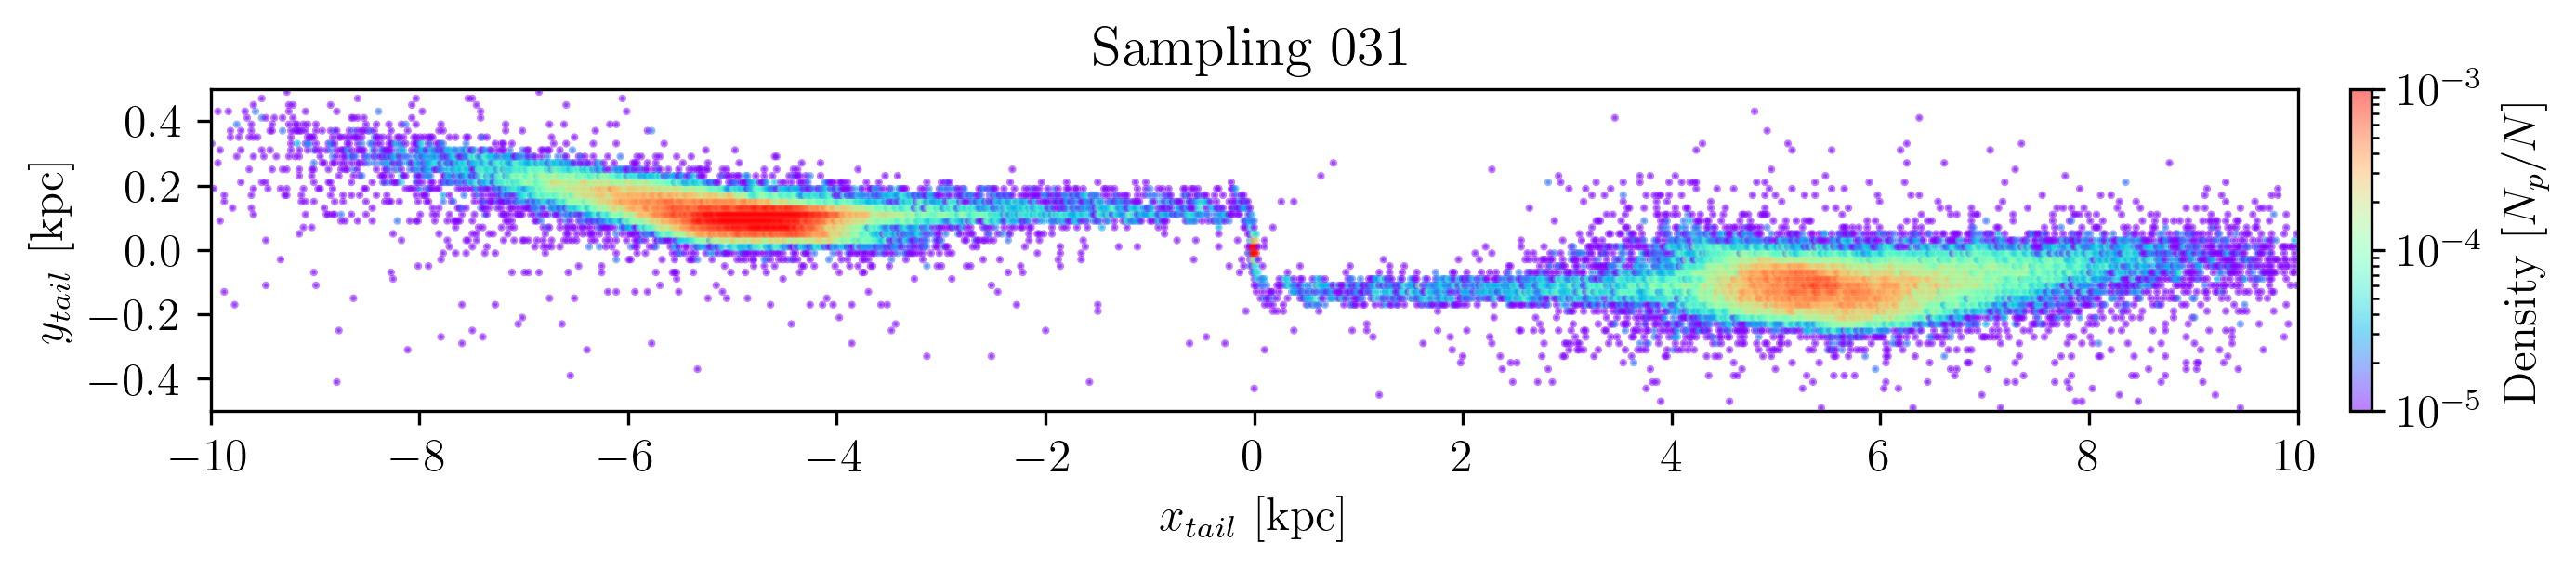
\includegraphics[width=\linewidth]{gallery_of_gaps_monte-carlo-031.png}
      \caption{Gap Gallery}
      \label{fig:TailCoordinates}
    \end{figure*}        


    \begin{figure*}
      \centering
      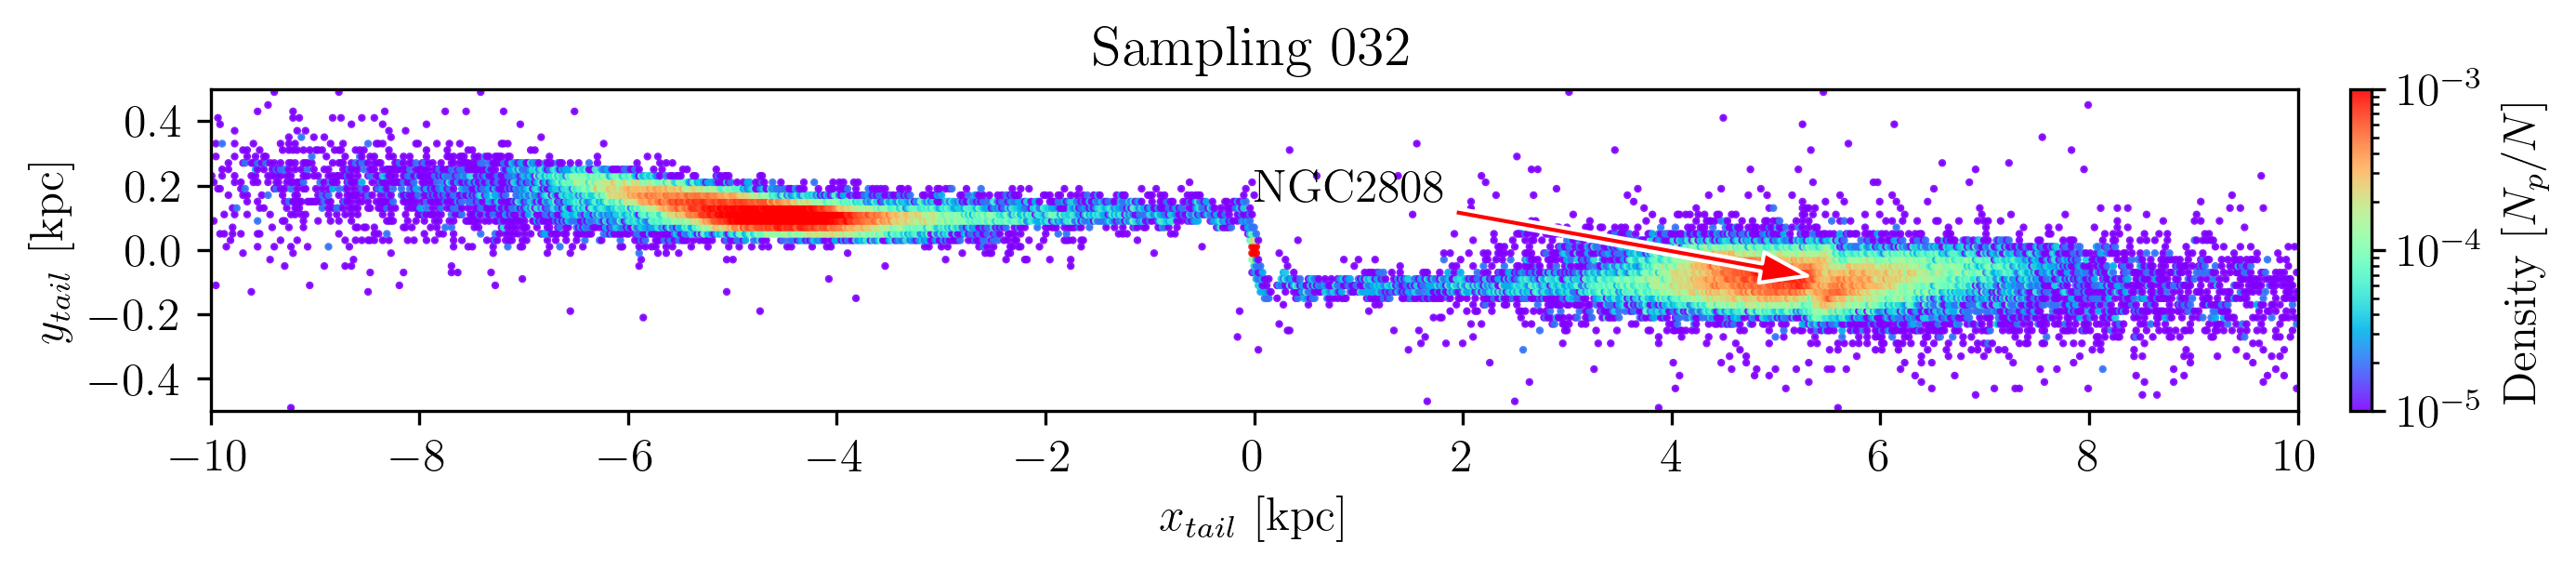
\includegraphics[width=\linewidth]{gallery_of_gaps_monte-carlo-032.png}
      \includegraphics[width=\linewidth]{gallery_of_gaps_monte-carlo-033.png}
      \includegraphics[width=\linewidth]{gallery_of_gaps_monte-carlo-034.png}      
      \includegraphics[width=\linewidth]{gallery_of_gaps_monte-carlo-035.png}
      \includegraphics[width=\linewidth]{gallery_of_gaps_monte-carlo-036.png}      
      \caption{Gap Gallery}
      \label{fig:TailCoordinates}
    \end{figure*}    



    \begin{figure*}
      \centering
      \includegraphics[width=\linewidth]{gallery_of_gaps_monte-carlo-037.png}
      \includegraphics[width=\linewidth]{gallery_of_gaps_monte-carlo-038.png}
      \includegraphics[width=\linewidth]{gallery_of_gaps_monte-carlo-039.png}
      \includegraphics[width=\linewidth]{gallery_of_gaps_monte-carlo-040.png}
      \includegraphics[width=\linewidth]{gallery_of_gaps_monte-carlo-041.png}      
      \caption{Gap Gallery}
      \label{fig:TailCoordinates}
    \end{figure*}        
    \begin{figure*}
      \centering

      \includegraphics[width=\linewidth]{gallery_of_gaps_monte-carlo-042.png}
      \includegraphics[width=\linewidth]{gallery_of_gaps_monte-carlo-043.png}
      \includegraphics[width=\linewidth]{gallery_of_gaps_monte-carlo-044.png}
      \includegraphics[width=\linewidth]{tau-profile-monte-carlo-044.png}
      \caption{Gap Gallery}
      \label{fig:TailCoordinates}
    \end{figure*}   

    \begin{figure*}
      \centering
      \includegraphics[width=\linewidth]{gallery_of_gaps_monte-carlo-046.png}
      \includegraphics[width=\linewidth]{gallery_of_gaps_monte-carlo-047.png}
      \includegraphics[width=\linewidth]{gallery_of_gaps_monte-carlo-048.png}
      \includegraphics[width=\linewidth]{tau-profile-monte-carlo-048.png}
      \includegraphics[width=\linewidth]{gallery_of_gaps_monte-carlo-049.png}
      \caption{Gap Gallery}
      \label{fig:TailCoordinates}
    \end{figure*} 

\end{appendix}



\end{document}